\documentclass[a4paper, 11pt]{article}
\usepackage[utf8]{inputenc}
\usepackage{amsmath, amssymb, amsthm}
\newtheorem{obs}{Observation}
\newtheorem{cor}{Corollary}
\newtheorem{mydef}{Definition}
\usepackage{graphicx}
\usepackage{enumerate}
\usepackage{enumitem}
\usepackage{xcolor}
\usepackage{natbib}
\usepackage{booktabs}
\usepackage{multirow}
\usepackage{caption}
\usepackage{subcaption}
\usepackage{float}
%
\usepackage{hyperref}
\hypersetup{
    colorlinks=true,
    allcolors=blue
}
%
\usepackage[percent]{overpic}

% mauricio: these are used for the benchmark table formatting
\usepackage{array}
\newcolumntype{?}{!{\vrule width 1pt}}
\newcommand{\ra}[1]{\renewcommand{\arraystretch}{#1}}



\bibliographystyle{agsm.bst}

\usepackage{url} % not crucial - just used below for the URL 

%\pdfminorversion=4
% NOTE: To produce blinded version, replace "0" with "1" below.
\newcommand{\blind}{1}

% DON'T change margins - should be 1 inch all around.
% \addtolength{\oddsidemargin}{-.5in}%
% \addtolength{\evensidemargin}{-.5in}%
% \addtolength{\textwidth}{1in}%
% \addtolength{\textheight}{-.3in}%
% \addtolength{\topmargin}{-.8in}%
\usepackage[margin=1in]{geometry}

% ----- used after frontpage stuff to change spacing ------
\def\spacingset#1{\renewcommand{\baselinestretch}%
{#1}\small\normalsize} \spacingset{1.0} % default 1.5 for template
% --------------------------------------------------------

\newcommand{\mau}[1]{{\color{blue}{[Mauricio: #1]}}}
% \DeclareMathOperator*{\minimize}{minimize}
\begin{document}

% ------------ FRONTPAGE STUFF ------------------

\if1\blind % remove \vspace{-2cm} for deliverable
{
  \title{\vspace{-2cm} \bf Large-Scale spatio-temporal Density Smoothing with the Graph-fused Elastic Net: Application to Ride-sourcing Driver Productivity Analysis}
  \author{\textbf{Mauricio Tec}\\
    Department of Statistics and Data Science\\ University of Texas at Austin \vspace{.1cm} \\ 
    \textbf{Natalia Zuniga-Garcia} \\
    Department of Civil, Architectural and Environmental Engineering \\
    University of Texas at Austin \\
    \textbf{James G. Scott}\\
    Department of Information, Risk, and Operations Management \\ Department of Statistics and Data Science\\ University of Texas at Austin \vspace{.1cm}}
  \maketitle
} \fi

\if0\blind
{
  \bigskip
  \bigskip
  \bigskip
  \begin{center}
    {\LARGE\bf Large-Scale spatio-temporal Density Smoothing with the Graph-fused Elastic Net: Application to Ride-sourcing Driver Productivity Analysis}
\end{center}
  \medskip
} \fi

\vspace{-20px}
\begin{abstract}
Ride-sourcing or transportation network companies (TNCs) provide on-demand transportation service for compensation, connecting drivers of personal vehicles with passengers through the use of smartphone applications. This article considers the problem of estimating the probability distribution of the productivity of a driver as a function of space and time. We study data consisting of more than 1 million ride-sourcing trips in Austin, Texas, which are scattered throughout a large graph of 223k vertices, where each vertex represents a traffic analysis zone (TAZ) at a specific hour of the week. We extend existing methods for spatial density smoothing on very large general graphs to the spatio-temporal setting. Our proposed model is designed to overcome two major challenges in dealing with spatio-temporal effects. First, allowing for distinct spatial and temporal dynamics, including different degrees of smoothness. Second, handling missing observations at various vertices of the graph, which arise from fine discretization over the time dimension. Core to our method is an extension of the Graph-Fused Lasso that we refer to as the Graph-fused Elastic Net (GFEN).
\end{abstract}

\noindent%
{\it Keywords:}  spatio-temporal modeling, Graph-fused Lasso, Markov Random Fields, ADMM algorithm, density smoothing, non-parametric density estimation, big data, transportation network companies, ride-sourcing
\vfill

% -------------------------------
\newpage
% \spacingset{1.5} % DON'T change the spacing! % UNCOMMENT BEFORE SUBMISSION


\section{spatio-temporal variation in TNC driver earnings}

\label{sec:intro}

\subsection{Introduction} 

Ride-sourcing or transportation network companies (TNCs), such as Uber and Lyft, provide on-demand transportation service for compensation \citep{shaheen-2016}. TNCs operate as a two-sided market that connects drivers with passengers through the use of mobile applications. 
In recent years, TNCs have experienced rapid growth; for example, Uber saw 5.22 billion trips worldwide in 2018, up from 140 million trips in 2014.  
This growth has posed several challenges to transportation planners, policymakers, and researchers---for example, lack of infrastructure (e.g. at airports), geographical variation in operating rules and regulations, and potential changes in travelers' behavior \citep{smithuber}.  TNCs have also been the subject of controversy because of their aggressive business tactics and sometimes complex pricing systems \citep{li-2019}, whose effects on both rider and driver behavior are not well understood.  

In this paper, we address a fundamental statistical question relevant to all these stakeholders: how best to quantify spatial and temporal variation in TNC driver earnings.  Due to a variety of statistical challenges, which we articulate below, this variation is not well understood---nor are there good methods for estimating this variation reliably, at the scale and speed needed for analyzing millions or billions of trips at high spatial and temporal resolution.  Our goal in this paper is to address this gap.  Specifically, we present a nonparametric method for estimating the probability density $f_{s,t}$, at location $s$ and time $t$, for the productivity of a TNC driver (defined roughly as profit per hour and explained in detail below).   
%and in which RideAustin was responsible for one-third of Austin's ride-sourcing market share, suggesting high representativeness of the data. 
Our method extend the spatial density smoothing framework of \citet{tansey-etal-2017} to the spatio-temporal setting. We discuss the main challenges involved in this extension, and we provide a tool for spatio-temporal density smoothing based on the Graph-fused Elastic Net (GFEN), which can effectively address these challenges.  We accompany this paper with code written in the Julia programming language\footnote{\url{https://github.com/mauriciogtec/GraphFusedElasticNet.jl}}.


We then apply our method using data on more than 1.4 million ride-sourcing trips taken on RideAustin, a local non-profit TNC in Austin, Texas, during a period in 2016-17 when leading national TNCs were temporarily out of the city.\footnote{Uber and Lyft left the city from May 2016 to May 2017 after the Austin City Council passed an ordinance requiring ride-hailing companies to perform fingerprint background checks on drivers, a stipulation that already applies to Austin taxi companies \citep{samuels-2017}.}  Our analysis results in a number of interesting findings---many made possible by the fact that our method yields a full probability distribution of driver earnings, giving us access to such distributional features as quantiles and tail areas.  To give two examples:
\begin{itemize}[itemsep=0pt, partopsep=0pt]
    \item The probability that a TNC driver can expect to earn a living wage in Austin \citep[which we get from][]{nadeau-2017} exhibits high variability with respect to space and time. For a parent of two children who works a typical Saturday late night near downtown Austin, the probability of earning a living wage for the Austin area can exceed 90\%.  But at midday on a Monday far from the city center, this probability can fall below 40\%.
    \item The bottom 10\% of earners among drivers accepting rides at the airport have a productivity below $\$10$/hour in a typical Monday midday.  This is considerably lower than the living wage in Austin for a single adult with no children.
\end{itemize}



\subsection{Ride-Sourcing Productivity Analysis: Background \& Challenges}
\label{subsection:challenges}

Spatio-temporal variation in driver earnings is at the heart of many challenges faced both by the designers of TNC pricing models and by the drivers themselves.  For both the TNC and the drivers, a desirable property of a ride-sourcing platform is what \cite{zuniga-etal-2019} call \emph{destination invariance}, which they define as ``the principle that two drivers dispatched on different trips from the same location at the same time do not envy each other’s expected future income.''  In reality, however, some trip opportunities yield higher continuation payoffs than others, which implies that at least some trips are mis-priced.  From the driver's perspective, this mis-pricing can result in needlessly high volatility in driver earnings, and therefore substantial variation in the likelihood that a driver will earn a living wage.  

Moreover, for both the driver and the TNC, such variation can also result in substantial market efficiencies, potentially impacting service reliability at the level of the whole network \citep{ma-2018}.  For example, drivers may ``chase the surge,'' avoid short trips, or refuse trips from particular pickup locations or within particular time frames, thus leaving riders in some areas without access to the service.\footnote{These examples explain why platforms do not show the trip destination before the driver accepts the ride (e.g., \cite{ignorance, short}).}  Moreover, strategic and/or experienced drivers can learn how to improve their earnings by predicting profitable times and locations, which exacerbates disparities in driver earnings and satisfaction, as found by \citet{gender}. 
TNCs respond to this reality in a variety of ways.  For example, Uber and Lyft tried to provide drivers with more flexibility by adding destination filters, where drivers can select the desired drop-off location that would allow them to relocate themselves as they preferred \citep{filter1, lyft}. However, this feature caused a negative impact on the platform by increasing riders' waiting time and other drivers' pick-up time, as strategic drivers used the filter to select trips with better earning potential, leading Uber to cap drivers' usage of this feature at twice per day \citep{filter2}. 

Recent research efforts have addressed ride-sourcing's spatial mis-pricing problem by proposing different pricing strategies and driver-passenger matching functions. Some examples that have been studied include incorporating spatial surge pricing models \citep{spatial3, spatial2}, search and matching models \citep{friction8, spatial4, spatial5, spatial15}, non-linear pricing models \citep{friction9}, and spatio-temporal pricing mechanisms \citep{ma-2018}. 

%In the transportation research literature, productivity has been measured by accounting for idle and reach time \citep{idle}, average speed \citep{can}, capacity utilization rate \citep{can, capacity}, average earning per unit time \citep{learning}, and fuel cost \citep{fuel}.

In this paper, we do not explicitly consider the question of how to design a better TNC pricing model.  Rather, we take the perspective that before one can design such pricing models that mitigate spatio-temporal variation in driver earnings, one must first quantify the extent of that variation---and we therefore seek to provide a scalable, reliable method for doing so.  But this poses a complex set of statistical challenges.  First, the availability of public ride-sourcing data is limited, leading some authors to rely on simulations \citep{ma-2018, spatial2} or to limit their research to taxi-only data \citep{spatial3, spatial4}.  Second, when available, spatio-temporal information is subject to noise and high sparsity, where many combinations of space and time have no or very little data.  This has previously led researchers to aggregate the data into large spatial and/or temporal (e.g. peak vs. off-peak) blocks, as in \citet{spatial3}, \citet{spatial4}, and \citet{friction8}).  This helps with data sparsity, but compromises the ability to find valuable high-resolution insights.  Low spatio-temporal resolution owing to data sparsity can be especially problematic when analyzing detailed pricing scheme consequences.  We address this problem by relying on modern spatial smoothing/interpolation techniques that penalize total variation---although as we describe below, we must modify these techniques to handle the data-sparsity problem in a way that still yields sensible interpolations.


% \subsection{RideAustin Dataset: Challenges for Spatio-temporal Modeling}


Our approach encodes spatio-temporal structure using a graph, where each vertex corresponds to a traffic analysis zone (TAZ)\footnote{TAZs are geographic areas dividing a planning region into relatively similar areas of land use and land activity.} at a specific hour of the week, and where edges are used to denote geographical and temporal adjacency. Austin TAZs are shown in Figure \ref{fig:areatypes}. This results in a graph of 223k vertices, one for each location at a specific time; our goal is to estimate a full probability distribution for the productivity of a driver at each one of these vertices (we provide further details about the construction of the graph in section \ref{section:graph}.)  Owing to the size of the graph, we shall build upon the scalable spatial density smoothing framework of \citet{tansey-etal-2017}, extending it to the spatio-temporal setting. \citet{zuniga-etal-2019} applied this technique to the RideAustin dataset and showed it to be effective in modeling purely spatial effects. However, there are two main challenges that are unique to the spatio-temporal setting and that we must addressed in order to accomplish our goal.

\begin{figure}[tb]
    % \begin{minipage}[tb]{.5\linewidth}
    %     \centering
    %     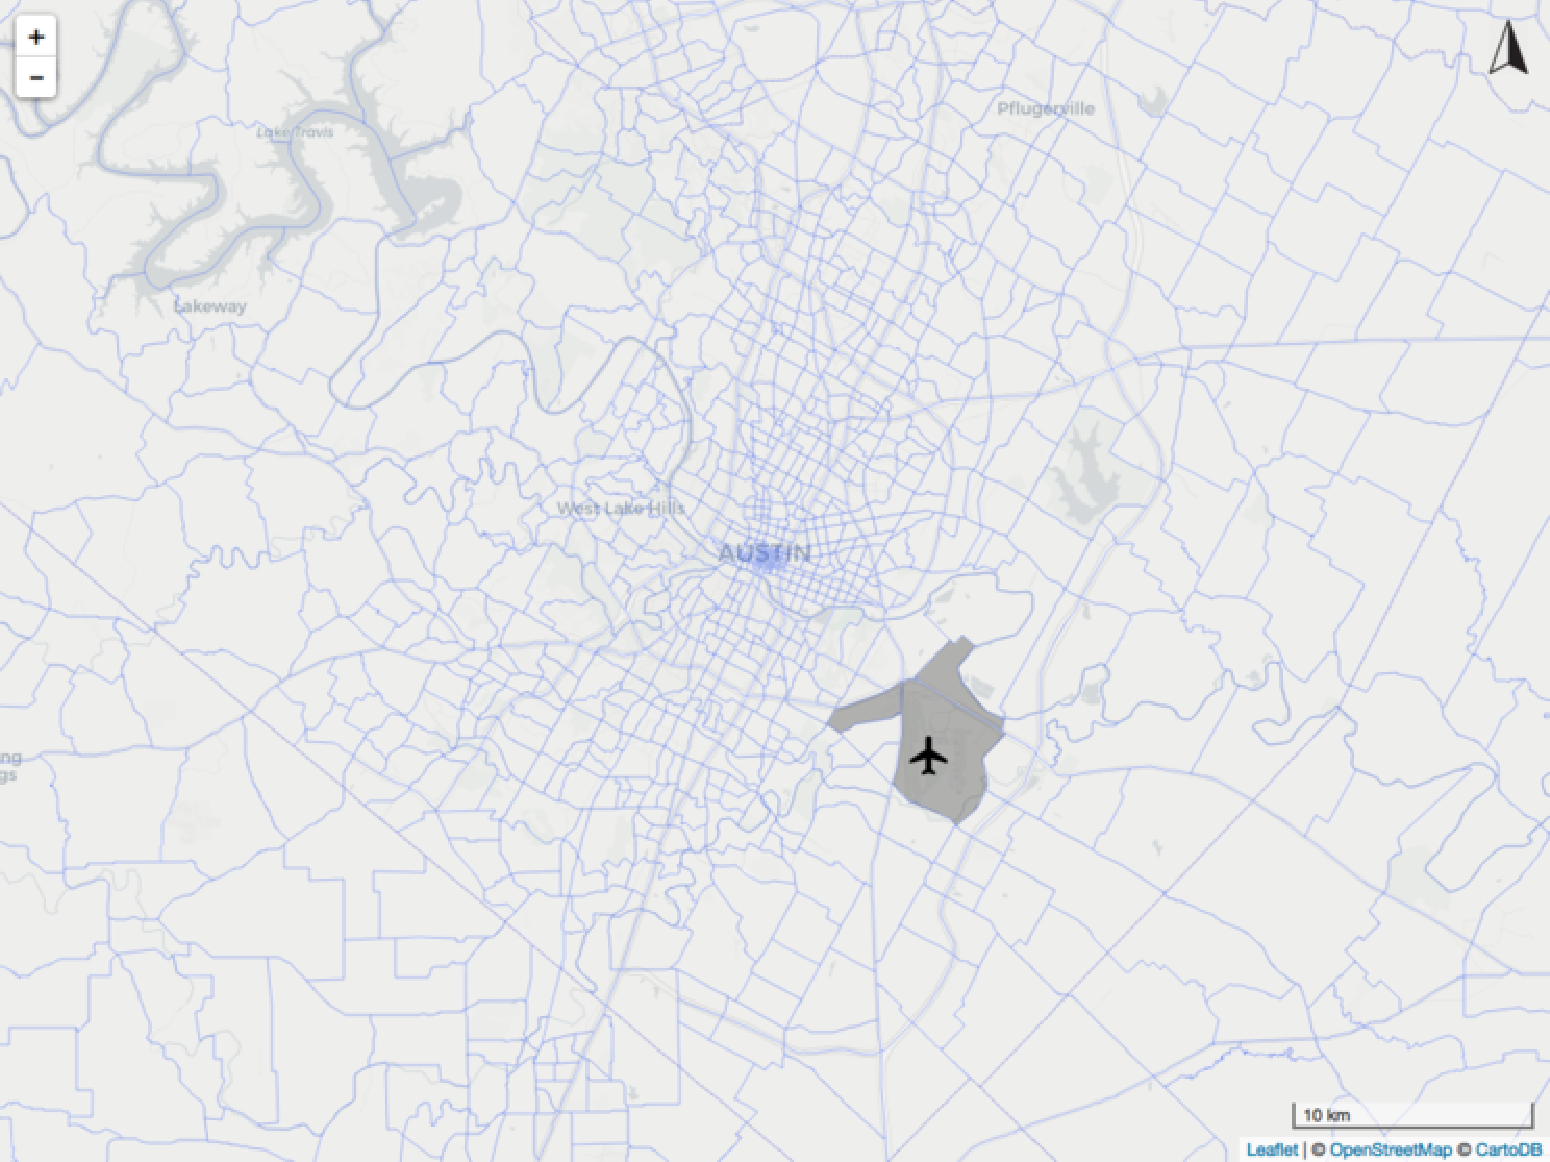
\includegraphics[width=0.99\linewidth]{img/tazs.pdf}
    %     \subcaption{TAZs in Austin (airport shaded)}
    %     \label{fig:areatypes:a}
    % \end{minipage}%
            \centering
    \begin{minipage}[tb]{.8\linewidth}

		\begin{overpic}[width=0.99\linewidth]{img/areatypes.pdf}
			\put(0,0){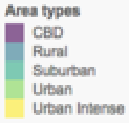
\includegraphics[width=1.5cm]{img/areatypes_legend.pdf}}
		\end{overpic}
		\subcaption{Area types}
		\label{fig:areatypes:b}
    \end{minipage}
    \caption{Austin traffic analysis zones (TAZs) classified by area type. Blue lines indicate TAZ boundaries.  The central business district (CBD), which contain the downtown, is shown in purple.} \label{fig:areatypes}
\end{figure}


The first challenge comes from the question of how to smooth the raw data while still capturing important spatio-temporal effects. The space and time dimensions have different units and physical interpretations, suggesting that spatial versus temporal edges must be  treated differently. Moreover, effects in space and time are likely to be a mix of smooth and non-smooth transitions. For example, the productivity of a driver may change drastically from one side to another of a highway or a river, but it would most likely be similar or even constant across highly interconnected regions with no obvious barriers.  In the time dimension, by contrast, effects are more likely to be smooth, and yet there may still be sudden transitions caused by specific events, such as increased temporal density of airport arrivals.  The challenge here is to allow for separate but parsimonious spatial and temporal dynamics that incorporate a mix of both smooth and non-smooth features.

The second challenge arises from the fact that many vertices in our graph will have no data.  For the RideAustin dataset, where we discretize by the hour of the week, 45.8\% of the vertices of the graph have no observations.  (Every TAZ in our data set had at least one observation at some point of the week, but many do not have observations for every hour of the week.)  The challenge here is to develop a method that can borrow information efficiently across spatial and temporal adjacenties, estimating a density at every location for every hour, even if no data was observed.

\subsection{Proposed Methodology}

To estimate full densities in a spatio-temporal graph we will extend the methodology of \citet{tansey-etal-2017}, which uses a non-parametric density estimation technique coupled with the graph-fused lasso to provide a highly scalable and parallelizable spatial density estimation technique. Their technique consists of three steps:
\begin{enumerate}
    \item Split the overall problem into sub-problems recursively partitioning the variable's support into a series of half-spaces, each described by a conditional probability. 
    \item Smooth each half-space probability across space in such a way that encourages similarity between adjacent nodes of a graph.
    \item Merge the smoothed half-space probabilities to yield full density estimates at each node.
\end{enumerate}

In this paper we extend the analysis of \citet{zuniga-etal-2019} who applied a methodology based on the Graph-fused Lasso (GFL) to effectively estimate spatial effects on driver productivity. Our measure of productivity is the same as the one used in their paper. However, there are three main differences between their approach and one taken here. First, \citet{zuniga-etal-2019} only estimate spatial effects; and they only treat time by splitting the dataset into on-peak, off-peak, week, and weekend periods. Instead, we consider spatio-temporal effects with fine time granularity. Second, the authors only estimate mean effects, whereas here we seek full densities. In particular, we exploit spatio-temporal quantiles and measures of spread learned from our estimated distributions to enrich our analysis. Finally, they only model the type of locally constant effects that are well captured by the GFL (see \citet{tibshirani-2015}), whereas here we will consider both smooth and non-smooth effects.

In this paper, steps 1 and 3 will be identical, however, the methodology for step 2 based on the GFL is directly applicable to the spatio-temporal setting since it cannot directly address the challenges mentioned in the previous section. The first challenge will not be met because, as mentioned before, the GFL objective only considers non-smooth or locally-constant effects. The second challenge will also fail to be met because, as we shall explain in section \ref{section:methodology}, the GFL objective will no longer be strictly convex if there are vertices without observations. As a consequence, it does not perform any interpolation from neighbouring regions in the absence of data. Ignoring this fact, or resolving it in a naive way, can lead to unexpected and undesirable behavior. 

To address these limitations, we propose to combine the traditional L1 total variation penalty used by the GFL with an additional L2 total variation term. This will have the effect of enabling both smooth and non-smooth transitions. The L2 penalty is essentially equivalent to using a Gaussian Markov Random Field \citep{cressie-1993}. We call the resulting method the Graph-fused Elastic Net (GFEN), as an analogy to the elastic net regularization method for regression \citep{zou-2005}. Adding the extra L2 regularization can be regarded as adding an empirical prior added to the GFL objective that shrinks a value towards the average estimate of its neighboring vertices; having the effect of interpolating data in the absence of observations.  Figure \ref{fig:densities-sample} shows an example of the estimated densities for three locations: airport, downtown\footnote{We identify downtown with the TAZ that contains the intersection of Guadalupe \& 6th, which has very high trip demand.} and Red River \& 12th\footnote{Red River \& 12th street is a small TAZ next to downtown but with low trip count}; and for two selected times: Sunday 3am and Monday 1pm, which are characterized respectively by high and low demand. Figure \ref{fig:densities-sample} shows that the high demand of Sunday 3am increases productivity more in the downtown area than in the airport. Second, the image also shows that even with no data observed at Red River \& 12th---which is geographically next to downtown---it is still possible to learn a sensible density model.

\begin{figure}[tb]
    \centering
    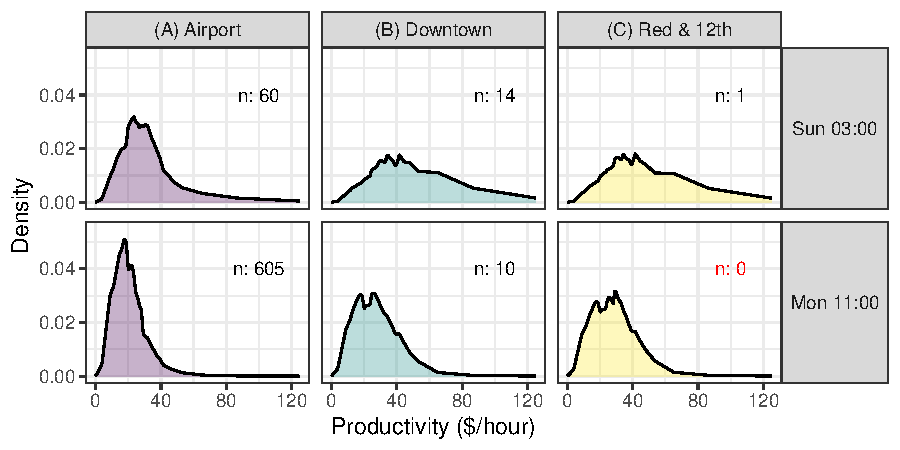
\includegraphics[width=12cm, height=6cm]{img/densities_spacetime_sample.pdf}
    \caption{Shows examples of our density estimation methodology with the GFEN for some selected locations and hours. The number of data points at each specific location and time is indicated with $n$ next to each density. Red River \& 12th is a small TAZ with few observations next to downtown. The model borrows information from neighboring regions to estimate a model in this vertex.}
    \label{fig:densities-sample}
\end{figure}

We will provide an algorithm for implementing the GFEN using a modified version of the highly-parallelizable ADMM algorithm presented by \citet{tansey-scott-2015}. The resulting algorithm will still consist of linear time updates and will scale to massive graphs just as its purely GFL-based counterpart.

The fact that the GFEN is able to handle smooth and non-smooth transitions, as well as dealing with differentiated spatial and temporal dynamics, comes at the expense of increasing the number of hyperparameters to tune. First, solution path approaches that are typically used to tune the GFL penalty hyperparameter will no longer work, as they are based on one dimension and one variable to tune (see \citet{tibshirani-2015}). Second, tuning methods based on information criteria that depend on degrees of freedom (e.g. BIC) are harder to compute, since the smoothness induced by the added L2 total variaton penalty makes the estimation of the effective degrees of freedom very hard. To alleviate the situation, we propose a framework based on Bayesian optimization \citep{shahriari-etal-2016} and cross-validation to select the best hyperparameters. This approach was successful when applied to our RideAustin dataset.
% 

\subsection{Statistical Background \& Related Work}


Our methods build on two independent lines of work: first, spatial density smoothing over a graph; second, extensions of spatial models to spatio-temporal models. We do not attempt to provide a fully detailed literature review of these mature fields. But we will outline the relevant work most closely related to our methodological approach.

First, for background on spatial density smoothing over graphs, we refer the reader to the paper by \citet{tansey-etal-2017}, as well as the references therein. Our method is an extension of their methodology (see the previous section) that uses the same technique of representing a probability distribution via a recursive dyadic partition. This technique has been widely used---for example, in multiscale models for Poisson and multinomial estimation \citep{fryzlewicz-nason-2002, jansen-2006, willett-nowak-2007}, and in nonparametric Bayesian inference via Polya-tree priors \citep{mauldin-1992, lavine-1992, lavine-1994}. Another paper that we refer the reader to for a review is due to \citet{zhao-hanson-2011}, who take a related approach by coupling a Polya-tree prior with a conditional autoregressive (CAR) prior in a fully Bayesian model. The scalable algorithm for spatial denoising over a general graph that we take as departure point for this paper is provided by \citet{tansey-scott-2015}, which in turn builds on computationally efficient estimation for the class of convex optimization problem that arises from the GFL model, including the papers by \citet{tibshirani-taylor-2011, ramdas-tibshirani-2016, wang-2016}. 

The GFL is related to the technique known as total variation denoising in the signal processing literature \citep{getreuer-2012}. The total variation penalty based on the L1-norm is used to denoise images by encouraging locally constant effects with sharp edge boundaries. There are highly scalable algorithms to implement such models for image data, for example, based on the parametric max-flow algorithm \citep{hochbaum-2001, chambolle-darbon-2009}. Modeling spatial effects using total variation denoising with the L2-norm is a special case of a Gaussian Markov Random Fields (GMRF) \citep{rue-held-2005}. GMRFs are also common in the image denoising literature. A recent linear-time algorithm is provided by \citet{yasuda-2018}. GMRFs are well-known to promote smooth edges as opposed to the sharp contrasts encouraged by the L1-norm. Note that these image denoising techniques do not address the problem of full density estimation, since they are primarily concerned with denoising a signal. Moreover, they are typically designed for rectangular grids, which are common with image and other signal data.

In the statistics literature, the GFL is also related to some work in Bayesian inference for spatial data models. Specifically, it is similar to conditional auto-regressive (CAR) models \citep{besag-1974}, which also effect spatial smoothing by discouraging large pairwise differences across edges in a graph. Bayesian models consider the approach of estimating the density from the point of view of the posterior predictive density. Non-parametric Bayesian approaches for density estimation with spatial smoothing were investigated by \citet{gelfand-2015}, \citet{reich-fuentes-2007}, \citet{rodriguez-2010}, among many others.  Also highly related is the approach by \citet{li-2015}, who propose a non-parametric Bayesian models for areal data that can detect boundaries between spatial neighbors where a sharp change occurs. We refer the interested readers to these papers and their references for more detail.


We now consider the background work regarding the extension of spatial models to spatio-temporal settings. In the statistics literature, the have been two main approaches for this task. The first approach consists of treating time as an additional undifferentiated dimension from space. This approach would typically involve estimating a covariance matrix that includes both the space and time dimensions, e.g. \citep{cressie-huang-1999, allcroft-glasbey-2003}. More generally, this approach can be used for all kernel methods \citep{bashtannyk-hyndman-2001}. The drawback of such approaches is that kernel methods depend on a meaningful distance measure, which is problematic for spatio-temporal modeling since space and time have different units and physical interpretations. 


The second approach within the statistics literature is to use dynamic probabilistic models \citep{stroud-2001}. In this approach, the parameters of a spatial model are assumed to change smoothly over time following an auto-regressive model. For example, in \citep{cressie-2010} and \citep{katzfuss-cressie-2011}, the authors model spatial effects using low-rank basis approximations to the spatial correlation function and auto-regressive processes for the temporal dependence. Closely related appraoches combining low-rank basis approximation and dynamical modelsin the fully Bayesian setting can be found in \citep{katzfuss-cressie-2012} and \citep{finley-2012}. Auto-regressive processes based on the Gaussian distribution are essentially GMRFs on the temporal dimension and are related to the Kalman Filter. An example application of GMRFs for both spatial and temporal effects in disease modeling is given by \citet{rushworth-2017}. As pointed out by \citet{xu-2015}, GMRFs have the advantage of being able to deal with missing observations at some point in time, which is common in geostatistical practice and is one of the challenges for the RideAustin dataset.

In the video denoising literature, the smooth transitions induced by the GMRF model inadequately model motion, which has lead to the search for alternative transition distributions for Markov Random Fields---for example, \citet{chen-tang-2007} consider estimating a non-parametric transition distribution for the temporal dimension. Total variation denoising based on the L1-norm have also been used for video denoising tasks. For a recent survey we refer the reader to the introduction of \citep{arias-morel-2018} and \citep{parisotto-2019}. However, similar to the image denoising case, most of these methods are designed to work for rectangular grid only and not for general graphs. They are also generally focused on denoising a signal, and not on density estimation.



\subsection{Outline of the Paper}

In Section \ref{section:methodology} we explain the methodology taken in this paper to solve the key challenges mentioned in Subsection \ref{subsection:challenges}. In Section \ref{section:simulation} we show experiments that illustrate our method with synthetic data and compare the performance of the GFL, GMRF, and GFEN. In Section \ref{section:case-study} we implement our proposed methodology to the RideAustin dataset and use it to extract meaningful insights from the data.

\section{Methodology}
\label{section:methodology}

In this section we briefly describe the notation and methodology for spatio-temporal smoothing.

\subsection{Spatio-temporal graphs}

We represent represent space and time using discrete structures, more precisely, using an undirected graph $G=(V, E)$ where $V$ is a set of vertices or space-time nodes and $E$ is the of edges connecting neighboring nodes in time and space. While the methods explain in this section are designed for general graphs, in this problem we are concerned for graphs that encode a spatio-temporal structure. Therefore, we assume that $G$ has the following structure:
\begin{itemize}[partopsep=0pt, itemsep=0pt]
    \item There is exactly one node for every location and in each moment in time. The vertex set can be written as $V = S \times T$ where $S$ and $T$ are the sets of locations and times respectively. The temporal slice at location $s$ is the set $\{s\} \times T$ and the spatial slice at time $t$ is the set $S \times \{t\}$.
    \item Edges are either spatial or temporal. Thus the set of edges can be written as a disjoint union $E = E_S \cup E_T$ where $E_S$ connects nodes in the same spatial slice and $E_T$ connects nodes in the same temporal slice.
\end{itemize}
 At each vertex $(s,t)$ we have a collection of observed data $$\textbf{y}^{(s,t)}=\left\{y^{(s,t)}_1,\hdots,y^{(s,t)}_{N^{(s,t)}}\right\},
 \quad y^{(s,t)}_i \overset{iid}{\sim} f(s,t)$$
 where $f(s,t)$ is the density distribution that we seek to estimate. The goal of spatio-temporal graph-based density smoothing is to estimate density $f(s,t)$ in a way that borrows information from neighboring regions. Graph smoothing is particularly useful when $N^{(s,t)}$ is small or zero in some vertices. 

\subsection{Density estimation with a binary partition}
\label{sec:binary-patition}


 We now briefly review the technique of estimating a density based on a recursive dyadic partition as proposed by \citet{tansey-etal-2017}. The assumptions for this approach are:
\begin{enumerate}[partopsep=0pt, itemsep=0pt]
    \item The output space of the data is a known set $B$, so that $\mathbf{y}^{(s,t)}\subset B$ for all $(s,t)\in V$;
    \item We can recursively define a dyadic partitioning scheme as follows. First, we assume that $B$ can be written as a union of disjoint subsets $B= B_0 \cup B_1$. Now, given the set $B_\gamma$ with $\gamma\in\{0,1\}^k$, then $B_\gamma$ can be written as a disjoint union of subsets $B_\gamma = B_{\gamma0} \cup B_{\gamma1}$. We refer to $B_{\gamma0}$ and $B_{\gamma1}$ as the left children and right children respectively of the parent $B_\gamma$.
\end{enumerate}
The partitioning scheme defines a depth-$K$ binary tree structure on $B$ given by
$$
B^{(K)} := \bigcup_{k=1}^K \left\{B_\gamma \mid \gamma \in \left\{0,1\right\}^k\right\}.
$$
The nodes $B_\gamma$ where $\gamma \in \{0,1\}^K$ is of length $K$ are called the terminal nodes or leaves of the tree. Note that for every $k \leq K$, we have a decomposition of $B$ into $2^k$ disjoint sets
$$
B = \bigcup_{\gamma\in\{0,1\}^k} B_\gamma.
$$

 To illustrate the idea, suppose $B=[0,1)$. We could then define $B_0 = [0,1/2)$ and $B_1=[1/2,1)$. Similarly, we could write $B_{00}=[0,1/4)$, $B_{01}=[1/4,1/2)$, $B_{10}=[1/2,3/4)$ and $B_{11}=[3/4,1)$ and so on. Later in this section, we will discuss some the implications of different splitting schemes. 

Assume now we are given a partition tree $B^{(K)}$ and let $Y \sim f$ be some random variable with output space $B$. Then \citet{tansey-etal-2017} propose to estimate the quantities
$$
\omega_\gamma = P(Y \in B_{\gamma0} \mid Y \in B_\gamma)
$$
which is the probability of a data point belonging to the left child $B_{\gamma0}$ provided it belongs to the parent $B_\gamma$. We can use the variables $\omega_\gamma$ to give a non-parametric estimate of the probability distribution of $Y$ on the leaves of tree. The resolution level is determined by the depth of the tree $K$. More precisely, for any $\gamma=(\gamma_1,\hdots,\gamma_K)\in\{0,1\}^K$ we have
\begin{equation}\label{eq:recover-probability}
\begin{aligned}
P(Y \in B_\gamma) &= \prod_{j=0}^{K-1} \mathrm{Bernoulli}\left(\gamma_{j+1} \mid \omega_{(\gamma_1,\hdots,\gamma_j)}\right).  \\
& = \prod_{j=0}^{K-1} \omega_{(\gamma_1,\hdots,\gamma_j)}^{\gamma_{j+1}}\left(1 - \omega_{(\gamma_1,\hdots,\gamma_j)}\right)^{1 - \gamma_{j+1}}.
\end{aligned}
\end{equation}
We now put the above formulation back into our spatio-temporal model. Define $m^{(s,t)}_\gamma$ as the count of total observations of $\mathbf{y}^{(s,t)}$ that fall within $B_\gamma$. Then for each non-terminal node $B_\gamma$ we have
\begin{equation}\label{eq:binomial-model}
m_{\gamma0}^{(s,t)} \sim \mathrm{Binomial}(\omega^{(s,t)}_\gamma, m_\gamma^{(s,t)})
\end{equation}
The models defined by expression \eqref{eq:binomial-model} enable us to learn a estimate the $\omega_\gamma$ from the data. It will be convenient to reparametrize \eqref{eq:binomial-model} in terms of the log-odds $\beta_\gamma$, so that $\omega_\gamma = \sigma(\beta_\gamma) := (1 + \exp(-\beta_\gamma))^{-1}$. Thus, for each vertex $(s,t)$ and for each non-terminal node $B_\gamma$ the corresponding negative log-likelihood function is
\begin{equation}\label{eq:loglikelihood}
\begin{aligned}
l_\gamma(\mathbf{y}^{(s,t)}, \beta_\gamma^{(s,t)}) & := - m_{\gamma0}^{(s,t)}\log \sigma(\beta^{(s,t)}_\gamma) - m_{\gamma1} \log (1 - \sigma(\beta^{(s,t)}_\gamma)). 
\end{aligned}    
\end{equation}

\subsection{The Graph-Fused Lasso (GFL)}\label{sec:gfl}

In section \ref{sec:binary-patition} we presented a binomial probability model for the splitting probability at each node of a tree structure. Which corresponds to step 1 in the split/smooth/merge approach for density smoothing. In this section we will show how to use graph smoothing for step 2 for spatio-temporal graphs. Since step 2 is identical for every node of the tree $B_\gamma$, we will drop $\gamma$ from the notation in the interest of presentation. 

The idea of graph-based denoising is to penalize big differences along edges. Let $\lambda_{vw} > 0$ be a penalization parameter for each edge $vw \in E$. Then the GFL objective is
\begin{equation}\label{eq:gfl}
\begin{aligned}
\operatornamewithlimits{minimize}_{\beta} \quad \sum_{v \in V} l(\mathbf{y}^{(v)}, \beta^{(v)} ) + \sum_{vw\in E} \lambda_{vw} \left\lvert \beta^{(v)} - \beta^{(w)}\right\rvert.
\end{aligned}    
\end{equation}
where $l$ is the loss function defined in expression \eqref{eq:loglikelihood}. Traditionally, the penalization parameters $\lambda_{vw}$ are considered uniform for all edges. However, when dealing with spatio-temporal graphs, we will assume that the penalization parameter is constant with value $\lambda_S>0$ for spatial edges and also constant but with a potentially different value $\lambda_T>0$ for the time edges. In this case, the GFL objective becomes 

\begin{equation}\label{eq:gfl-spatio-temporal}
\begin{aligned}
\operatornamewithlimits{minimize}_{\beta} \quad \sum_{v \in V} l(\mathbf{y}^{(s,t)}, \beta^{(v)}) + \lambda_S \sum_{vw\in E_S} \left\lvert \beta^{(v)} - \beta^{(w)}\right\rvert + \lambda_T \sum_{vw\in E_T} \left\lvert \beta^{(v)} - \beta^{(w)}\right\rvert.
\end{aligned}    
\end{equation}


The model defined by expression \eqref{eq:gfl-spatio-temporal} will be an excellent model for smoothing when there is a suspicion that the underlying densities have locally constant spatio-temporal effects; meaning that the underlying model parameters $\beta$'s are identical for close regions or \textit{plateaus} and with sharp transitions between adjacent \textit{plateaus}. This assumption can be very restrictive when there is an argument in favor of smooth transitions. For example, when temporal dynamics change softly. Moreover, as we will illustrate in the upcoming sections, expressions \eqref{eq:gfl} and \eqref{eq:gfl-spatio-temporal} may not be strictly convex in the presence of missing observation at some vertices. Concretely, this would be equivalent to some of the terms $l(\beta^{(v)})$ be missing. Our introduction of the Graph-fused Elastic Net is motivated by these two scenarios.
        
\subsection{The GFL Behavior with Missing Data}
\label{subsection:gfl-non-convex}

Consider the following trivial observation.
\begin{obs}\label{obs:non-convex}  Given fixed values $a < b$. Then 
$$|x - a| + |b - x| = b - a$$
for all $a < x < b$. 
\end{obs}
The set-up of observation \ref{obs:non-convex}, while seemingly harmless, is shown to provide an intuition of how the GFL objective does not have a unique solution with missing data. To illustrate this, suppose that the GFL objective \eqref{eq:gfl} is solved for some graph, such that in this graph there is a node with estimate $x$ that has only two neighbors with corresponding estimates $a$ and $b$. Then any value of $x$ in between $a$ and $b$ leads to the same value of the total variation L1 penalty. Thus, if there is no data at the vertex corresponding to $x$, then its value cannot be inferred from the GFL objective alone. The same logic can be extrapolated to more general graphs and missingness patterns. 

A simple solution to remedy the lack of strong convexity with missing data in the GFL object is to add a regularization term. It might be tempting to use a regularizer shrinking towards zero, such as a Ridge or Lasso penalty. However those solutions might have an undesirable effect. To illustrate this, considered the following simplified scenario.
 
 \begin{obs}\label{obs:dont-shrink}
 Given fixed values $a < b$. Then $x^*=a$ is the unique solution to the following optimization problem 
$$
\operatornamewithlimits{minimize}_{x\in\mathbb{R}} \; |x - a| + |b - x| + \rho(x) 
$$
where $\rho(x)$ is any penalization shrinking towards zero. In particular, this holds true for $\rho(x)=\lvert x \rvert$ or $\rho(x)=\lVert x \rVert ^2$.
 \end{obs}
Thus, shrinking penalties added to the GFL objective \eqref{eq:gfl} will have a very strong informative effect. It is worth putting observation \ref{obs:dont-shrink} in the context of density estimation with a partition tree as shown in section \ref{sec:binary-patition}. The effect of shrinking the binomial log-odds coefficients towards zero will favor density estimates that are closer to a uniform distribution in the output space. This would happen since the model would tend to assign equal probabilities to each binary partition. This in practice can result in estimates biased towards heavy-tails. 

We first consider what would happen if we replaced the GFL penalty by the GMRF penalty in observation \ref{obs:non-convex}. Now there is a unique solution which is essentially the average of the neighboring points.

 \begin{obs}
 Given fixed values $a < b$. Then the optimization problem
$$
\operatornamewithlimits{minimize}_{x\in\mathbb{R}} \; (x - a)^2 + (b - x)^2.
$$
has $x^*=(b - a) / 2$ as the unique solution.
\end{obs}
In the absence of data, the GMRF penalty is minimized when each vertex is equal to the average of its neighbors. Contrary to the GFL penalty, as long as one-vertex has data, and the negative loglikelihood is convex, the GMRF penalty will lead to a strictly convex objective. We can finalize our series of observations in simplified scenarios considering what would happen if both the L1 and L2 penalties are combined.
\begin{obs}\label{obs:combined}
 Given fixed values $a < b$. Then the optimization problem 
$$
\operatornamewithlimits{minimize}_{x\in\mathbb{R}} \; \lambda_1 \left[|x - a| + |b - a|\right] + \lambda_2 \left[(x - a)^2 + (b - x)^2\right]
$$
has $x^*=(b - a) / 2$ as the unique solution independently of the values of $\lambda_1 > 0$ and $\lambda_2 > 0$.
\end{obs}
Observation \ref{obs:combined} provides an intuition of the effect of adding the GMRF penalty to the GFL penalty under a missing data scenario. We can argue that the extra GMRF penalty will have the effect of linearly interpolating from neighboring estimates in regions with missing data. 


\subsection{The Graph-fused Elastic Net (GFEN)}

We are ready to define the optimization problem solved by the Graph-fused Elastic Net (GFEN). First, let us introduce a notation for the total variation penalty for the Lp norm.

\begin{mydef}[Lp total variation]
Given a graph $G=(V, E)$ and a set of scalar parameters $\beta=\{\beta^{(v)}\}_{v \in V}$ at each vertex of the graph. The Lp total variation of $\beta$ along a subset of edges $E' \subset E$ is defined as 
\begin{equation}
    \mathrm{TV}_p(\beta, E') = \sum_{vw \in E'} \lvert \beta^{(v)} - \beta^{(w)} \rvert ^ p
\end{equation}
where $p > 0$. 
\end{mydef}

We can now define the GFEN optimization problem for spatio-temporal graphs that we consider in this paper.

\begin{mydef}[GFEN]
Given a graph $G=(V, E)$, and a set of negative log-likelihoods $l(\mathbf{y}^{(v)}, \beta^{v})$ at each node $v\in V$. The GFEN problem is defined as 
\begin{equation}\label{eq:gfen}
    \operatornamewithlimits{minimize}_{\beta} \, \sum_{v \in V} l(\mathbf{y}^{(v)}, \beta^{(v)}) + \sum_{p \in \{1,2\}} \lambda_p \mathrm{TV}_p(\beta, E)
\end{equation}
where  $\lambda_{1}, \lambda_{2} > 0$ are the total variation hyperparameters for each norm. Moreover, if $G$ is a spatio-temporal graph with vertex set $S\times T$ and spatial and temporal edges $E_S$ and $E_T$ respectively. Then the spatio-temporal problem is
\begin{equation}\label{eq:gfen-spatio-temporal}
    \operatornamewithlimits{minimize}_{\beta} \, \sum_{(s,t) \in S \times T} l(\mathbf{y}^{(s,t)}, \beta^{(s,t)}) + \sum_{d \in \{S, T \}} \sum_{p \in \{1,2\}} \lambda_{d, p} \mathrm{TV}_p(\beta, E_d)
\end{equation}
where $\lambda_{S, 1}, \lambda_{S, 2}, \lambda_{T, 1}, \lambda_{T, 2} > 0$ are the total variation hyperparameters.
\end{mydef}

The relative weights assigned to the L1 and L2 total variation penalties in expressions \eqref{eq:gfen} and  \eqref{eq:gfen-spatio-temporal} have a very intuitive interpretation. The ratio to each norm controls the degree of sharpness and smoothness in the solutions. This is illustrated in Figure \ref{fig:methods:l1-l2} which shows what happens to a combined L1 and L2 total variation penalty depending on the relative weight to each norm. More precisely, it shows a plot of the function $f(x) := \alpha \left(|x - a| + |b - x|\right) + (1 - \alpha) \left((x - a)^2 + (b - x)^2\right)$ for the special case of $a=-1$ and $b=1$ and for varying degrees of $\alpha$. When more weight is added to the L1 term, the function looks more like a rectangle without top, and it becomes non-convex when $\alpha=1$. Whereas when more weight is put on the L2 term, the penalty turns into a smooth parabolic shape. When the GFEN penalty has sharper corners, then more corner solutions are likely to show in the solution of the optimization problem, leading to shaper contrasts.

\begin{figure}[tb]
    \centering
    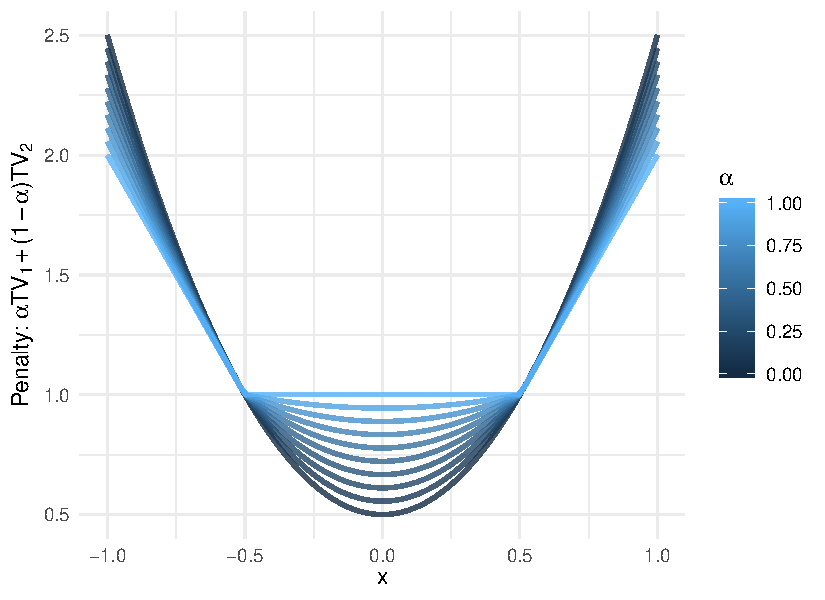
\includegraphics[width=220pt]{img/elastic-penalty.pdf}
    \caption{The figure illustrates what happens to a penalty function combining L1 and L2 total variation penalties. The function plotted here is  $f(x) := \alpha \left(|x - a| + |b - x|\right) + (1 - \alpha) \left((x - a)^2 + (b - x)^2\right)$ with varying value of $\alpha$ and $a=-1, b=1$. The figure shows that the L1 penalty is not strictly convex and has sharp corners. The L2 penalty is completely smooth and puts more mass on the interpolation point.}
    \label{fig:methods:l1-l2}
\end{figure}


\subsection{Scalable Algorithm for the GFEN}
 
 The GFEN problem \eqref{eq:gfen} can be solved at scale using a variant of the fast algorithm for the GFL presented by \citet{tansey-scott-2015} which is based on trail decompositions. A full derivation is presented in Appendix \ref{appendix:algorithm}. The central assumptions to these approach are:
 \begin{itemize}[itemsep=0pt, partopsep=0pt]
     \item The edge set $E$ can be decomposed as a non-overlapping set of trails $\mathcal{T}$. %We will assume that $\mathcal{T}$ itself can be written as a disjoint union $\mathcal{T} = \mathcal{T}_S \cup \mathcal{T}_T$ where the trails of $\mathcal{T}_S$ and $\mathcal{T}_T$ consists of spatial and temporal edges respectively. While this assumption is not strictly necessary, such construction is always possible (see appendix \ref{appendix:algorithm}) and it will be convenient for the notation.
     \item We use the ADMM algorithm \citep[see]{boyd2011distributed} to reduce the problem of smoothing over $E$ to an iterative procedure consisting of solving (in parallel) a smoothing problem en each trail regarded as a linear graph.
     \item We leverage exact linear-time solvers for each subproblem in a trail. For $p=1$ we use the method of \citet{barbero-sra-2018} and for $p=2$ the solution is given by the Kalman filter.
 \end{itemize}
 
 For ease of presentation, in this section we will focus on the case of a general graph, which corresponds to the GFEN objective \ref{eq:gfen}. The extension to the spatio-temporal case will be straightforward. In this case, it will be convenient to assume that $\mathcal{T}$ itself can be written as a disjoint union $\mathcal{T} = \mathcal{T}_S \cup \mathcal{T}_T$ where the trails of $\mathcal{T}_S$ and $\mathcal{T}_T$ consists of spatial and temporal edges respectively. This assumption is not strictly necessary, however, it simplifies computation since the total variation penalization hyper-parameters will always be constant for a given trail.
 
The first step is to rewrite the GFEN objective as a constrained optimization problem using a set of slack variables $\mathbf{z}_{\tau, p} = (z^{(v)}_{\tau, p})_{v\in \tau}$ exactly one for each trail\footnote{With a slight abuse of notation, we say that $v\in \tau$ if $v$ appears in some edge of $\tau$.} $\tau \in \mathcal{T}$ and for each norm $p\in\{1,2\}$, obtaining
\begin{equation}\label{eq:gfen-constrained}
\begin{aligned}
\operatornamewithlimits{minimize}_{\beta} \quad\quad & \sum_{v \in V} l(\mathbf{y}^{(v)}, \beta^{(v)}) + \sum_{\tau \in \mathcal{T}}  \sum_{p \in \{1,2\}} \lambda_p \mathrm{TV}_p(\mathbf{z}_{\tau, p}, \tau) \\ 
\text{subject to} \quad\;\; & \mathbf{z}_{\tau, p} = \beta[\tau] \quad\text{for all}\quad \tau \in \mathcal{T}, p \in \{1,2\}
\end{aligned}
\end{equation}
where $\beta[\tau] =  (\beta^{(v)})_{v\in \tau}$. A direct application of the ADMM algorithm \citep{boyd2011distributed} yields the following iterative updates:

\begin{equation}\label{eq:algo}
\begin{aligned}
\beta^{(v)}_{[k + 1]} &= \operatornamewithlimits{argmin}_{\beta} \; l(\mathbf{y}^{(v)}, \beta) + \alpha \sum_{\{\tau \colon v \in \tau\}} \sum_{p\in\{1,2\}} (\beta - z_{{\tau, p, [k]}}^{(v)} + u_{{\tau, p, [k]}}^{(v)})^2  & \forall v\in V \\
\mathbf{z}_{{\tau, 1, [k + 1]}} &= \operatornamewithlimits{argmin}_{\mathbf{z}} \; \lVert \mathbf{z} - \beta_{[k + 1]}[\tau] - \mathbf{u}_{{\tau, 1, [k]}}\rVert^2  + \lambda_1\mathrm{TV}_1(\mathbf{z}, \tau) \, & \forall \tau \in \mathcal{T} \\
\mathbf{z}_{{\tau, 1, [k + 1]}} &= \operatornamewithlimits{argmin}_{\mathbf{z}} \; \lVert \mathbf{z} - \beta_{[k + 1]}[\tau] - \mathbf{u}_{{\tau, 2, [k]}}\rVert^2  + \lambda_2\mathrm{TV}_2(\mathbf{z}, \tau) \, & \forall \tau \in \mathcal{T} \\
\mathbf{u}_{{t,p, [k+1]}} &= \mathbf{u}_{{t,p, [k]}} + \beta_{[k+1]}[\tau] - \mathbf{z}_{t,p, [k+1]}  \hspace{8em} \forall  p\in\{1,2\}  & \forall \tau \in \mathcal{T}
\end{aligned}
\end{equation}
where $\alpha$ is the scalar of the ADMM step-size parameter, and $\mathbf{u}_{t,p}$ are the ADMM dual variables. The algorithm depends on a random initialization of the parameters. Step 1 corresponds to a binomial negative log-likelihood model with a quadratic regularization. Following \citet{tansey-etal-2017}, we can substitute the full minimization in Step 1 a with single iteration of Newthon's method. Step 2 corresponds to the fused lasso problem for chain graphs. We leverage available linear-time solvers such as \citep{johnson-2013} and \citep{barbero-sra-2018}, which have comparative performance. We prefer the latter since it can handle different values of $\lambda_1$ for each edge, although in the current formulation it is assumed to be constant. Step 3 can be solved in linear time using the Kalman smoothing algorithm \citep[see]{welch-1995}. Finally, step 4 is the dual variable update of the ADMM algorithm in scaled form and does not require any sophisticated computation. There are different strategies to dynamically change the value $\alpha$ to accelerate convergence; empirically, we found that the method of \citet{wohlberg2017admm} worked best for our problem.

In section \ref{sec:gfl} we argued that the smoothing step can be performed in an embarrassingly parallel for every node of the tree. The algorithm above offers additional possibilities for parallelism, since steps 2-4 can be performed in parallel for each trail. In a high performance computing environment, a useful strategy would be to distribute the smoothing problem for each tree node into different computation nodes using distributed memory parallelism, while steps 2-4 can be parallelized for each trail using multi-threading, i.e., shared-memory parallelism. Multi-threading will work better if the trail decomposition used has trails of balanced lengths; see \citep{tansey-scott-2015} for a discussion on trail decomposition strategies.



 
\subsection{Choosing a Tree Splitting Scheme}

The estimated densities using a binary tree $B^{(K)}$ will assign a a constant density to every point of a leaf node $B_\gamma$. Therefore, the quality, or more precisely, the resolution, will be limited by the choice of tree. Under infinite streams of data, the depth of the tree $K$ can be increased until the leaf nodes $B_\gamma$ are very small. However, with finite data, a bad partitioning scheme might lead to poor resolution in regions of high data concentration and too much resolution on regions without likely values. To improve the construction, we suggest to use a quantile method based on the global empirical distribution formed by the aggregating the data from all the vertices. This is illustrated in figure \ref{fig:splits}, where we create quantile for the global distribution of the productivity variable in the RideAustin dataset. We will provide the details of the definition of the productivity variable in section \ref{section:case-study}. For example, with a depth $K=2$, the first splitting value would be the median, and then the bottom half would be split with the first quartile, and the top half would be split with the third quartile. More generally, for $\gamma \in \{0,1\}^k$, we can define $B_\gamma = [q_a, q_b)$ where $q_a$ and $q_b$ are global distribution quantiles corresponding respectively to $a=\sum_{j=1}^k \gamma_j 2^{-j}$ and $b=a + 2^{-k}$. This approach to splitting the output space using a balanced binary tree is commonly applied in the literature of $kd$-trees (\citet{bentley1975multidimensional}; see also \citet{brown2015building}).



\subsection{Hyper-parameter Tuning}\label{sec:hyper}

Hyper-parameter tuning can be performed using in-sample and out-of-sample criteria.
In-sample tuning for the graph-fused lasso is typically done using information criteria such as the Akaike infomration criterion (AIC) or the Bayesian information criterion (BIC) \citep{tibshirani-2015}. These methods rely on the fact the degrees of freedom are easy to compute in the graph-fused lasso, since it reduces to counting the number of plateaus \citep{tansey-scott-2015}. However, in the case of the GFEN, the L2-norm penalty adds smoothness and makes the approach of counting plateaus unfeasible. One solution that appears in the GMRF literature is to use an approximate information criterion such as the Deviance Information Criterion (DIC). However, that solution is known to favor over-fitted models and assumes an approximate normal distribution predictive distribution \citep{ando2011predictive}. Below we describe an alternative out-of-sample tuning approach based cross-validation (for a survery see \citet{arlot2010survey}).

The overall idea is that we can use $k$-cross-validation for the out-of-sample likelihood prediction. Given a set of hyper-parameters $\lambda$ for the model. We divide our data $\mathbf{y}$ into $k$ equally sized testing sets or folds $\{\mathbf{y}^{\{j\}}\}_{j=1}^k$. For each fold $j$, we use the training data $\mathbf{y}^{\{j\}}_\text{train} = \bigcup_{j' \neq j} \mathbf{y}^{\{j'\}}$ to learn the parameters of a statistical model. We then use thos parameters compute the average of the out-of-sample negative likelihood, i.e. the out-of-sample loss, using the evaluation set $\mathbf{y}^{\{j\}}_\text{test} = \mathbf{y}^{\{j\}}$. Finally, the estimate out-of-sample loss corresponding to $\theta$ is the average over all test sets $\mathbf{y}^{\{j\}}_\text{test}$. To compute the out-of-sample loss in the context of our graph density smoothing model we would to the following: for each point $y_i \in \mathbf{y}^{\{j\}}_\text{test}$, we would identify the corresponding leaf node $B(y_i)$ to which $y_i$ belongs and compute $-\log \hat{P}(y_i \in B(y_i) \mid \hat{\beta}^{\{j\}})$ using expression \eqref{eq:binomial-model} and the relevant parameters for the vertex to which $y_i$ belongs. Averaging over the losses of all the out-of-sample points for every fold we obtain the cross-validation estimate for the negative loglikelihood
\begin{equation}\label{eq:negll}
\hat{l}_\lambda := \frac{1}{N} \sum_{j=1}^k \sum_{y_i \in \mathbf{y}^{\{j\}}_\text{test}} -\log \hat{P}(y_i \in B(y_i) \mid \hat{\beta}^{\{j\}})
\end{equation}
where $N$ is the total number of data points and $\lambda$ is the vector of total variation penalization parameters. The hyper-parameters with the lowest values of $\hat{l}_\lambda$ will be preferred.

Since for a spatio-temporal GFEN we have to tune for four hyper-parameters a grid-search strategy is not recommended. For example, if we were to try 10 different values for each hyper-parameter we would then need to train $k \times 10^4 = 40,000$ models to select the best hyper-parameters using grid-search! Instead, we use a Gaussian Process \citep{snoek-etal-2012} to guide the search. The assumptions of this approach are the following:

\begin{enumerate}[itemsep=0pt, partopsep=0pt]
    \item Suppose we have observed out-of-sample losses $\hat{l}_1,\hdots, \hat{l}_n$ corresponding to hyper-parameters $\lambda_1,\hdots, \lambda_n$. The Gaussian Process assumption is that $\hat{l}_1,\hdots, \hat{l}_n$ follow a multivariate Gaussian distribution.
    \item Moreover, the multivariate distribution is assumed to have the following form
    $$
    (\hat{l}_1,...,\hat{l}_n)  \sim \mathrm{Normal}(0, K + \sigma^2 I), 
    $$
    where $K:=(K_{ij})_{i,j=1}^n$ is some Kernel matrix depending on $\lambda_1,\hdots,\lambda_n$ and $\sigma^2$ models the uncertainty in the observations $\hat{l}_j$. A typical example of kernel matrix $K$ is the radial kernel $K_{ij}=\exp(-a \lVert \lambda_i - \lambda_j\rVert^2_2)$ where $a$ controls the degree of correlation between similar hyperparamters.
    \item Given a new point $l_*$ corresponding to an untested hyper-parameter $\lambda_*$, the fact that $(l_*, \hat{l}_1,\hdots, \hat{l}_n)$ is multivariate Gaussian can be used to easily compute the predictive mean value of $l_*$ given the observed $\hat{l}_1,\hdots, \hat{l}_n$. More precisely, given a series of candidate untested hyper-parameters, we select the $\lambda_*$ that has the lowest expected loss $E[l_* \mid \hat{l}_1,\hdots, \hat{l}_n]$.
\end{enumerate}
The above steps give a high-level description of the idea of Bayesian optimization. For a detailed explanation we refer the reader to the review by \citet{shahriari-etal-2016}. In section \ref{section:case-study} we will provide additional details about our implementation for the RideAustin dataset.

% We proceed in generations; in each step, we use the current estimate of the predictive distribution to generate a sample of hyperparameters with small predicted out-of-sample loss. After we repeat the inference procedures with the new combinations of hyperparameters and estimate the new out-of-sample losses, we update our posterior predictive using Bayesian inference. In our case, 10 generations of size 16 worked well. Note that the procedures within each generation can be embarrassingly parallelized.




\section{Simulations}\label{section:simulation}

We conducted a series of experiments to better understand how the GFEN compares with respect to the GFL and a GMRF. 

\subsection{Visualization of the GFEN}

We first look at the problem of estimating a one-dimensional signal. This would correspond to the case when the likelihood term in expression \eqref{eq:gfl} is a quadratic error, which can be interpreted as coming from a Normal distribution. Figure \ref{fig:benchmarks-linear} shows the comparison of the best fitted values for the GFL, GFEN and GMRF for synthetic data that consists of a true signal which is a mix of locally constant and smooth transitions, on a chain graph of $N=150$ vertices. The data from the simulated signal is observed with noise and with $p_\text{miss}=2/3$ of the vertices having missing data. Since the GFL is not well-defined with missing data (see section \ref{subsection:gfl-non-convex}), a small quadratic shrinking penalty was added. The hyper-parameter values for the smoothing were selected using cross-validation for minimizing the out-of-sample quadratic error, similar to the procedure explained in section \ref{sec:hyper}. We can observe in the figure that the GFEN has an intermediate behavior between the GFL and the GMRF. The recovered signal is mostly locally constant for the part of the signal which is flat, and becomes smooth for the last third of the signal which is linear behaving more similar to the GMRF estimate. We also notice that it interpolated between nodes 50 and 60 where there is no data, just as the GMRF, whereas the GFL estimate are shrunk towards the origin. In general, the GFEN estimate is less wiggly than its GMRF counterpart.

\begin{figure}[tb]
    \centering
    \begin{subfigure}[tb]{.3\linewidth}
        \centering
        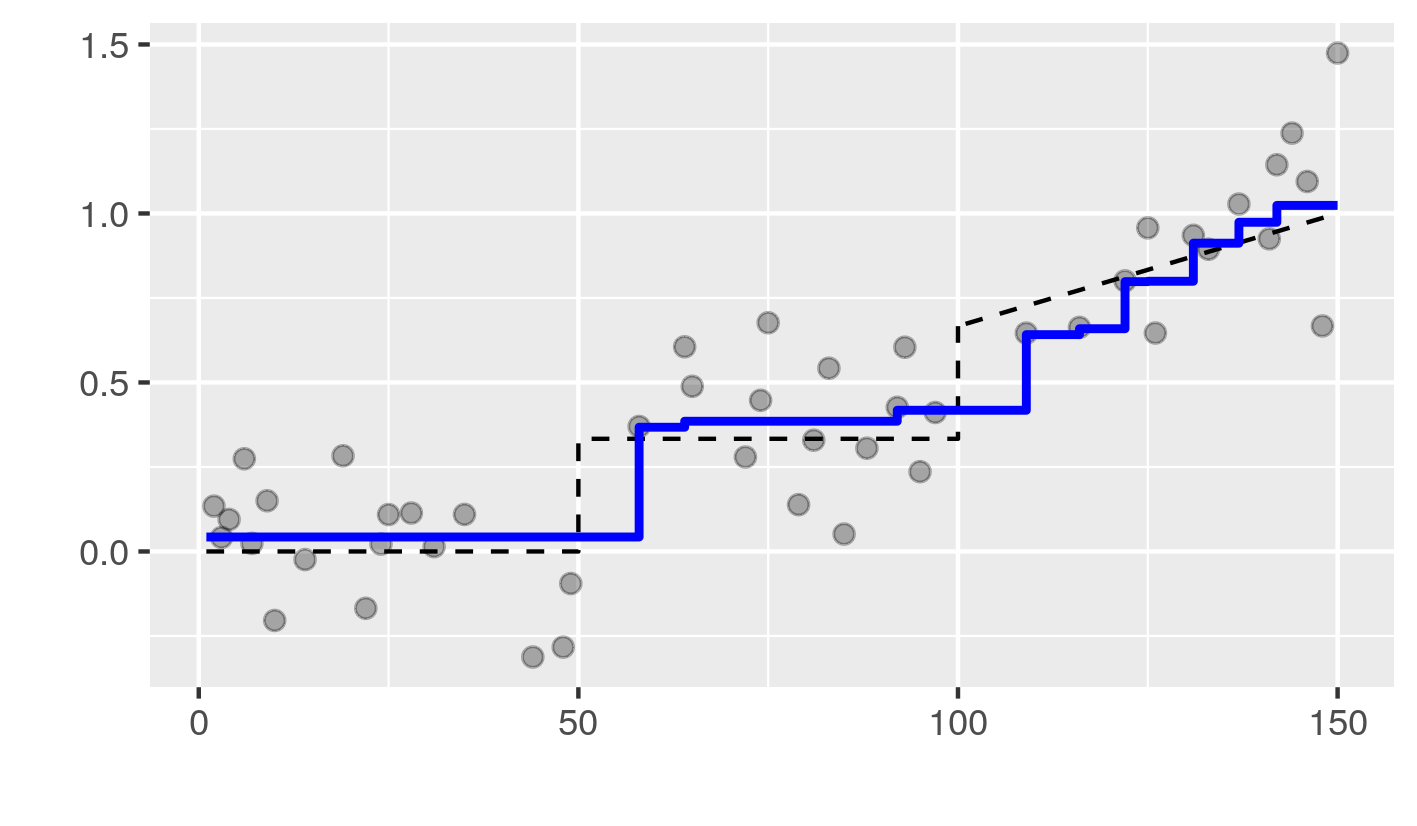
\includegraphics[width=0.98\linewidth, height=100px]{img/benchmarks_linear_fl.png}
        \caption{\footnotesize GFL}
        % \label{fig:prod:spatial}
    \end{subfigure}%
    ~
    \begin{subfigure}[tb]{.3\linewidth}
        \centering
        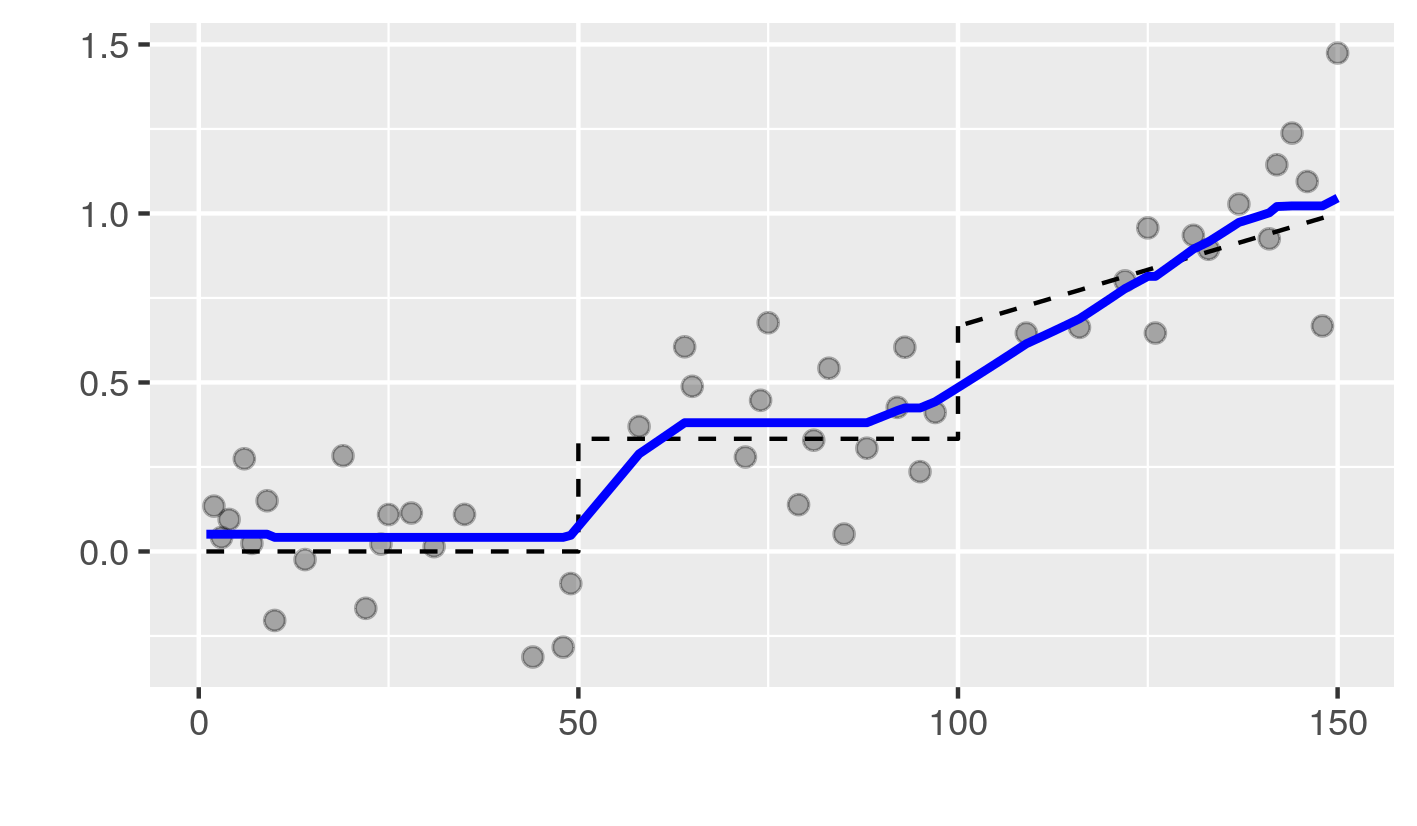
\includegraphics[width=0.98\linewidth, height=100px]{img/benchmarks_linear_enet.png}
        \caption{GFEN}
        % \label{fig:prod:timely}
    \end{subfigure}
    ~
    \begin{subfigure}[tb]{.3\linewidth}
        \centering
        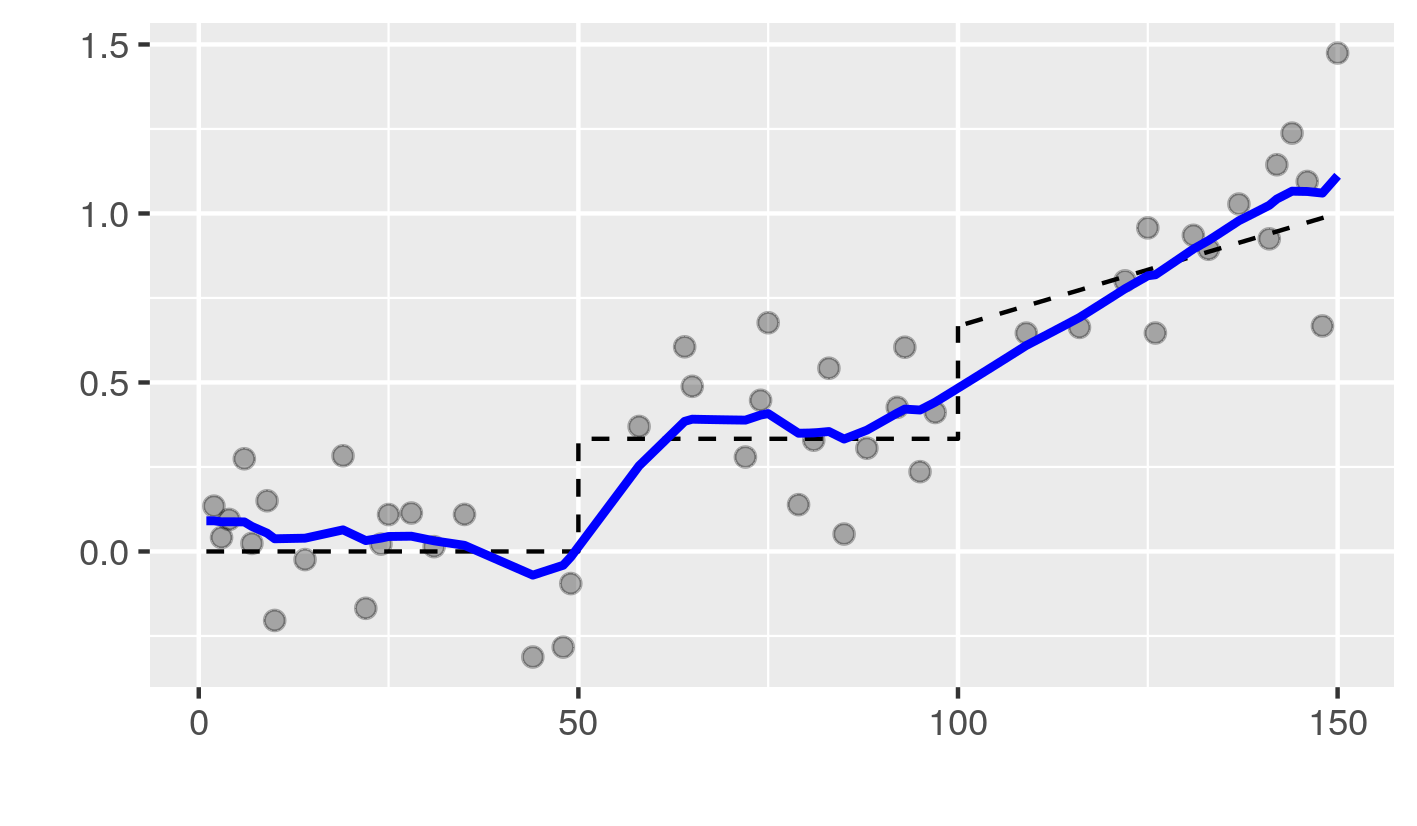
\includegraphics[width=0.98\linewidth, height=100px]{img/benchmarks_linear_kal.png}
        \caption{\footnotesize GMRF}
        % \label{fig:prod:spatial}
    \end{subfigure}%
    \caption{Comparison of methods on the estimation of a signal on a chain graph of size $N=150$. The true signal (dashed) is a mix of discontinuous locally constant and smooth transitions. Data is observed with noise with two thirds of the vertices having missing data. The GFL (left) does a good job at estimating locally constant part of the signal. Since a quadratic shrinking penalty was added to the GFL to ensure the problem is strictly convex due to the missing data, regions with missing observations are shrunk towards the origin to the closer value with data. The GMRF estimates a smoother signal but with more wiggling, even in the locally constant region. The behavior of the GFEN is intermediate between the other two, being locally constant and smooth in the corresponding regions of the true signal, and interpolating in regions with missing data.} 
    \label{fig:benchmarks-linear}
\end{figure}

We now look at the problem of density estimation using the binary tree strategy described in section \ref{section:methodology}. This is shown in Figure \ref{fig:benchmarks-density}. The densities trying to be estimated our mixtures of Gaussian with fixed standard deviation. The mean of each Normal component is shifted according to along a chain graph of $N=150$ and follows a transition similar to the one shown for the signal estimation case earlier. More precisely, the mean of each component is constant for the first two-thirds of the graph with a discontinuity in between, and linearly smooth in the last third. Moreover, two thirds of the vertices have missing data, in the rest we observe 10 samples from the true distribution. The vertex position and the number of samples are shown for each density estimate at each vertex. The hyper-parameters are selected to maximize the cross-validated out-of-sample likelihood. In the figure we can observe that the GFL gives yield bad estimates for the regions of missing data in vertices 40-60 and 90-110. The GFEN yields spikier density estimates than the GFEN, although this is harder to observe. In what follows we provide a more systematic way to compare the different approaches.

\begin{figure}[tb]
    \centering
    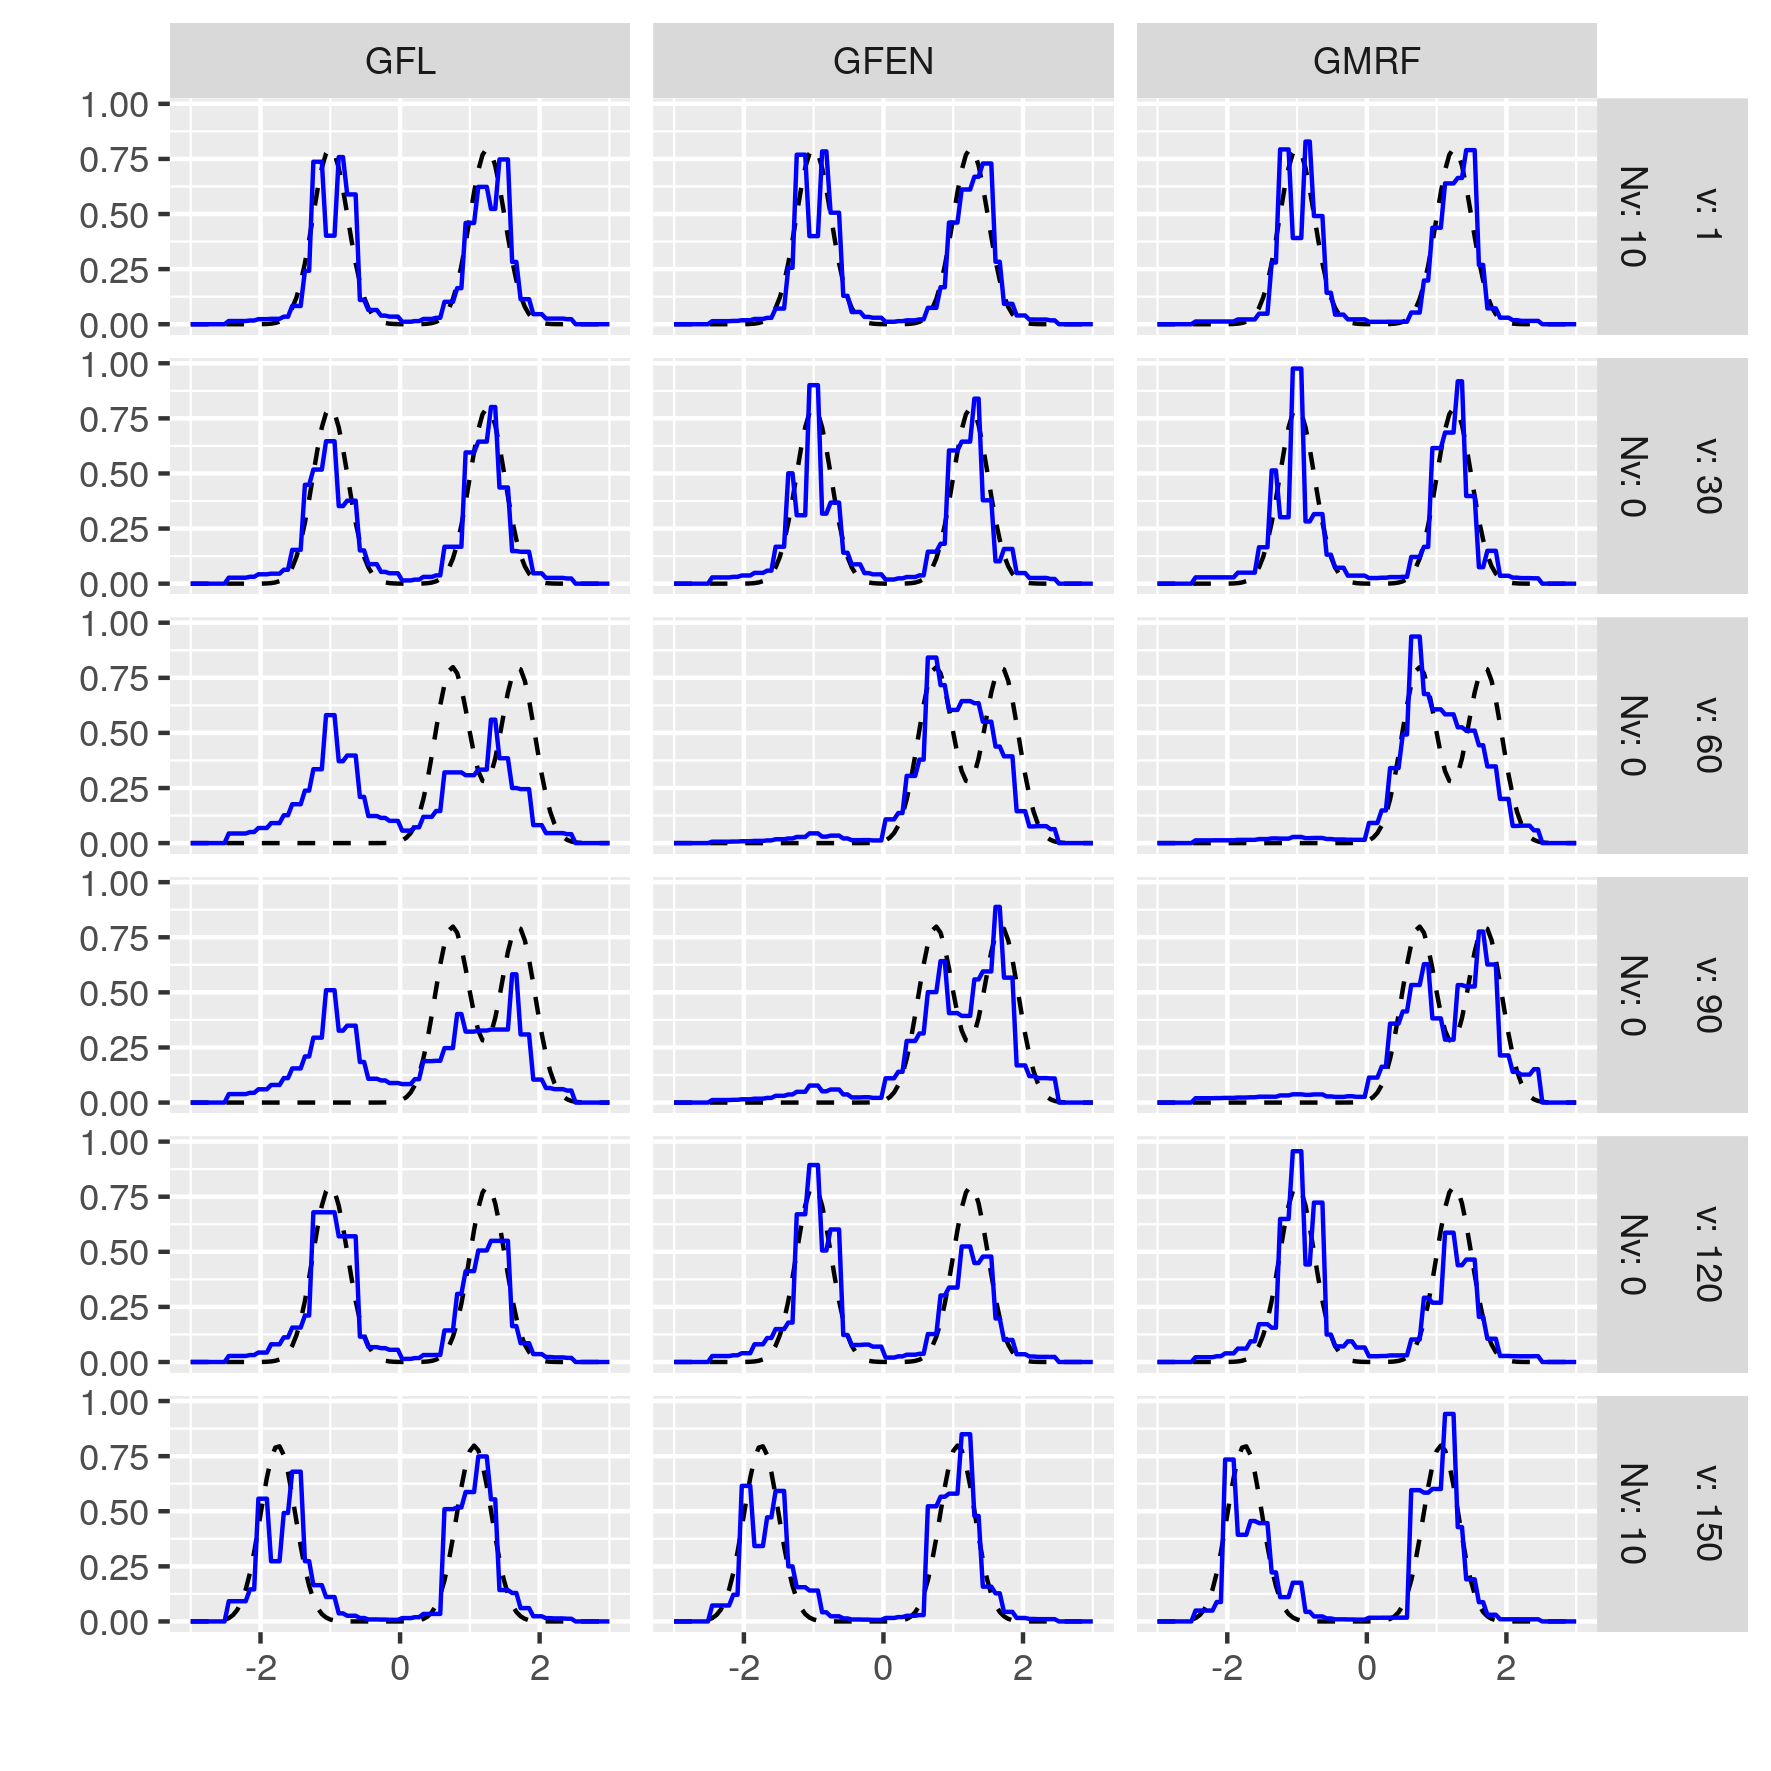
\includegraphics[width=11cm, height=10cm]{img/benchmarks_densities_vertical.png}
    \caption{Comparison of the estimation of a density using a binary tree of depth $K=5$ on a chain graph of size $N=150$. Estimates are shown at vertices $v=1, 30, 60, 90, 120, 150$ (vertical axis) and for each method (horizontal axis). The true densities are mixtures of Gaussians with varying means (dashed). At each vertex a sample of size $N_v=10$ from the true distributions is observed. Except at vertices 40-60 and 90-110 which have missing data, as well as other scattered vertices for a total of a two thirds of missing data ($N_v=0$). GFL performs poorly in the large patches without data (40-60 and 90-110), whereas GFEN and GMRF perform better, although the latter is more spiky. Parameters are selected by cross-validation with negative loglikelihood.} 
    \label{fig:benchmarks-density}
\end{figure}

% \begin{figure}[tb]
%     \centering
%     \begin{subfigure}[tb]{0.95\linewidth}
%         \centering
%         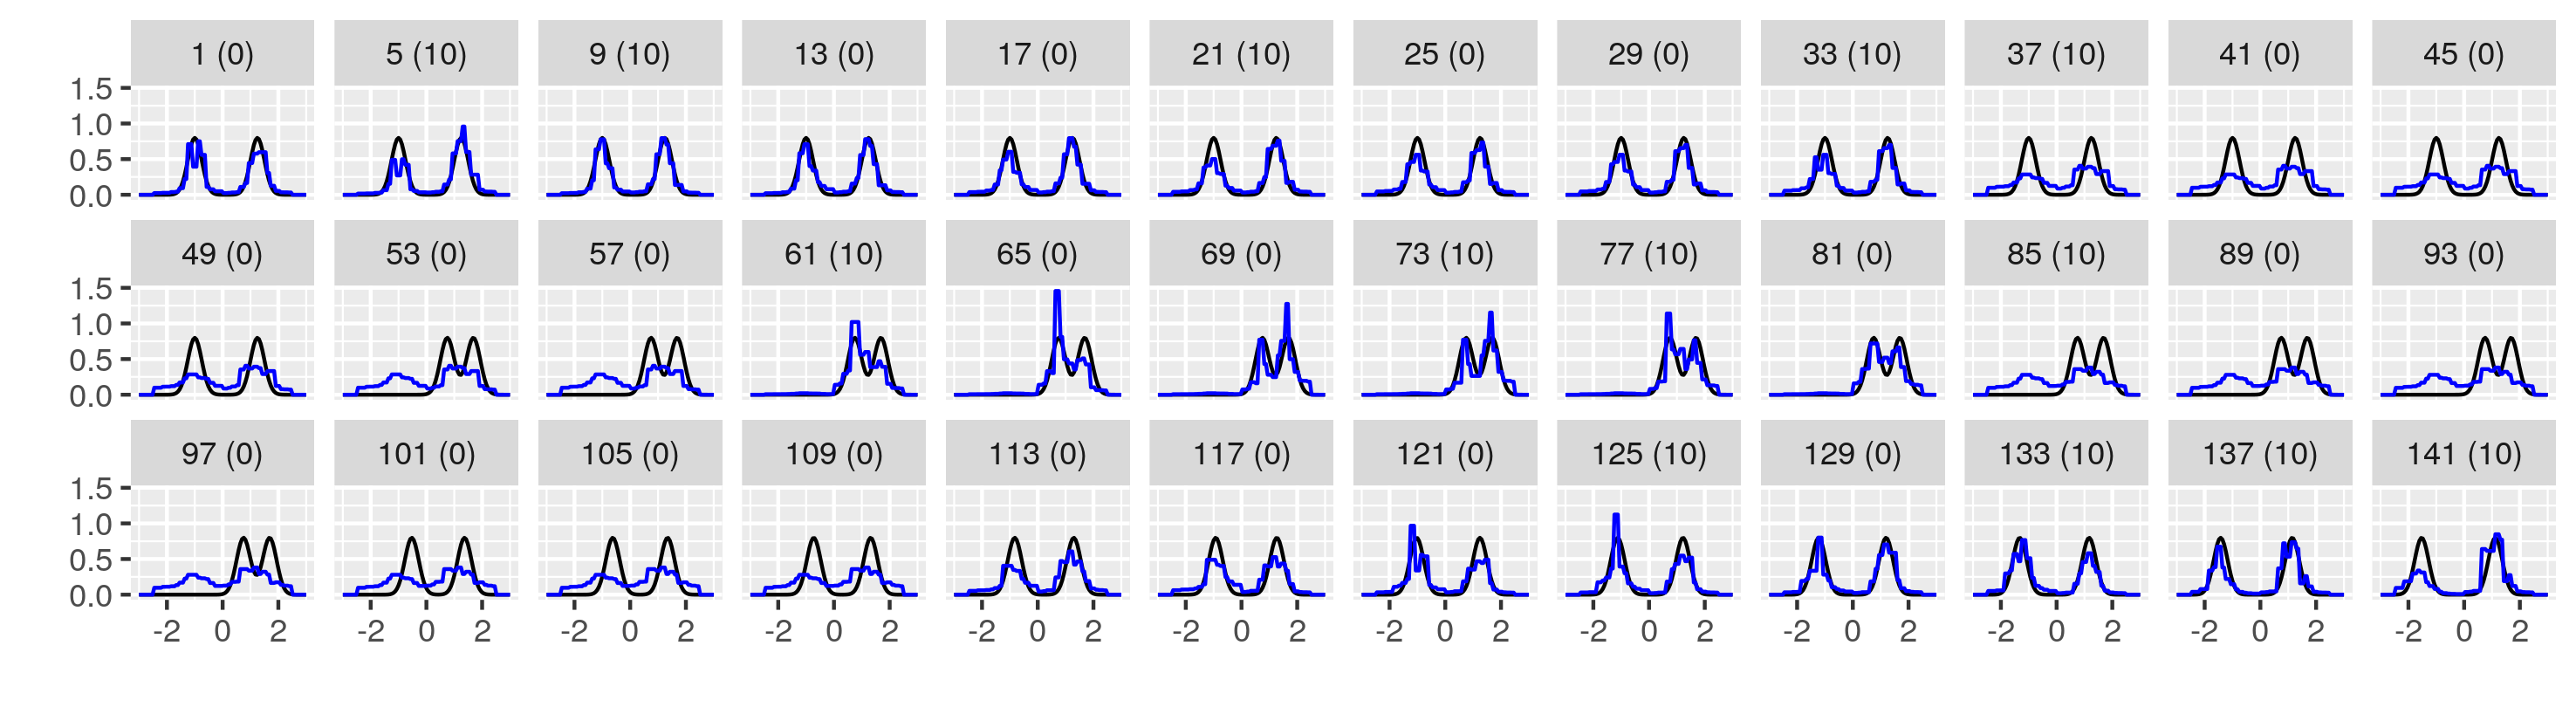
\includegraphics[height=3.2cm, width=0.95\linewidth, trim={0 0.9cm 0 0}]{img/benchmarks_densities_fl.png}
%         \caption{Graph-fused lasso (GFL)}
%         % \label{fig:prod:timely}
%     \end{subfigure}   \hfill\\
%     \begin{subfigure}[tb]{0.95\linewidth}
%         \centering
%         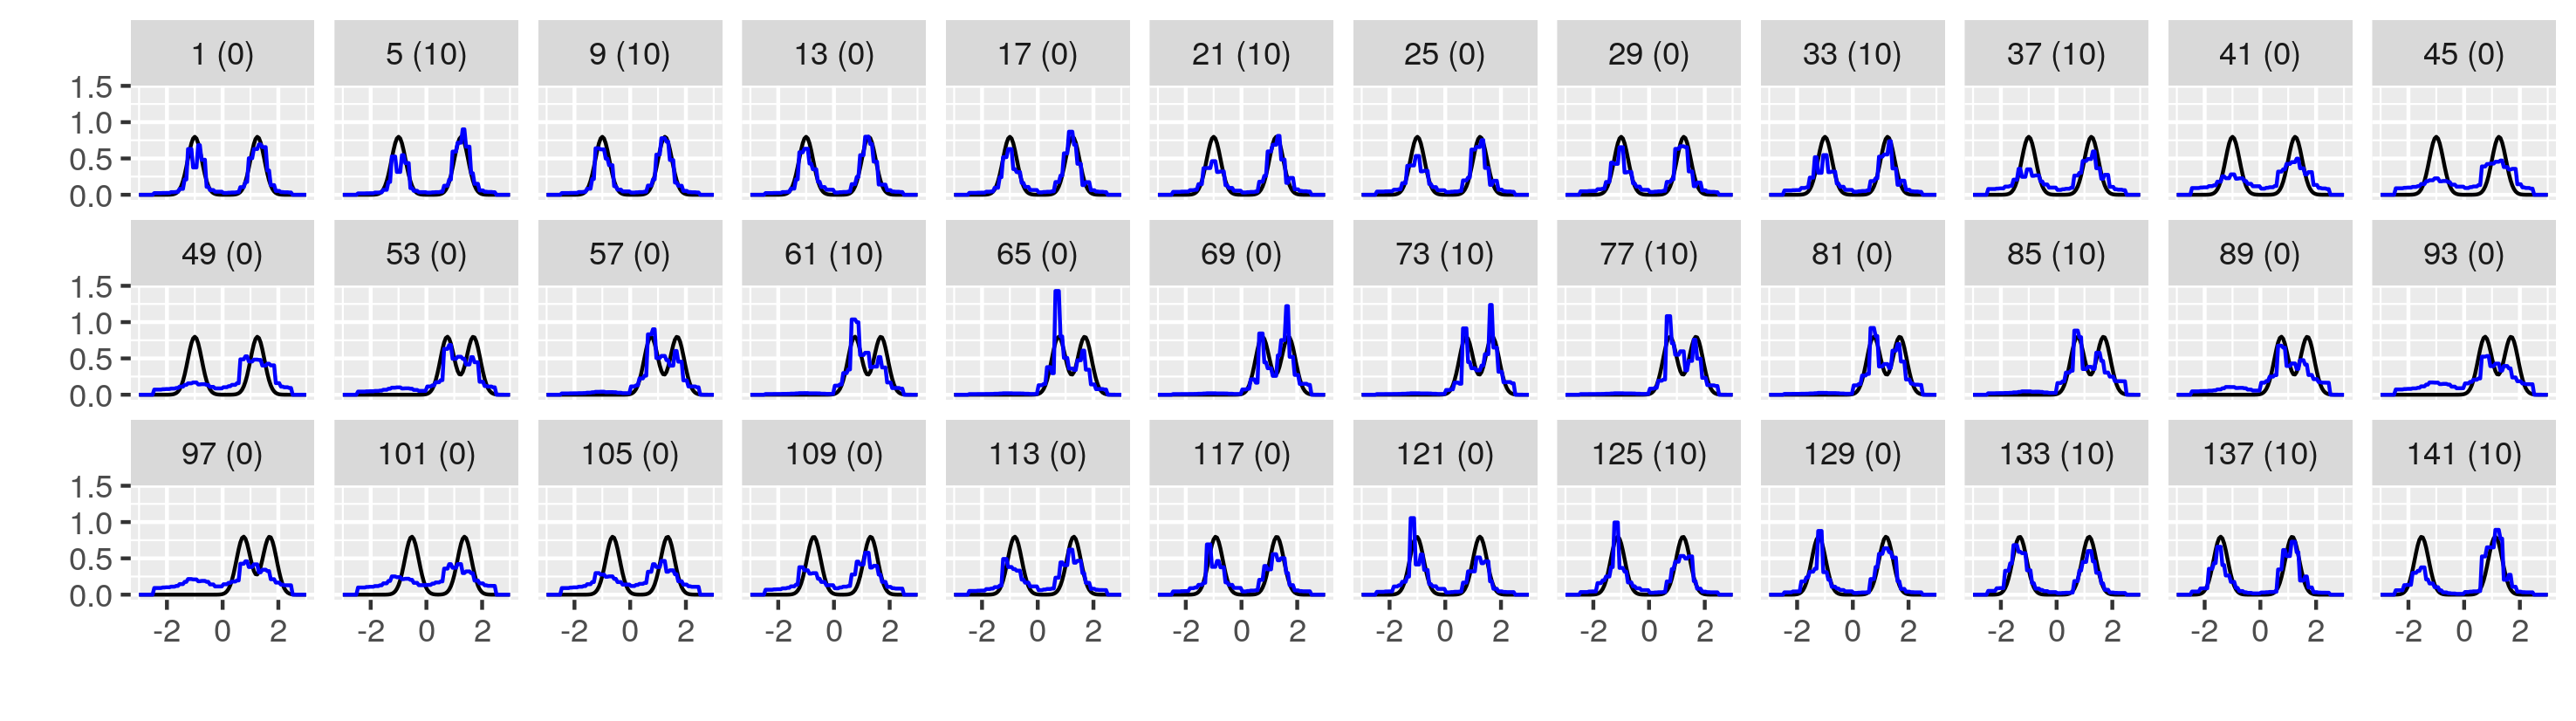
\includegraphics[height=3.2cm, width=0.95\linewidth, trim={0 0.9cm 0 0}]{img/benchmarks_densities_enet.png}
%         \caption{Graph-fused elastic net (GFEN)}
%         % \label{fig:prod:spatial}
%     \end{subfigure}   \hfill \\
%     \begin{subfigure}[tb]{0.95\linewidth}
%         \centering
%         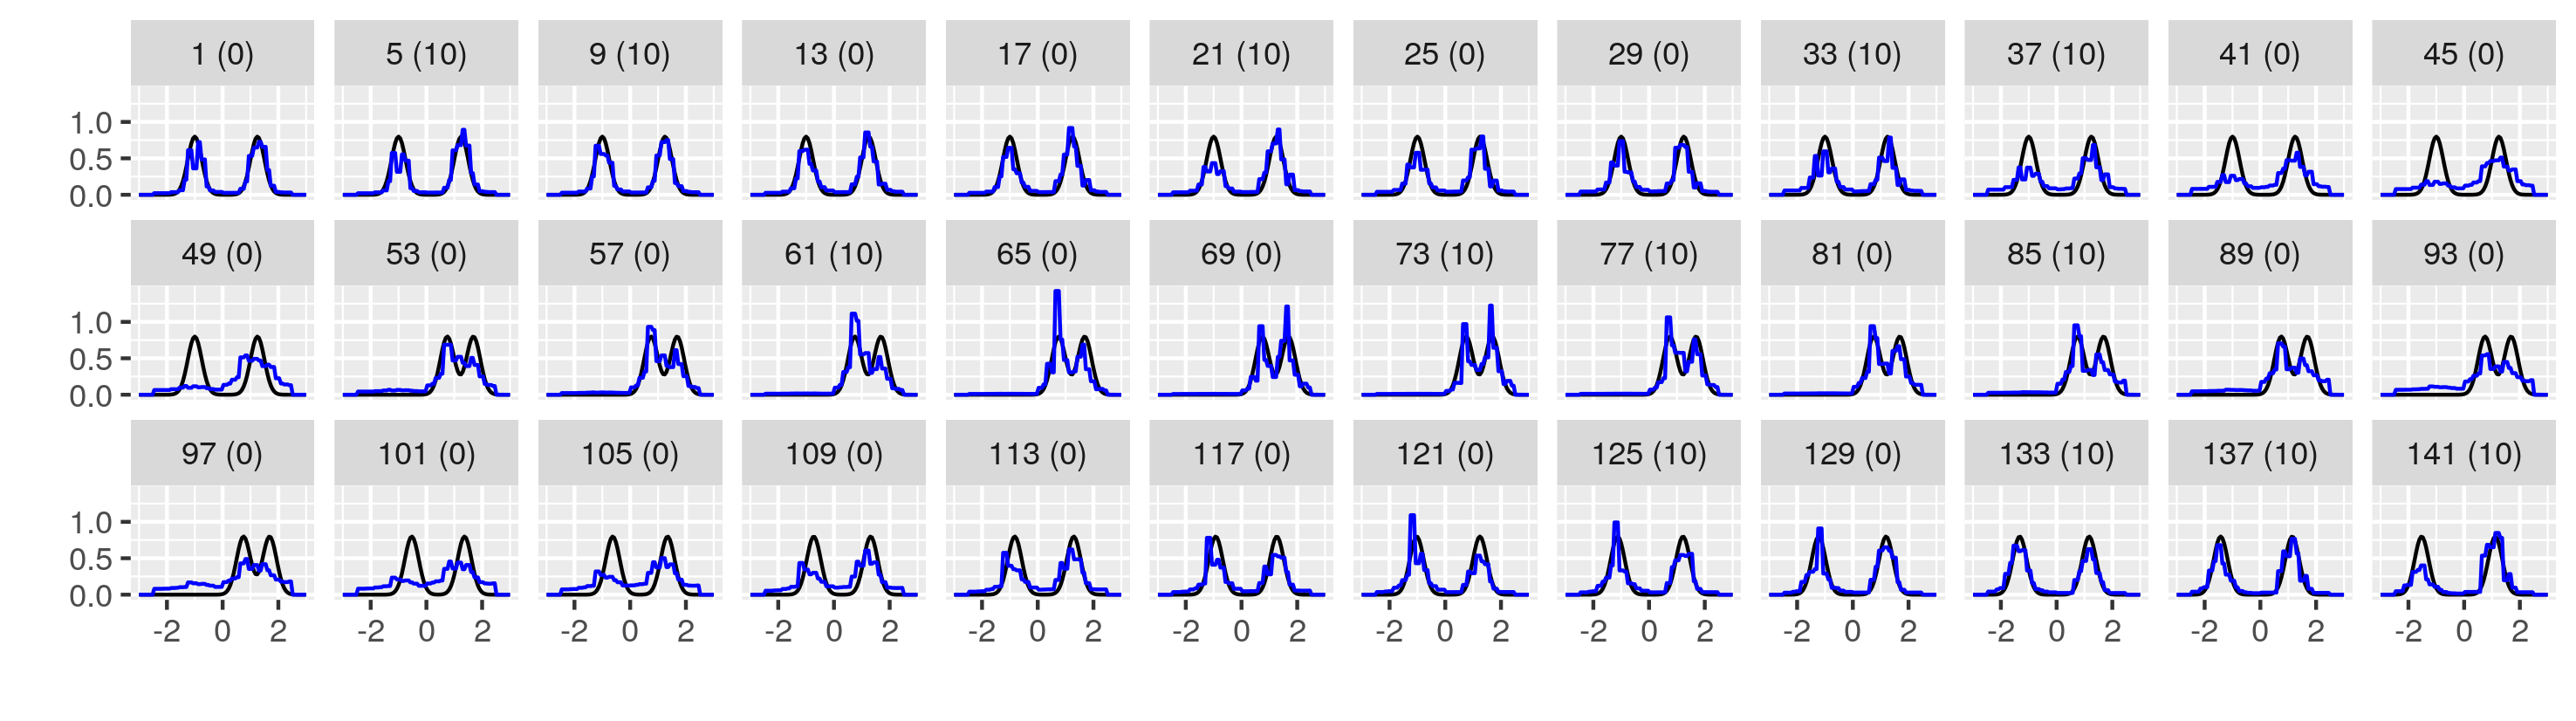
\includegraphics[height=3.2cm, width=0.95\linewidth, trim={0 0.9cm 0 0}]{img/benchmarks_densities_kal.png}
%         \caption{Gaussian Markov Random Field (GMRF)}
%         % \label{fig:prod:spatial}
%     \end{subfigure}%
%     \caption{Comparison of the estimation of a density using a binary tree of depth $K=5$ on a chain graph of size $N=150$. The densities are mixtures of Gaussians with varying means. The true distribution is shown in black, and the fitted in blue. The mean of each component changes according to a mix of piece-wise constant and smooth transitions. The vertices 40-60 and 90-110 have missing data. Other scattered vertices have also missing data for a total of two thirds of the vertices, and the rest have 10 observations from the true distribution. The available data is shown in parenthesis next to the vertex position. GFL performs poorly in regions without data (40-60 and 90-110). GFEN and GMRF are quite similar, although the latter is a bit more spiky.} 
%     \label{fig:benchmarks-density}
% \end{figure}

\subsection{Comparison Simulation Tasks}

Building on the scenario of mixtures of Gaussians shown in Figure \ref{fig:benchmarks-density} and discussed in the earlier section, we designed four density estimation tasks. For each task we simulated a 100 datasets for chain graph data and compared distinct metrics about the quality of the fitted distributions averaged across all vertices. The distributions are fitted using a binary tree of depth $K=5$. We now provide a high-level description of each task and metric. Technical details about the construction of the datasets are provided in appendix \ref{appendix:sim-data}. The four tasks are based on density estimation of a mixture of Gaussians with two components with shifting mean and fixed variance. The four variants are
\begin{enumerate}[itemsep=0pt, partopsep=0pt]
    \item \textbf{piecewise-constant}. The component of each mean follows a locally constant process with two discontinuities. The values of the plateaus and the discontinuity positions are chosen at random.
    \item \textbf{smooth}. Instead of two discontinuities. The trajectory of the shifting means is continuous and piecewise-linear with the values of the values with two slope changes chose at random in value and position in the graph.
    \item \textbf{mixed}. Combines the two above tasks. Now the trajectories are a combination of piece-wise constant and piece-wise linear (smooth). To do so, the trajectory is divided in three segments of random size, and each segment is randomly assigned to be locally constant or piece-wise smooth.
    \item \textbf{mixed+outliers}. It produces a true distribution similar to the mixed case, but we one outlier to some of the vertices. This outlier is chose to come from a contaminating distribution of five times the typical standard deviation. This approach could be seen as a third mixture component, however, we prefer to think of it as corrupt measurement.
\end{enumerate}
In addition, each task will be evaluated under a regime of $p_\text{miss}=10\%$ vertices with missing data and of $p_\text{miss}=80\%$ vertices with missing data. A priori, we expect the GFL to work best in the piecewise-constant task, particularly with low missing data. Conversely, the GMRF should work best for the smooth task. The GFEN should have a balanced performance, being best for the mixed task. The metrics that we will use to evaluate the performance are:
\begin{enumerate}[itemsep=0pt, partopsep=0pt]
    \item \textbf{out-of-sample negative loglikelihood (negll)}. This is the cross-validation negative loglikelihood that is used to select the best hyper-parameters using expression \eqref{eq:negll}. 
    \item \textbf{mean root integrated squared error (mrise)}. The root integrated squared error is defined as $$\mathrm{rise}(\hat{p}) = \left(\int (p(x) - \hat{p}(x))^2 dx\right)^{1/2}$$ where $p(x)$ and $\hat{p}(x)$ are the true and estimated densities. We estimate the rise for each vertex of the graph and average the estimations to obtain the mrise.
    \item \textbf{mean integrated absolute mean error (miae)}. The metric is very similar, but instead we use the integrated absolute error
    $$
    \mathrm{iae}(\hat{p}) = \int \left| p(x) - \hat{p}(x)\right| dx
    $$
    and the average over all vertices to obtain the miae.
\end{enumerate}
The main difference between the \textit{rise} and \textit{ise} metrics is that the former penalizes more larger differences. The rise and ise correspond do the L1 and L2 metrics in functional space. To evaluate them we use standard numerical integration methods.

\subsection{Results}

Table \ref{tab:benchmarks} shows the results. The GFEN is expected to always be the minimizer of the negll, since the GFL and the GMRF as special cases of the GFEN, so there is always a combination parameters that is as good or better, and the negll was used for the hyper-parameter selection. The only reason why it is not always the best is because the hyper-parameter search might not always be fully successful. The mrise tells a different story. It shows that the GFL is the best performer for the piecewise-constant case, and the GMRF for the smooth case, but each are the worst performers for the other case. The GFEN on the contrary, is overall always a good performer and it is the best for the mixed data case, with or without outliers. Another interesting point to highlight is that the GFL is generally better with respect to the absolute error and to the squared error metric. We can conclude this section pointing out that the GFEN perform good for mixed effects, as the ones we an expect for the RideAustin data.

\begin{table}[tb]
    \centering
    % \ra{0.95}
    \small
    \begin{subtable}[b]{.4\linewidth}
      \centering
      \begin{tabular}{l|c|c|c}
         method & negll & mrise & miae \\ \midrule
         GFL  & 2.86 & \textbf{1.26} &  \textbf{1.23} \\ 
         GMRF & 1.63 & 2.75 &  2.66 \\ 
         GFEN & \textbf{1.50} & 2.10 &  2.10  \\ 
     \end{tabular}
     \caption{piece-wise constant, $p_\text{miss} = 0.1$}
    \end{subtable}%
    ~
    \begin{subtable}[b]{.4\linewidth}
      \centering
      \begin{tabular}{l|c|c|c}
         method & negll & mrise & miae \\ \midrule
         GFL & 1.71 & \textbf{1.35} & \textbf{1.17} \\ 
         GMRF & 2.89 & 2.75 & 2.97 \\ 
         GFEN & \textbf{1.40} & 1.91 & 1.86 \\ 
     \end{tabular}
     \caption{piece-wise constant, $p_\text{miss} = 0.8$}
    \end{subtable}\vspace{10px}\\
    % \vspace{10px}
    \begin{subtable}[b]{.4\linewidth}
      \centering
      \begin{tabular}{l|c|c|c}
        %  method & negll & mrise & miae \\ \midrule
         GFL &  2.83 & \textbf{1.43} & \textbf{1.43} \\ 
         GMRF & 1.66 & 2.33 & 2.33 \\ 
         GFEN & \textbf{1.5}  & 2.33 & 2.33\\ 
      \end{tabular}
     \caption{smooth, $p_\text{miss} = 0.1$}
    \end{subtable}%
    ~
    \begin{subtable}[b]{.4\linewidth}
      \centering
      \begin{tabular}{l|c|c|c}
        %  method & negll & mrise & miae \\ \midrule
         GFL & 2.87 & 2.99 & 1.88 \\ 
         GMRF & 1.92 & \textbf{1.42} &  2.48 \\ 
         GFEN & \textbf{1.21} & 1.59 & \textbf{1.64} \\ 
      \end{tabular}
     \caption{smooth, $p_\text{miss} = 0.8$}
    \end{subtable}\vspace{10px}\\
    \begin{subtable}[b]{.4\linewidth}
      \centering
      \begin{tabular}{l|c|c|c}
        %  method & negll & mrise & miae \\ \midrule
         GFL & 2.83 & \textbf{1.50} & \textbf{1.56} \\ 
         GMRF & 1.66 & 2.60 & 2.60 \\ 
         GFEN & \textbf{1.50} & 1.90 & 1.83 \\ 
      \end{tabular}
     \caption{mixed, $p_\text{miss} = 0.1$}
    \end{subtable}%
    ~
    \begin{subtable}[b]{.4\linewidth}
      \centering
      \begin{tabular}{l|c|c|c}
        %  method & negll & mrise & miae \\ \midrule
         GFL & 2.39 & 2.44 & \textbf{1.35} \\ 
         GMRF &  2.35  & 1.98  & 2.83 \\ 
         GFEN & \textbf{1.26} & \textbf{1.58} & 1.82 \\ 
      \end{tabular}
     \caption{mixed, $p_\text{miss} = 0.8$}
    \end{subtable}\vspace{10px}\\
    % \vspace{10px}
    \begin{subtable}[b]{.4\linewidth}
      \centering
      \begin{tabular}{l|c|c|c}
        %  method & negll & mrise & miae \\ \midrule
         GFL & 2.46 & \textbf{1.46} & \textbf{1.43} \\ 
         GMRF & 2.06 & 2.46 & 2.46 \\ 
         GFEN & \textbf{1.46} & 2.06 & 2.10 \\ 
      \end{tabular}
     \caption{mixed+outliers, $p_\text{miss} = 0.1$}
    \end{subtable}%
    ~
    \begin{subtable}[b]{.4\linewidth}
      \centering
      \begin{tabular}{l|c|c|c}
        %  method & negll & mrise & miae \\ \midrule
         GFL & 1.90 & 2.10 & 2.10 \\ 
         GMRF &  2.20  & 2.40  & 2.40 \\ 
         GFEN & \textbf{1.9} & \textbf{1.5} & \textbf{1.50} \\ 
      \end{tabular}
     \caption{mixed+outliers, $p_\text{miss} = 0.8$}
    \end{subtable}%
    \caption{Performance comparison on density estimation tasks of two-component mixtures of Gaussians on chain graphs with different shifting dynamics of the means. The table shows the mean rank among all 100 experiments: where 1 is the best performer and 3 is the worst performer. The best hyper-parameters for each method are chosen using cross-validation for the out-of-sample negative loglikelihood (negll). The other metrics shown are the root mean integrated squared error (mrise) and the mean integrated absolute error (miae) with respect to to the true density. GFL tends to be the best performer in all tasks for the low missing data scenario, but in the high missing data scenario it is only better when the true signal is piece-wise constant. The GFEN is overall a good performer and best for the mixed task.} 
    \label{tab:benchmarks}
\end{table}


% \begin{figure}[tb]
%     \centering
%     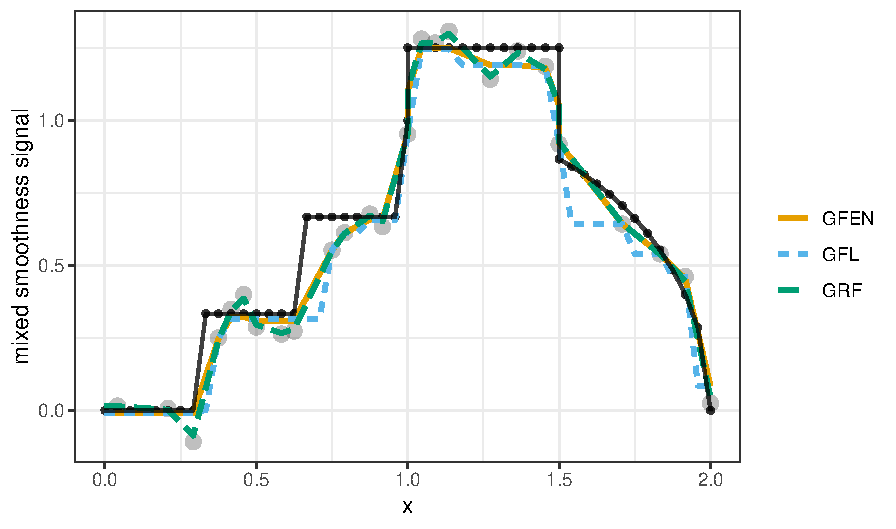
\includegraphics[width=350pt]{img/comparison_example_filter.pdf}
%     \caption{The figure shows a comparison of the Graph-fused Elastic Net (GFEN) ($\lambda_1 = 0.05, \lambda_2=0.05$), the Graph-fused Lasso (GFL) ($\lambda=0.06$) and a Gaussian Random Field (GRF) ($\lambda=0.1$). The true signal is shown with a black line. The observed data is shown with gray markers which has 50\% missing data from the original signal and is observed with Gaussian noise. Since the GFL is not well-defined a small quadratic penalty on the coefficients was added, which causes the GFL estimate to be shrinked towards the origin (see section \ref{subsection:gfl-non-convex}). It performs worst on the last bit of the signal which is smoother. The GRF, which is the Kalman filter, better captures the smoothness but it is more wiggly and is affected by big jumps. GFEN sits in between, being more robust than the GRF and better behaved with smoothness and missing data than the GFL.}
%     \label{fig:comparison:example-filter}
% \end{figure}



\section{Case study: Driver Productivity Analysis}
\label{section:case-study}


\subsection{Ride-sourcing data}

The non-profit TNC \textit{RideAustin}, based in Austin, Texas, published data about their ride-sourcing service in early 2017 \citep{dataworld-2017}. The dataset records rides the happened between June 2nd, 2016 and April 13th, 2017. Each trip corresponds to a row in the database and includes information about origin and destination coordinates, starting and ending time, driver number, cost and request time. During this period \textit{RideAustin} had no major competition, since rival companies such as Uber and Lyft were temporarily restricted from operating in Austin.

Since the demand during the first month was limited, we restricted our analysis on data from September 1st, 2016 to April 13th, 2017. We selected rides having origin and destination coordinates within the traffic analysis zones (TAZs) of Austin. 

Since a trip can have different car categories and rates (examples of car categories are regular, SUV, and premium), in order to make every trip comparable, we standardized all of them to the regular car category using RideAustin's public pricing formula. We did the same thing to remove the surge price from some trips. Our motivation for removing the surge price is that whereas the pricing scheme is known and dependent on standard features such as mileage and time rates, the surge price onset and offset is less predictable. We use the same standardizing process describe by \citet{zuniga-etal-2019}.

\subsection{Measuring productivity}\label{subsection:productivity}

To measure driver productivity, we follow \citet{zuniga-etal-2019}. We recall the approach now. Our \textit{productivity} measurement is taken \textit{prospectively} from the driver's future rides. For each trip $i$, we denote:
\begin{itemize}\itemsep0em 
    \item $\mathtt{idle}_i$: the time in hours that the driver of trip $i$ will wait until beginning a subsequent trip; during this time the driver does not generate any revenue.
    \item $\mathtt{durnext}_i$: the time in hours that the \underline{same driver} of trip $i$ will take to complete the subsequent trip; during this time the driver is generating revenue determined by the tariff system.
    \item $\mathtt{farenext}_i$: the final fare of the subsequent trip; it is a function of a distance and a time tariff rate; \textit{c.f.} \citep{zuniga-etal-2018} for more details.
\end{itemize}

Our variable of interest is then defined as 
\begin{equation}
    \label{eq:productivity-def}
    \mathtt{productivity}_i := \frac{\mathtt{farenext}_i}{\mathtt{idle}_i + \mathtt{durnext}_i}
\end{equation}
Expression \eqref{eq:productivity-def} yields an interesting definition of productivity because it combines the time that the driver will stay unproductive with the quality of the subsequent trips. Moreover, its values are given naturally in dollars/hour. The idea is that when a trip ends, the driver starts searching for new riders. This prospective measurement gives the expected earnings given that a driver is at the specific location and time at which the last trip ended. If a trip ends in a location of low demand, the idle time will be large, but also subsequent trips could be longer. We remark that this definition deliberately ignores the fare trip that led to that position.

\begin{figure}[tb]
    \centering
    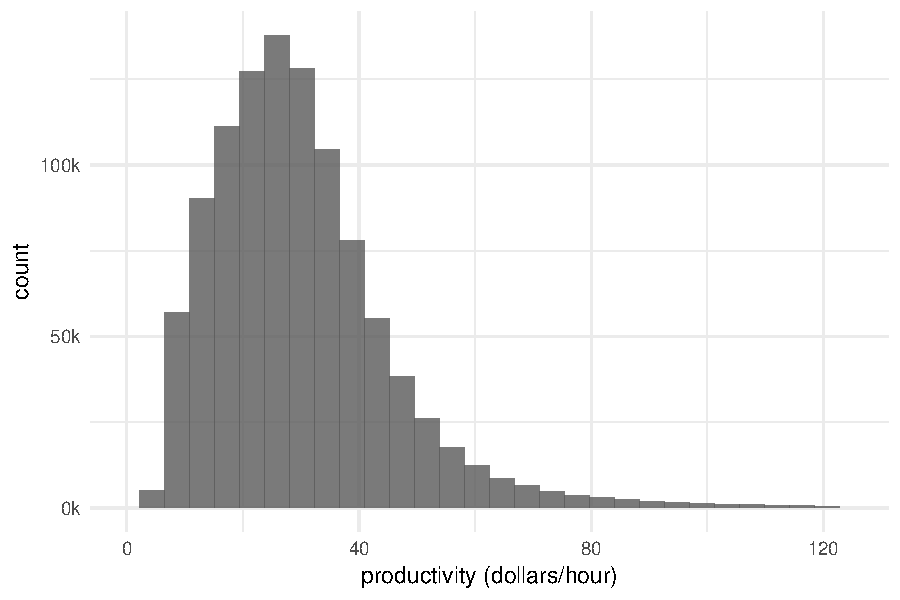
\includegraphics[width=0.65\linewidth]{img/prodhist_global.pdf}
    \caption{Histogram of productivity considering all trips}
    \label{fig:prodhist}
\end{figure}

We only considered trips in which the waiting time for a subsequent trip was less than one hour. This was necessary in order to exclude the cases where the driver took a break or stopped working for the day. Since during the time of data collection RideAustin did not have a major competing company, we do not have problems with long inter-trip times due to app switching. Figure \ref{fig:idledist} shows the distribution of the idle time in between trips after preprocessing and its distribution across TAZs.


\begin{figure}[tb]
    \centering
    \begin{minipage}[tb]{.8\linewidth}
        \centering
        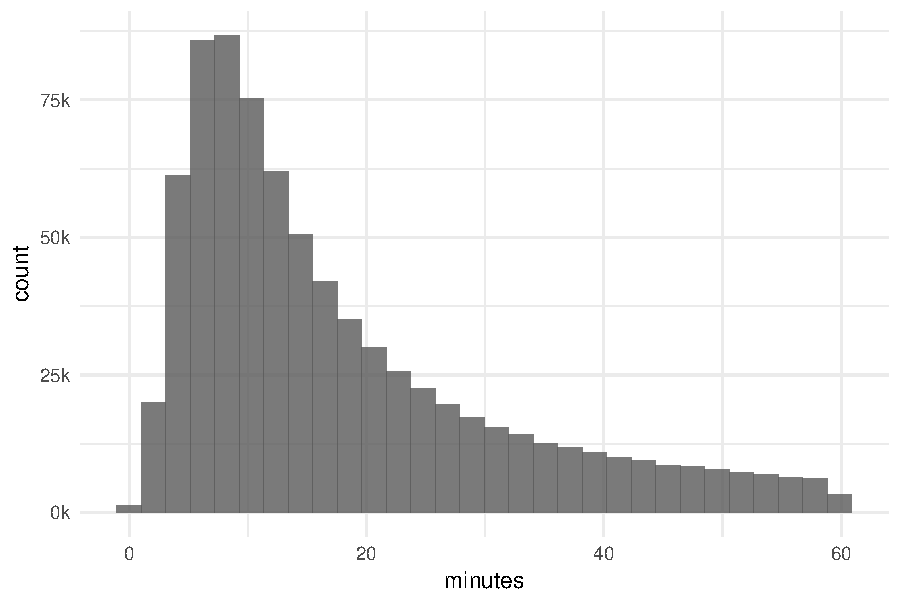
\includegraphics[width=0.8\linewidth]{img/idletime_hist.pdf}
        \subcaption{Distribution of idle time after trip end}
        \label{fig:idlehist}
    \end{minipage}\hfill
    \begin{minipage}[tb]{.8\linewidth}
        \centering
        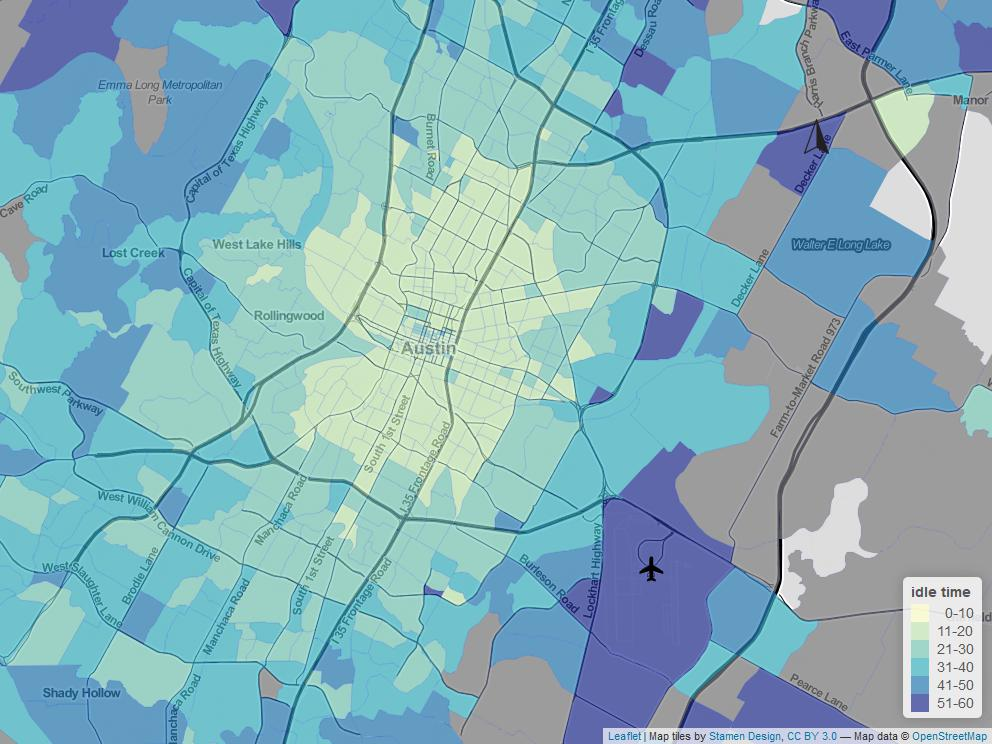
\includegraphics[width=0.8\linewidth]{img/idletime_spatial.jpeg}
        \subcaption{Median idle minutes in between trips by TAZ}
        \label{fig:idlemap}
    \end{minipage}%
    \caption{Histogram of productivity considering all trips}
    \label{fig:idledist}
\end{figure}


\subsection{Construction of the Spatio-Temporal Graph}
\label{section:graph}

The TAZs of Austin are shown in Figure \ref{fig:areatypes}. The advantage of using them over a regular grid discretization is that their size vary accordingly to the traffic intensity, which is also correlated to the number of trips present in the dataset. We thus have a high resolution near downtown and a low resolution in more rural areas. A total of $1,333$ TAZs were considered, requiring that at least one trip originated or ended in that location. Time was discretized hourly, with a periodicity of one week, for a total of $168=24\times7$ time periods.

Altogether, we considered $223,944=168\times1,333$ units of observation, which we used as the vertices of an undirected spatio-temporal graph. Figure \ref{fig:prod_spacetime} shows the total counts of trips aggregating marginally for each time unit and for each space unit. When considered marginally, all space units and all time units have some data. However, once we split by both space and time, only 102,600 of the 223,944 nodes (45.8\%) have some data. 

We construct a set of edges $E$ as the union of a disjoint set of spatial and temporal edges $E=E_S\cup E_T$. The set $E_S$ of edges in the spatial direction was constructed geographically, drawing an edge for all geographically adjacent TAZs for spatial slice at every time. We excluded a few TAZs that were disconnected to the largest connected component of the graph. Edges in the temporal direction $E_T$ were built for every time slice, i.e., joining the vertices for a same TAZ in subsequent hours. An extra edge $(s,168)$ between $(s,1)$ was added for every TAZ $s$ to account for the weekly periodicity. 


\begin{figure}[tb]
    \centering
    \begin{subfigure}[a]{.95\linewidth}
        \centering
        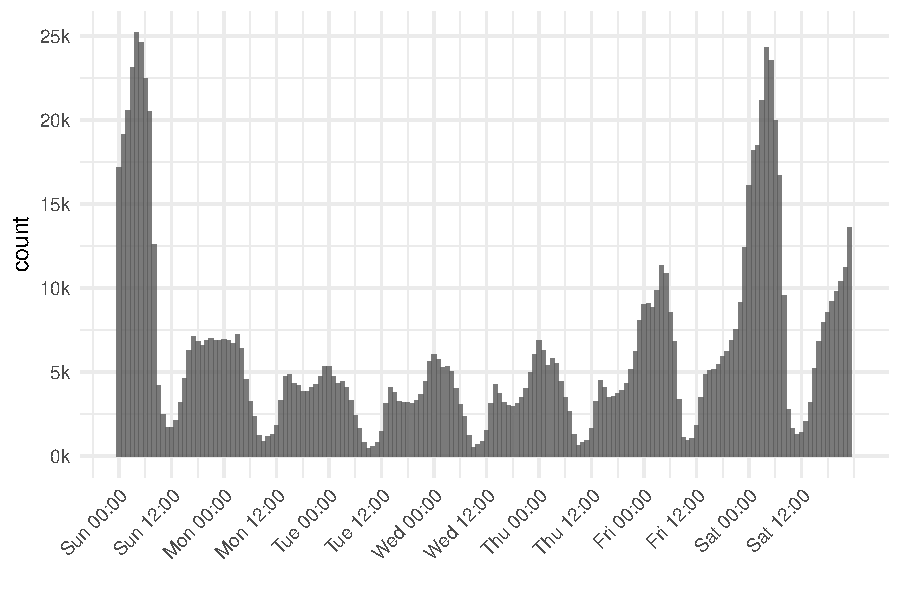
\includegraphics[width=0.7\linewidth]{img/prodhist_timely.pdf}
        \caption{Counts aggregated by time units}
        \label{fig:prod:timely}
    \end{subfigure}%\\
    \hfill
    \begin{subfigure}[b]{.95\linewidth}
        \centering
        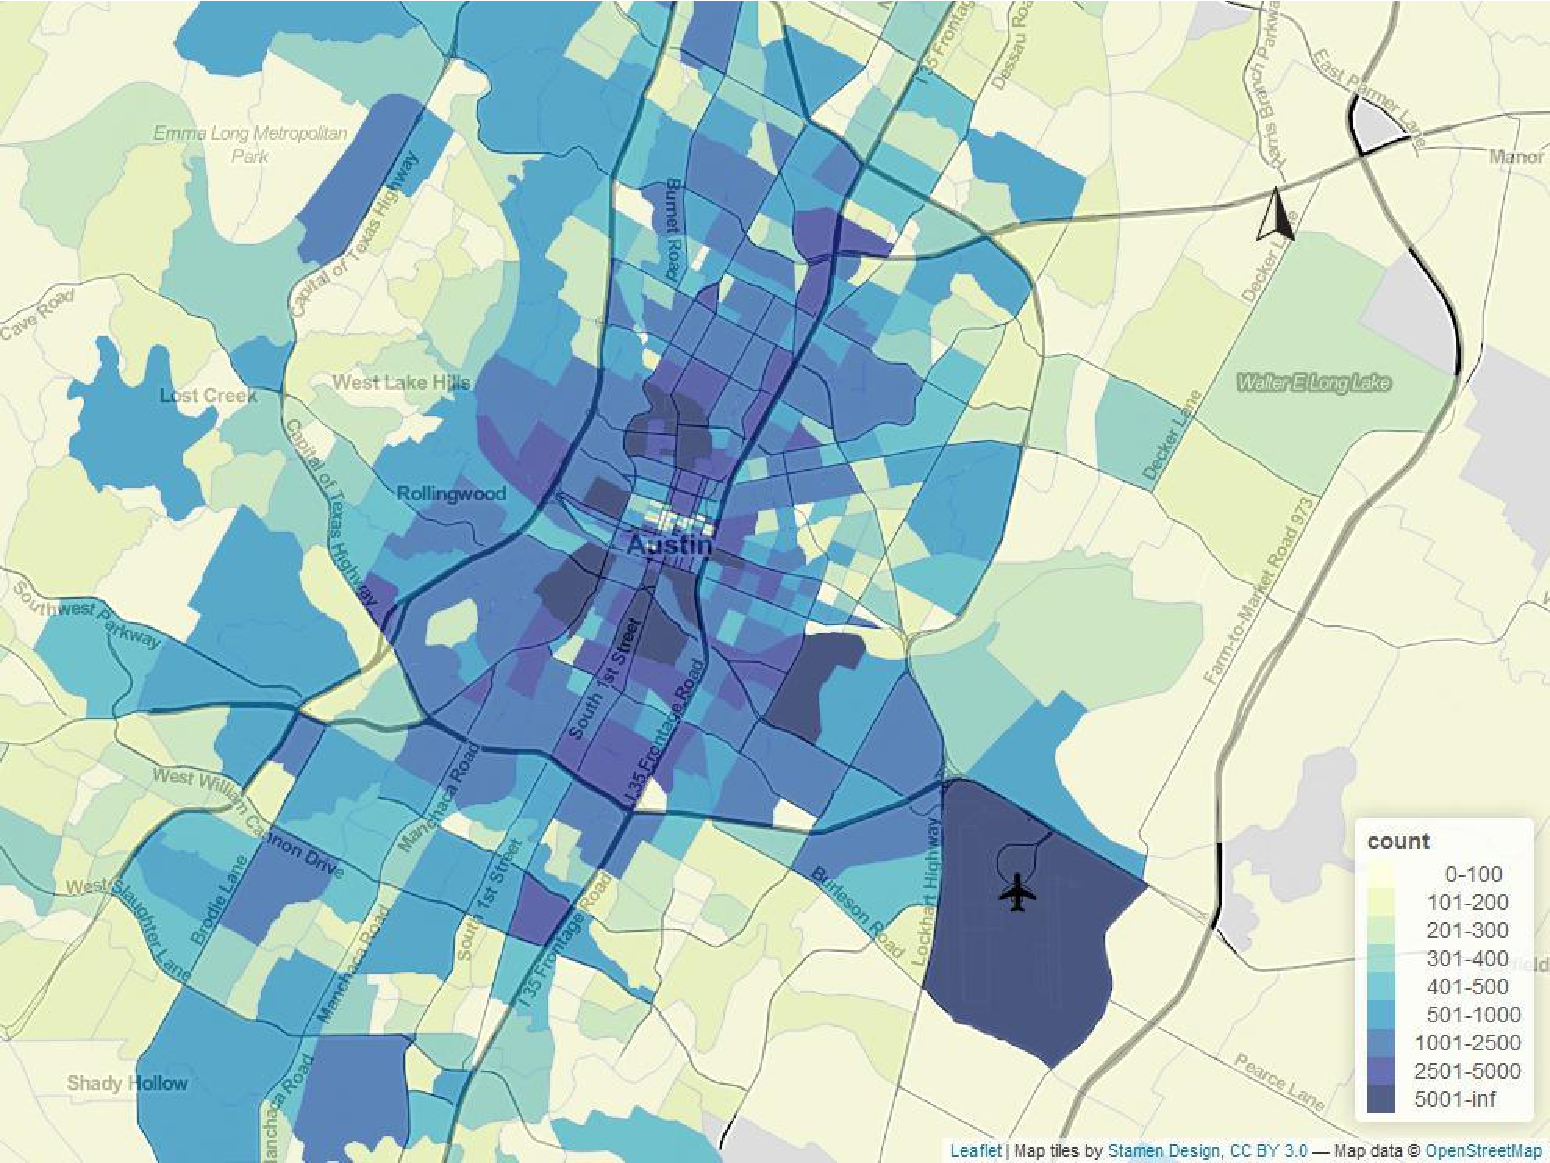
\includegraphics[width=0.7\linewidth]{img/prodhist_spatial.pdf}
        \caption{Counts aggregated by space units}
        \label{fig:prod:spatial}
    \end{subfigure}%
    \caption{Counts of trips marginally aggregated by time and space} 
    \label{fig:prod_spacetime}
\end{figure}

\subsection{Binary Tree Decomposition with Global Quantiles}

We decided to use a binary tree of 5 levels, yielding 32 bins. To choose this bins smartly, we used quantiles of the global productivity distribution to define splitting points in the range (0, 125) which contains 99.98\% of the data\footnote{After examining the data, there are reasons to belief that the top 0.02\% observations come from failures in the data recording system.}. The resulting cutting points are shown in Figure \ref{fig:splits}. While this choice has the undesirable consequence of making our model choice data-dependent, it brings two great benefits:
\begin{itemize}
    \itemsep0em
    \item It naturally uses resolution in regions that had more observations. Alleviating the effects of discretization, and decreasing the need of deeper binary trees.
    \item Unless the local distribution of a vertex dramatically differs from the global distribution, it generates better balanced splits, in the sense that the quantity of observations left and right of each split is more similar; this greatly improved the inference process, since logistic regression does not perform well in highly unbalanced data scenarios.
\end{itemize}

\begin{figure}[tb]
    \centering
    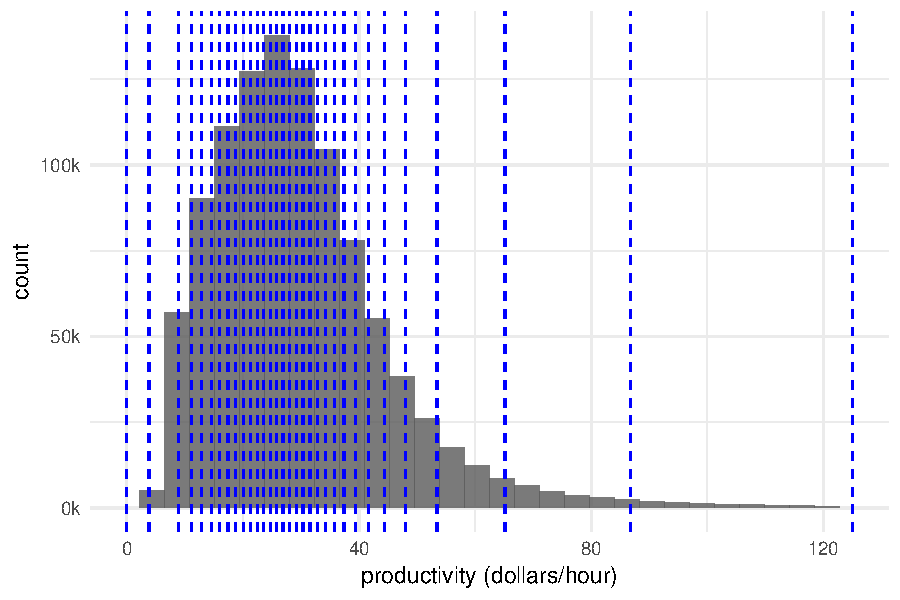
\includegraphics[width=0.55\linewidth]{img/splits.pdf}
    \caption{Vertical dashed lines are the splits used by the binary tree constructed using the quantiles of the global distribution shown in gray.}
    \label{fig:splits}
\end{figure}

\subsection{Hyper-parameter Tuning with Bayesian Optimization}

We used the Bayesian Optimization procedure that we described in section \ref{sec:hyper}. For the Gaussian process, we use the radial kernel $K_{ij}=\exp(-a \lVert \lambda_i - \lambda_j\rVert^2_2)$ with $a=0.5$ and with a small value of $\sigma=10^{-8}$ for the observation uncertainy.

To exploit parallelism, we proceed in generations; in each step, we use the current estimate of the predictive distribution to generate a sample of hyperparameters with small expected loss. We then estimate of the cross-validated loss for each one of them in parallel. After that, we update the Guassian Process and sample a new generation of candidates. In our case, 10 generations of size 16 worked well. 


\subsection{Results}

\subsubsection{Overview of the inference results}

Figure \ref{fig:spacetime-densities} shows the estimated densities. We include five locations that have distinct characteristics that highlight different aspects of the inference. Table \ref{tbl:locations} shows a summary description of the selected sites. We choose central areas with high and low demand (university, downtown, Red River \& 12th), two suburbs with different trip count (Domain and Pflugerville), and the airport area. We show the estimates in intervals of 12 hours during 3am and 3pm. Several interesting qualitative remarks are readily available:

\begin{itemize}
    \item \textit{Not all days are equal}. When considering whether we should include a time observation for each time of the week or just each day, we suspected that each day had slightly different dynamics. We see that in a typical Wednesday 8am, most locations have a density close the global mean, whereas in a typical weekend morning, the locations in the central area (University, downtown, Red River \& 12th) have higher productivity. Mondays and Fridays have also higher productivity than the rest of business days. 
    \item \textit{Smoothing is turned on}. With a few exceptions, the estimates of the locations we chose in central Austin (University, downtown and Red river \& 12th). This is particularly remarkable since Red river had almost no observations. It is also evident regions without observations are not pull towards the global mean, since the region behaves very differently from the global mean.
    \item \textit{We recover periodic patterns}. In our analysis, we chose not to create edges between different days of the week at the same time of the day (e.g., there is no direct edge between a Monday 8pm and Tuesday 8pm). Nevertheless, we do observe periodic patterns for some locations, notably, the airport. Every morning around 8am its distribution is close the global mean, however, every afternoon it is shifted downwards.
\end{itemize}


\begin{table}[tb]
    \centering
    \begin{tabular}{c|p{10cm}}
        \textbf{Location} & \textbf{Description} \\ \hline
        Airport &  Austin-Bergstrom International Airport. It is the single TAZ with more trips. \\ \hline
        The Domain & Office, retail, and residential center outside central Austin. It has medium-low density of trips. \\ \hline
        Pflugerville & Large suburban area located far from the central area. It has low count of trips.  \\ \hline
        University & The University of Texas at Austin main campus. It is located adjacent to central business district. It has a high number of trips.  \\ \hline
        Downtown &  Central business district. It comprises several small TAZs with a large number of trip counts. An arbitrary TAZ was selected in the intersection of 6th \& Guadalupe St. \\ \hline
        Red River \& 12th & Red River is a popular street with restaurants and bars near the central area. However, the exact TAZ that contains the intersection with 12th has a very low trip count.
    \end{tabular}
    \caption{Locations used in figure \ref{fig:spacetime-densities} for comparison of density estimates}
    \label{tbl:locations}
\end{table}

\begin{figure}[tb]
    \centering
    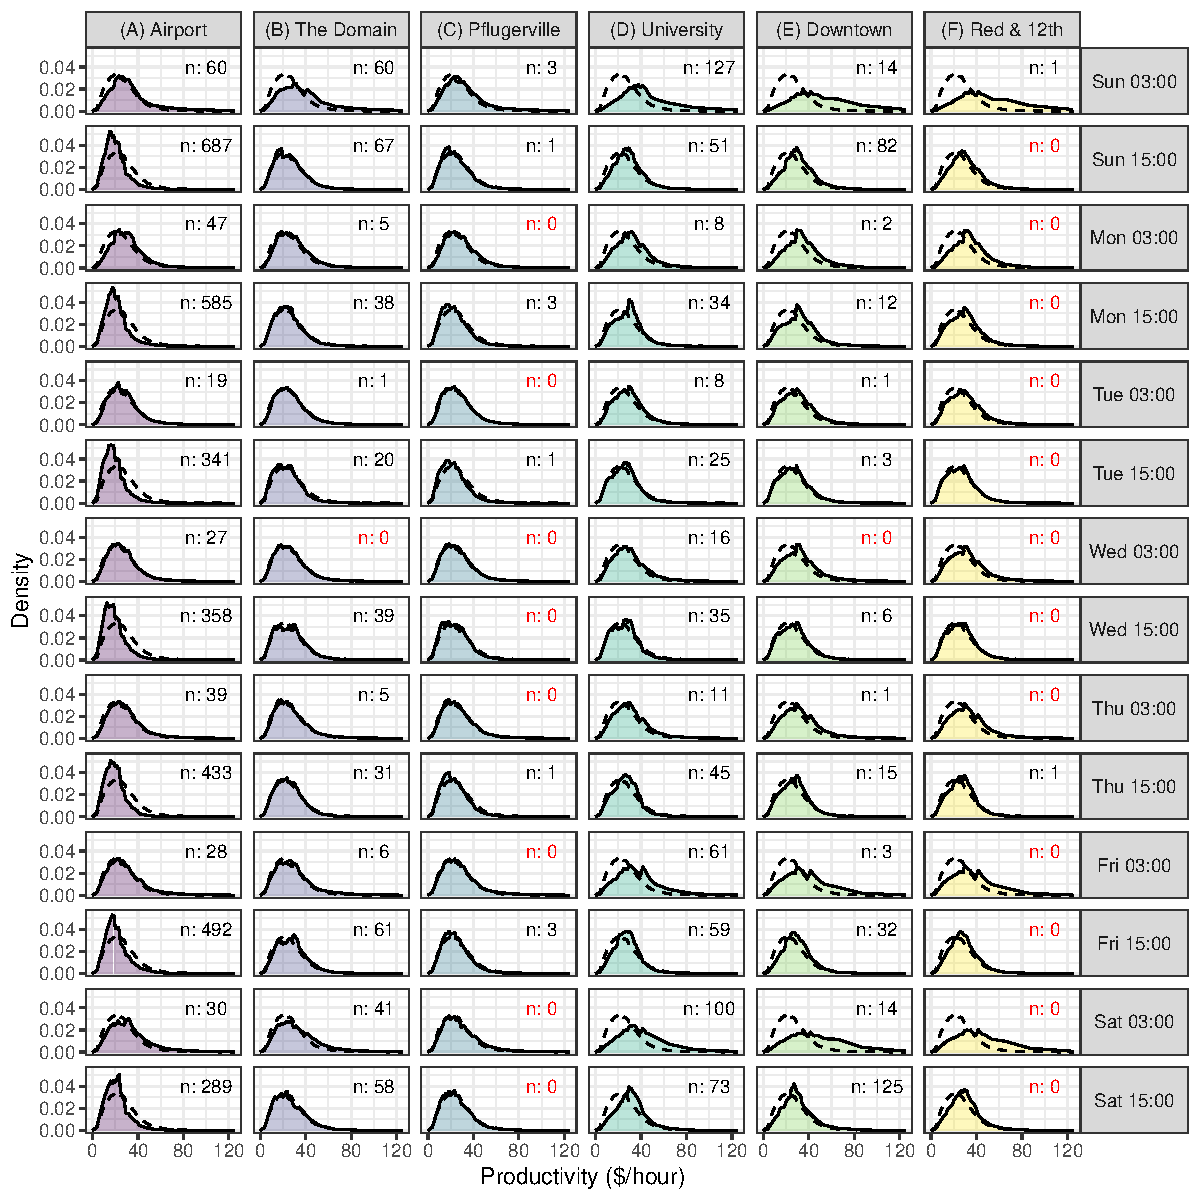
\includegraphics[width=0.98\linewidth]{img/densities_spacetime.pdf}
    \caption{Driver Productivity by Time and Location. The global distribution is shown (dashed); the number of observed data points in the corresponding node of the graph is shown in the upright corner of each density plot (n). Time is shown every 12 hours.}
    \label{fig:spacetime-densities}
\end{figure} 


To further evaluate the time smoothness of the estimates, we show in figure \ref{fig:airport-densities} the estimates at the airport area in intervals of two hours. This completes the picture of the periodic pattern found in figure \ref{fig:spacetime-densities}, since it shows a smooth transition between mornings, when the distribution of productivity is closer to the global mean, to afternoons, when it is smaller. It is interesting to mention that while other locations showed a very different distribution during weekends and business days, the airport is more similar every day.



\begin{figure}[tb]
    \centering
    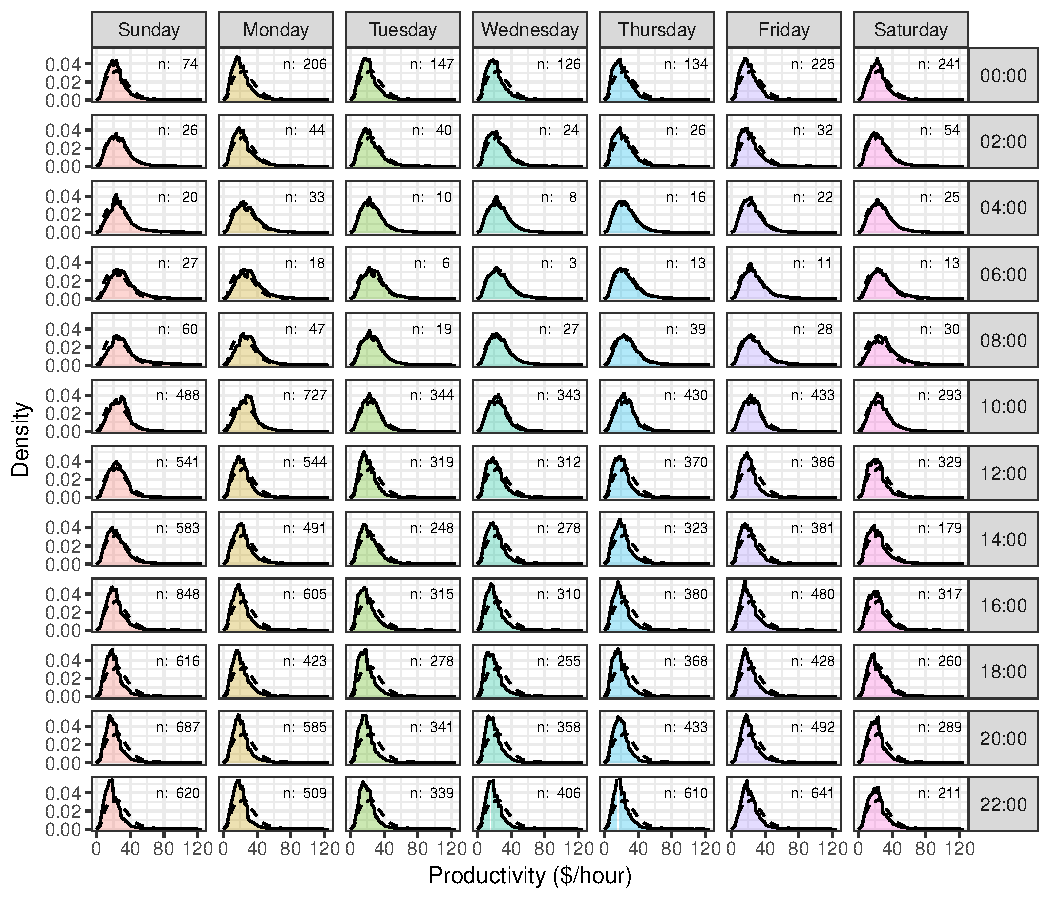
\includegraphics[width=0.98\linewidth]{img/densities_airport.pdf}
    \caption{Driver Productivity of the Airport TAZ. The global distribution (dashed); the number of arriving flights during the observation period (a); the number of departing flights (d); the number of observations in the dataset (n). Time is shown every two hours for the seven days of the week.}
    \label{fig:airport-densities}
\end{figure}


\subsubsection{Investigating driver productivity}

 We present a list of interesting scientific enquiries that can be answered using the full distributions of productivity at each location and time. 
 
 \begin{enumerate}
     \item \textit{Tail probabilities}: What is the probability of not exceeding a specific salary? We compare to standardized living wages in Travis County, TX \citep{nadeau-2017}. 
     \item \textit{Quantiles}: How many dollars per hour constitute the $\alpha$-level quantile? We are interested in assessing the risk of the $\alpha$\% worst performers.
 \end{enumerate}
 
 We provide answers to some of these questions in this section; the others are included in the supplemental material. 

{\bfseries \itshape Tail probabilities: the risk of not attaining a living wage}. We seek to estimate the probability that a driver will obtain a minimum living salary. Table \ref{tbl:livingwages} shows estimated living wages for families living in Austin in 2017 \citep{nadeau-2017}. 

To these wages, we must add the activity-specific additional costs such as the fixed fee of \$0.99 charged per trip charged by RideAustin as well as car maintenance, which on average lies around \$6.40 hourly pretax and \$4.78 hourly after tax deductions \citep{mishel-2018} \citep{hall-etal-2016}. Since a driver completes more than one trip per hour, we rounded up the costs to \$6.00. The final reference values including costs are also presented in table \ref{tbl:livingwages}.

\begin{table}[tb]
    \centering
    \small
    \begin{tabular}{l|l|l|l|l}
        % \hline
        \textbf{\# adults} & 1 adult &  2 adults & 2 adults (1 working) & 1 adult  \\ % \hline
        \textbf{\# children} & 0 children  &   2 children & 2 children & 2 children  \\
       \hline
        \textbf{living wage} & \$12.56  & \$15.64 & \$26.73 & \$28.74  \\ 
        \textbf{living wage+costs} & \$18.56  & \$21.64 & \$32.73 & \$34.74  \\ 
        % \hline
    \end{tabular}
    \caption{Hourly living wages in Austin, TX \citep{nadeau-2017}. The costs are calculated using the \$0.99 RideAustin fee per ride and an estimation of \$4.78 hourly maintenance cost after tax deductions \citep{mishel-2018}.}
    \label{tbl:livingwages}
\end{table}

Figure \ref{fig:wages} shows the results for the case of two working adults with two children (\$21.64) for different times of the week and regions of the city. The remaining cases are included in appendix \ref{appendix:maps_livingwages}. We observe that during a Sunday morning when the traffic is low and there is a high demand (\textit{c.f.} figure \ref{fig:prod:timely}) the probability of exceeding the living wage is close to 90\% near downtown and it decreases to around 70\% as a driver lies farther away from central Austin. In contrast, during at Monday 6pm, with moderate demand but high traffic, the probability ranges from 40\% to 60\%, being worst at the airport. These suggests that drivers are at a high risk of not making a living wage.

\begin{figure}[tb]
    \centering
    \begin{minipage}[tb]{0.48\linewidth}
        \centering
        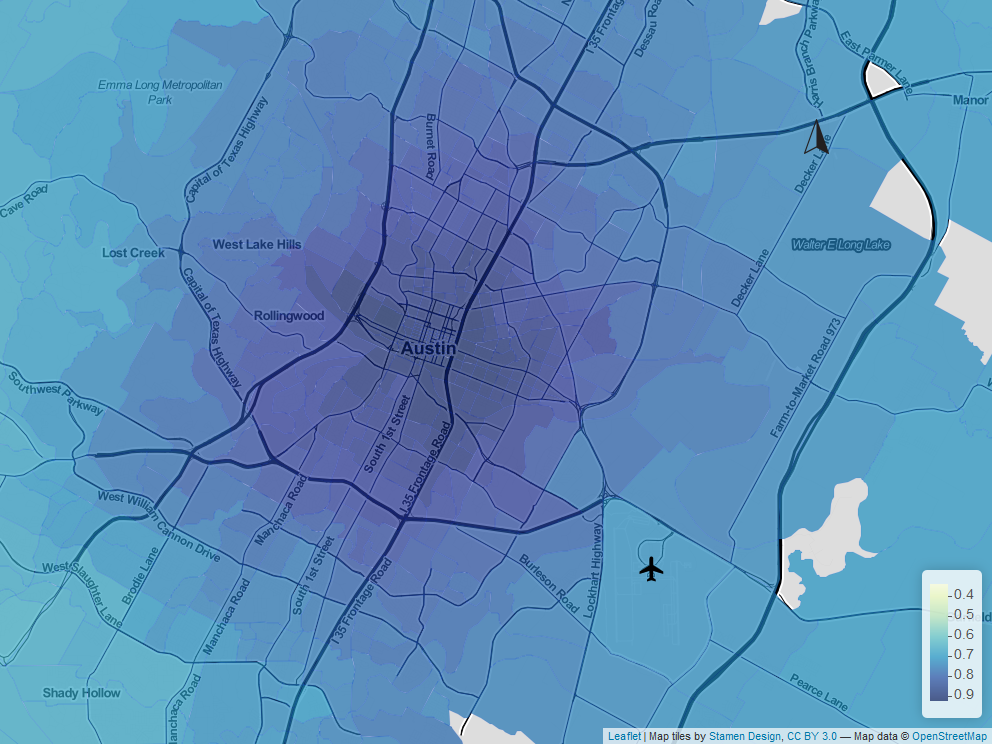
\includegraphics[width=\linewidth]{img/tailprob_21_64__9.png}
        \subcaption{Sunday 3am}
        \label{fig:wages:a}
    \end{minipage}
    \begin{minipage}[tb]{0.48\linewidth}
        \centering
        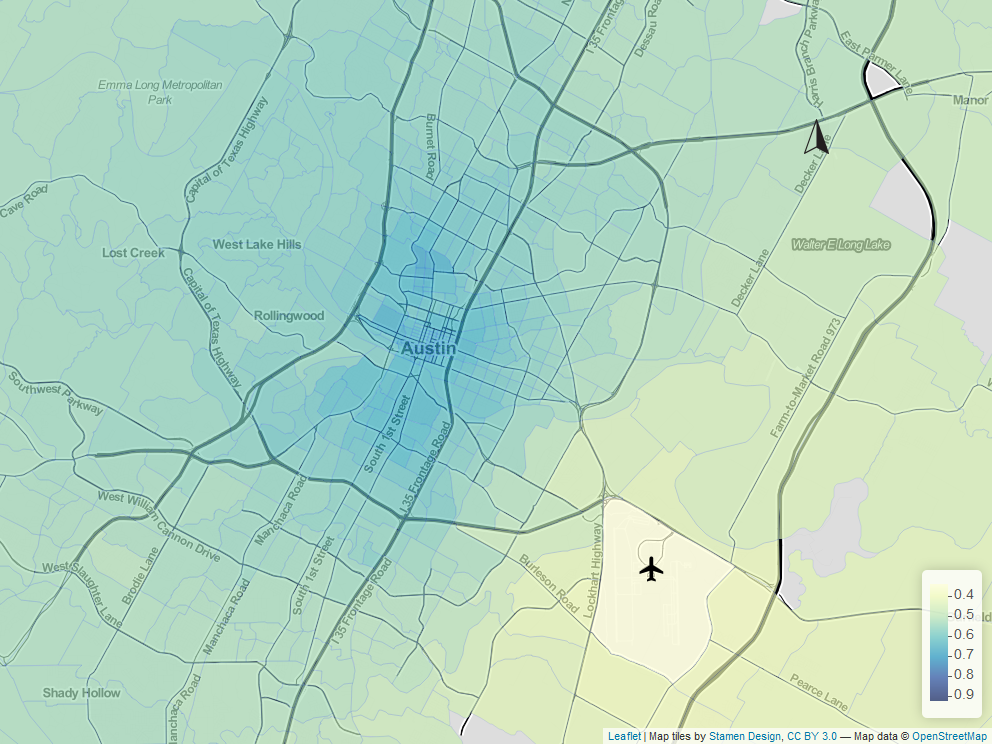
\includegraphics[width=\linewidth]{img/tailprob_21_64__43.png}
        \subcaption{Monday 1pm}
        \label{fig:wages:b}
    \end{minipage}\hfill
    \begin{minipage}[tb]{.48\linewidth}
        \centering
        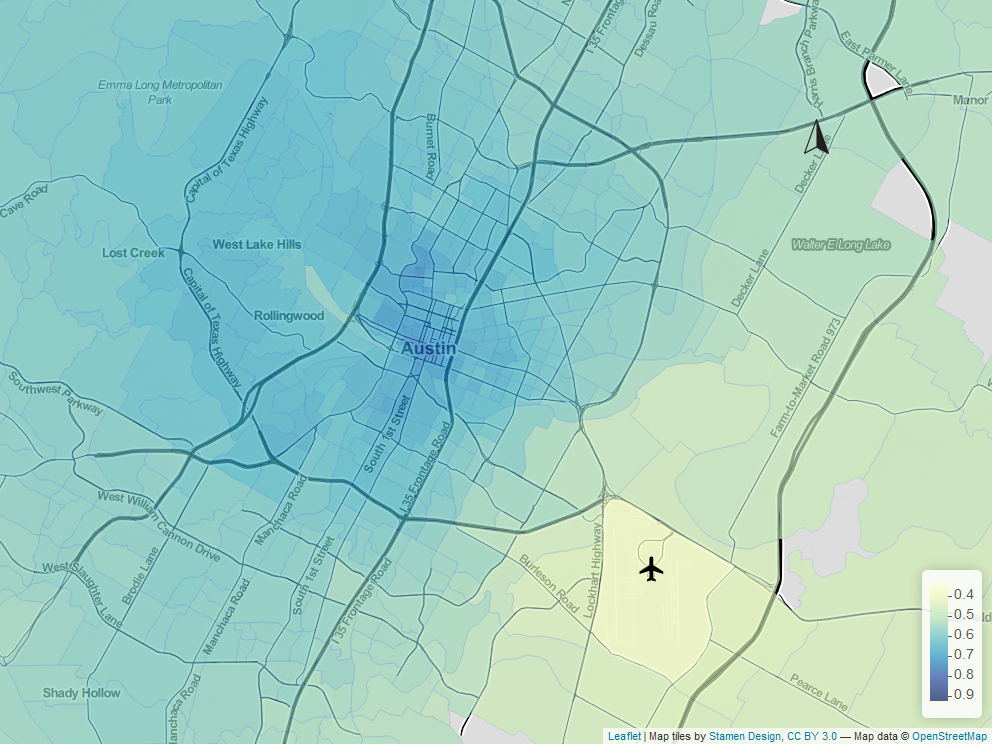
\includegraphics[width=\linewidth]{img/tailprob_21_64__142.png}
        \subcaption{Friday 4pm}
        \label{fig:wages:c}
    \end{minipage}
    \begin{minipage}[tb]{0.48\linewidth}
        \centering
        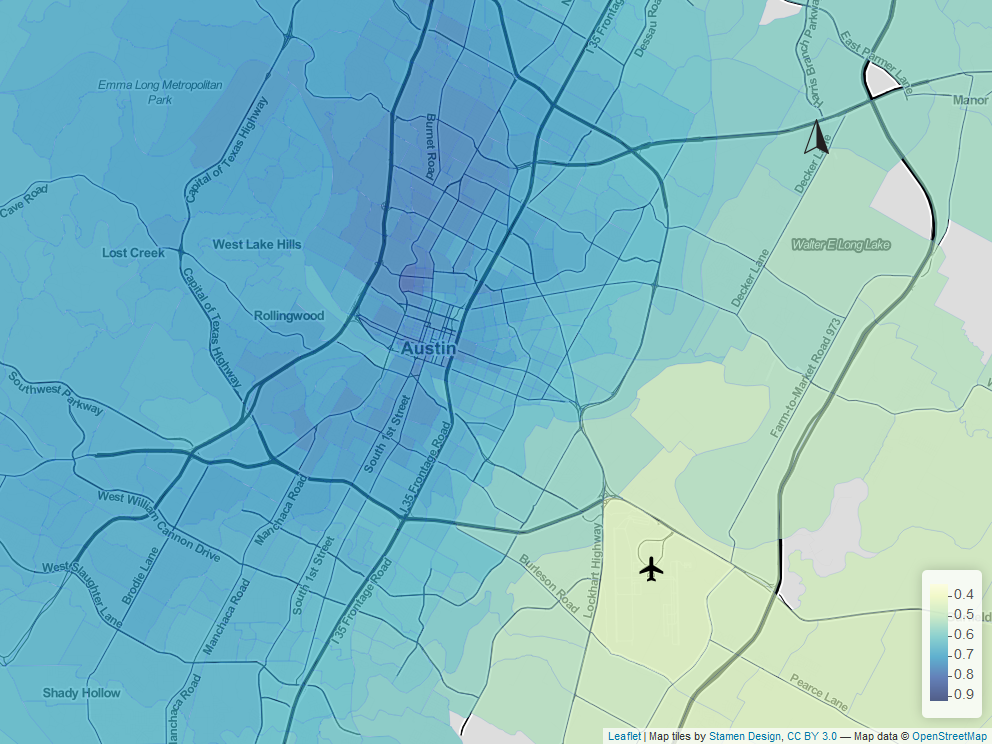
\includegraphics[width=\linewidth]{img/tailprob_21_64__168.png}
        \subcaption{Saturday 6pm}
        \label{fig:wages:d}
    \end{minipage}
    \caption{Probability of exceeding \$21.64 in the next hour given a current location (living wage with costs for two working adults with two children).}
    \label{fig:wages}
\end{figure}

{\bfseries\itshape Quantiles: How bad are the worst performers doing?}. As a company seeking to guarantee the well-being of its workers, it makes sense to target the population at specific levels of risk. One may ask, What is the expected income of the lowest $100 \alpha\%$ percent? That is, for each location and time, we seek to find the quantity
$$
q_\alpha := \min_{q\in[0,125]}P(\mathtt{productivity} > q) > \alpha
$$
Usual interesting values for $\alpha$ are $\{0.1, 0.25, 0.5, 0.75, 0.9\}$. The case $\alpha = 0.1$ is shown in figure \ref{fig:quantiles:0.1}, the rest are included in appendix \ref{appendix:quantiles}. We can see that in a typical Monday 6pm, the rush hour, the lowest $10\%$ quantile is around $\$12$ to $\$15$, being as low as $\$10$ in the airport area. This result should be contrasted with table \ref{tbl:livingwages}, which states that a living wage of a single working adult with no children is above $\$18$. The highest value is attained around the central part of the city during weekend mornings when there is low traffic and high demand (\textit{c.f.} figure \ref{fig:prod:timely}).

\begin{figure}[tb]
    \centering
    \begin{minipage}[tb]{0.48\linewidth}
        \centering
        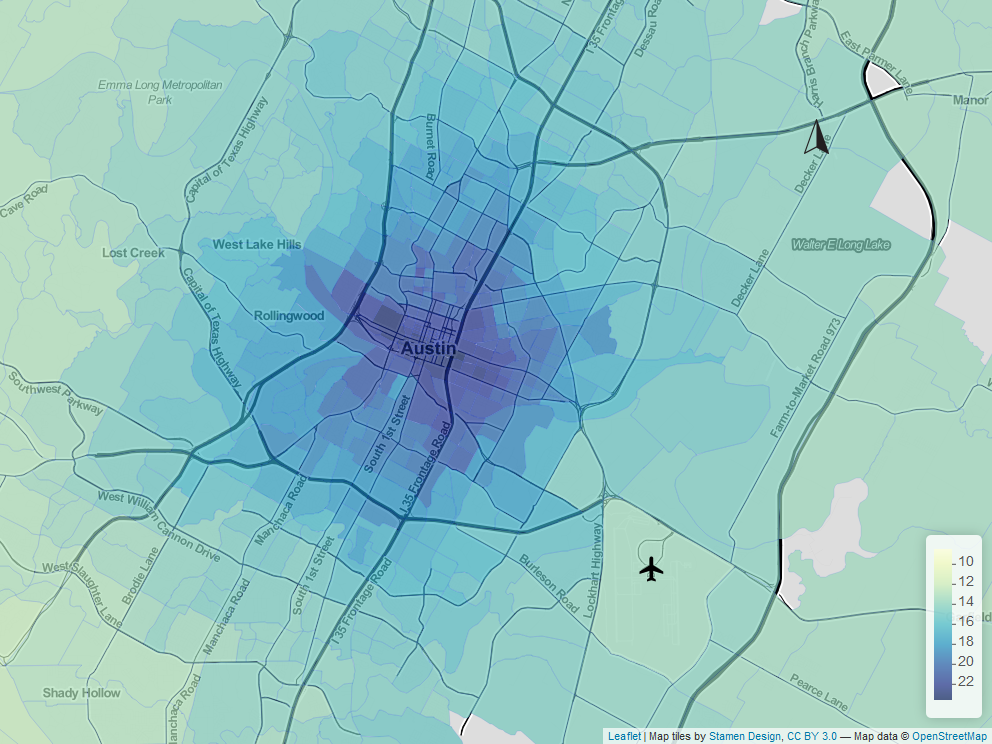
\includegraphics[width=\linewidth]{img/quantile_9_1.png}
        \subcaption{Sunday 3am}
        \label{fig:quantiles:0.1:a}
    \end{minipage}
    \begin{minipage}[tb]{0.48\linewidth}
        \centering
        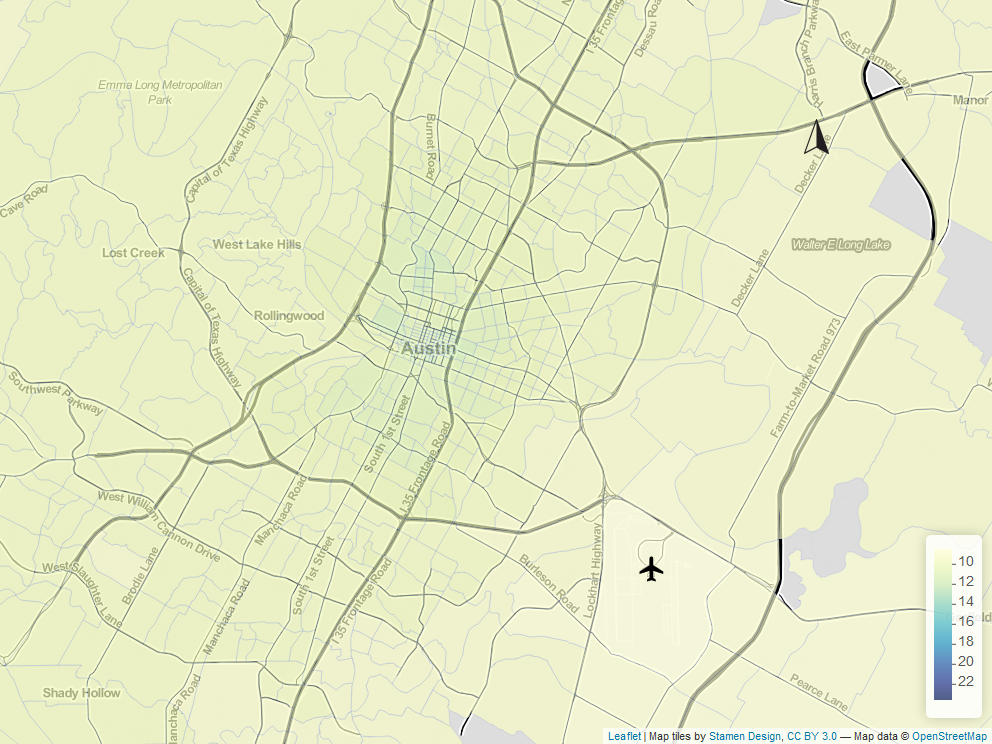
\includegraphics[width=\linewidth]{img/quantile_43_1.png}
        \subcaption{Monday 1pm}
        \label{fig:quantiles:0.1:b}
    \end{minipage}\hfill
    \begin{minipage}[tb]{.48\linewidth}
        \centering
        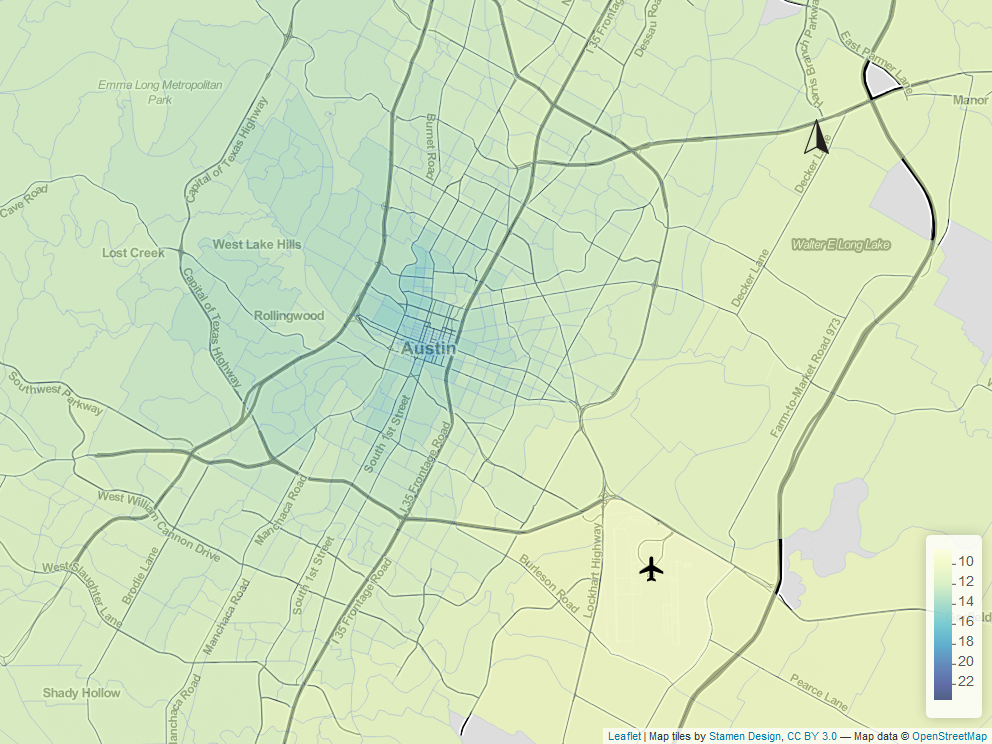
\includegraphics[width=\linewidth]{img/quantile_142_1.png}
        \subcaption{Friday 4pm}
        \label{fig:quantiles:0.1:c}
    \end{minipage}
    \begin{minipage}[tb]{0.48\linewidth}
        \centering
        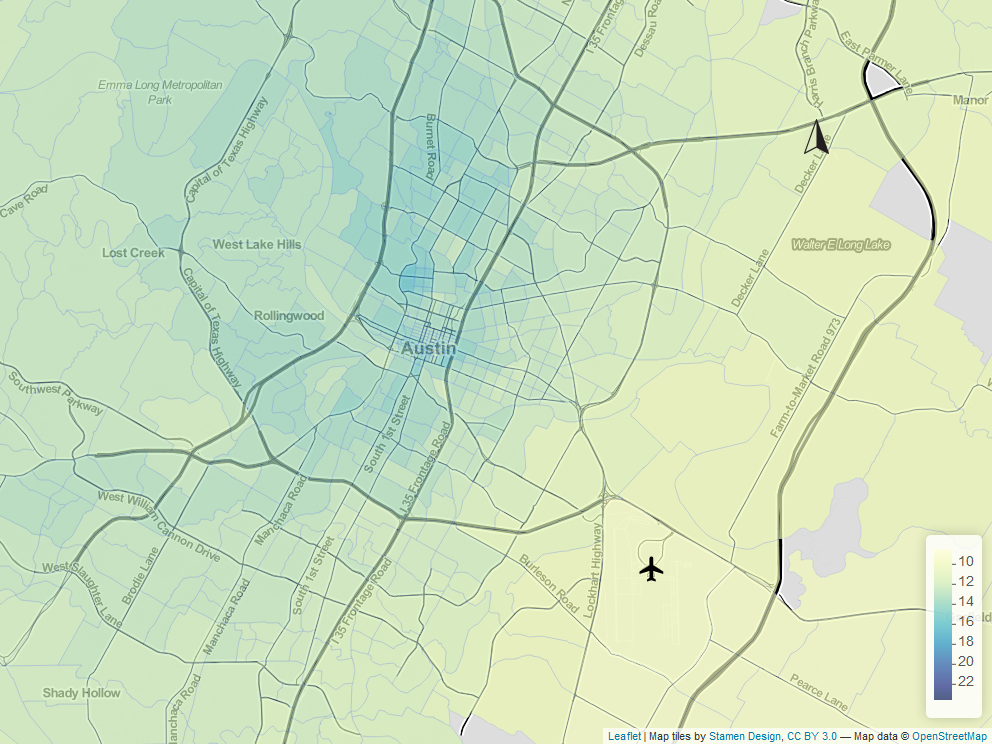
\includegraphics[width=\linewidth]{img/quantile_168_1.png}
        \subcaption{Saturday 6pm}
        \label{fig:quantiles:0.1:d}
    \end{minipage}
    \caption{Lower 10\% quantile of productivity for different times and locations.}
    \label{fig:quantiles:0.1}
\end{figure}

Given that we have quantiles, a natural measure of spread to consider is the inter-quartile range
$$
\text{IQR} = q_{0.75} - q_{0.25}.
$$
This quantity is preferred over standard deviation for skewed distributions such as our measure of productivity. Figure \ref{fig:iqr} shows the IQR for different times and locations. It must be pointed out that this is measure of spread does not take into account the uncertainty arising from the estimation procedure, but only the variability in the estimated densities. Figure \ref{fig:iqr} complements our previous inquiry using tail probabilities and quantiles in the sense that it shows that the highest reward observed Sunday 3am when there's high demand and low traffic, comes accompanied by higher variability, and not only a shift in location.

\begin{figure}[tb]
    \centering
    \begin{minipage}[tb]{0.48\linewidth}
        \centering
        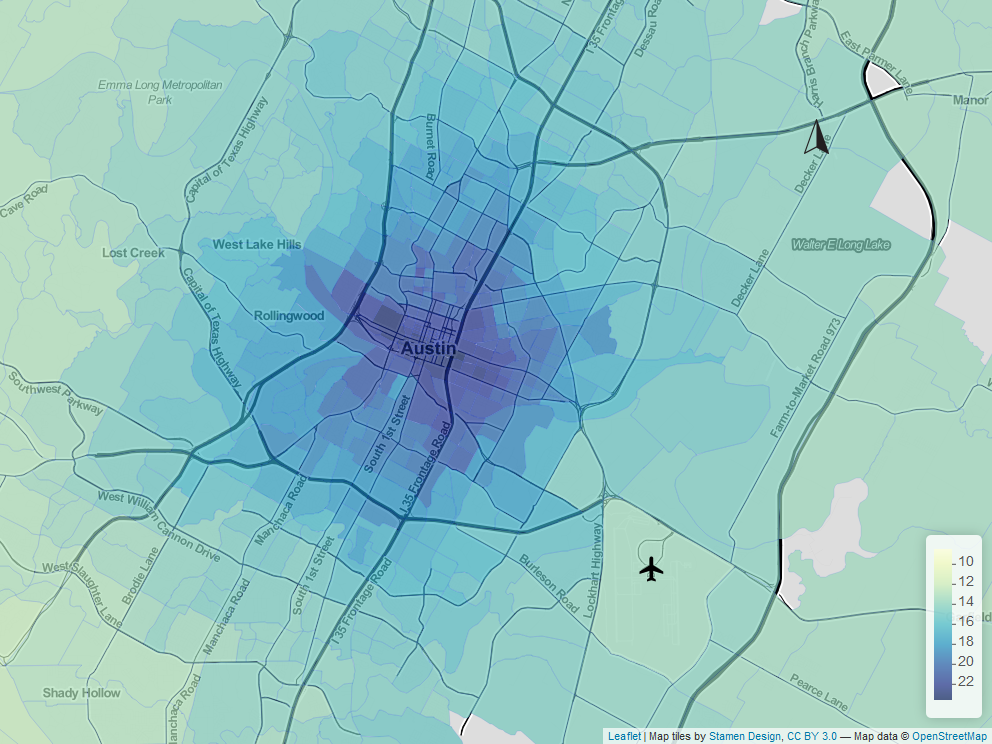
\includegraphics[width=\linewidth]{img/quantile_9_1.png}
        \subcaption{Sunday 3am}
        \label{fig:iqr:a}
    \end{minipage}
    \begin{minipage}[tb]{0.48\linewidth}
        \centering
        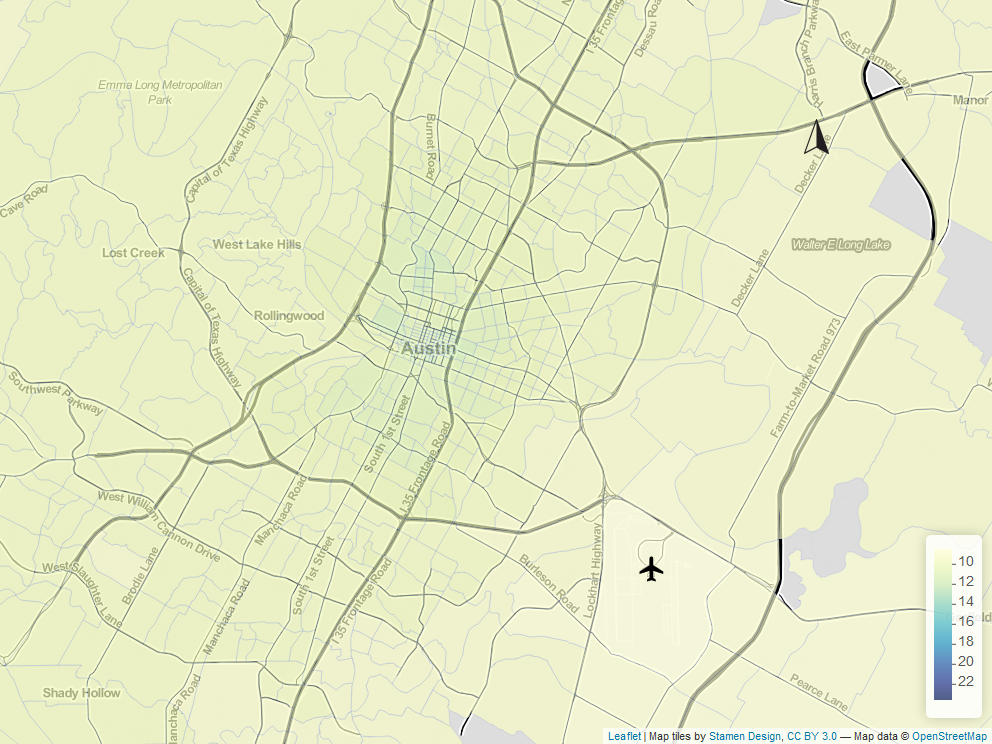
\includegraphics[width=\linewidth]{img/quantile_43_1.png}
        \subcaption{Monday 1pm}
        \label{fig:iqr:b}
    \end{minipage}\hfill
    \begin{minipage}[tb]{.48\linewidth}
        \centering
        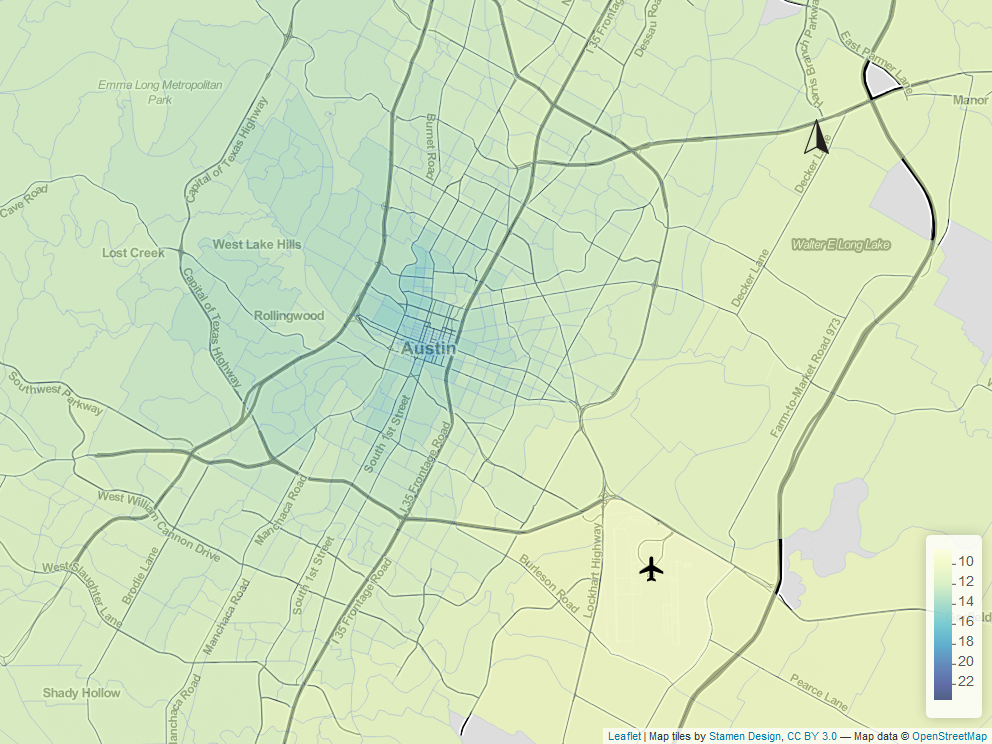
\includegraphics[width=\linewidth]{img/quantile_142_1.png}
        \subcaption{Friday 4pm}
        \label{fig:iqr:c}
    \end{minipage}
    \begin{minipage}[tb]{0.48\linewidth}
        \centering
        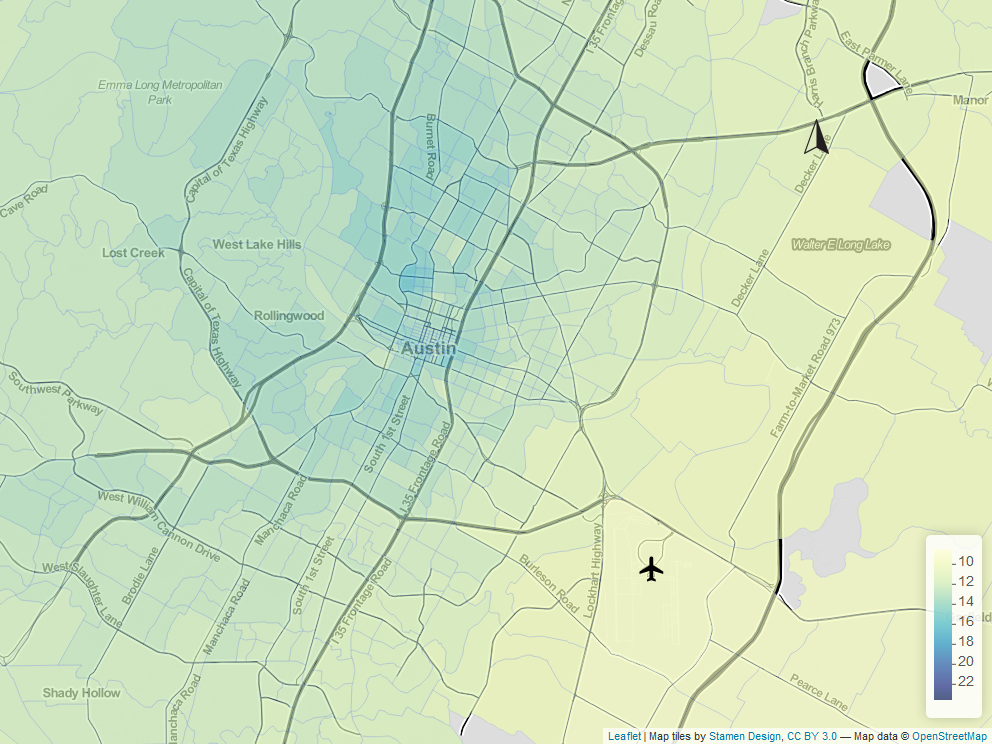
\includegraphics[width=\linewidth]{img/quantile_168_1.png}
        \subcaption{Saturday 6pm}
        \label{fig:iqr:d}
    \end{minipage}
    \caption{IQR of productivity for different times and locations.}
    \label{fig:iqr}
\end{figure}


\section{Concluding remarks}
\label{sec:conc}


\appendix
% \section{Tail probabilities of not exceeding living wage}
\label{appendix:maps_livingwages}

\begin{figure}[htb]
    \centering
    \begin{minipage}[t]{0.48\linewidth}
        \centering
        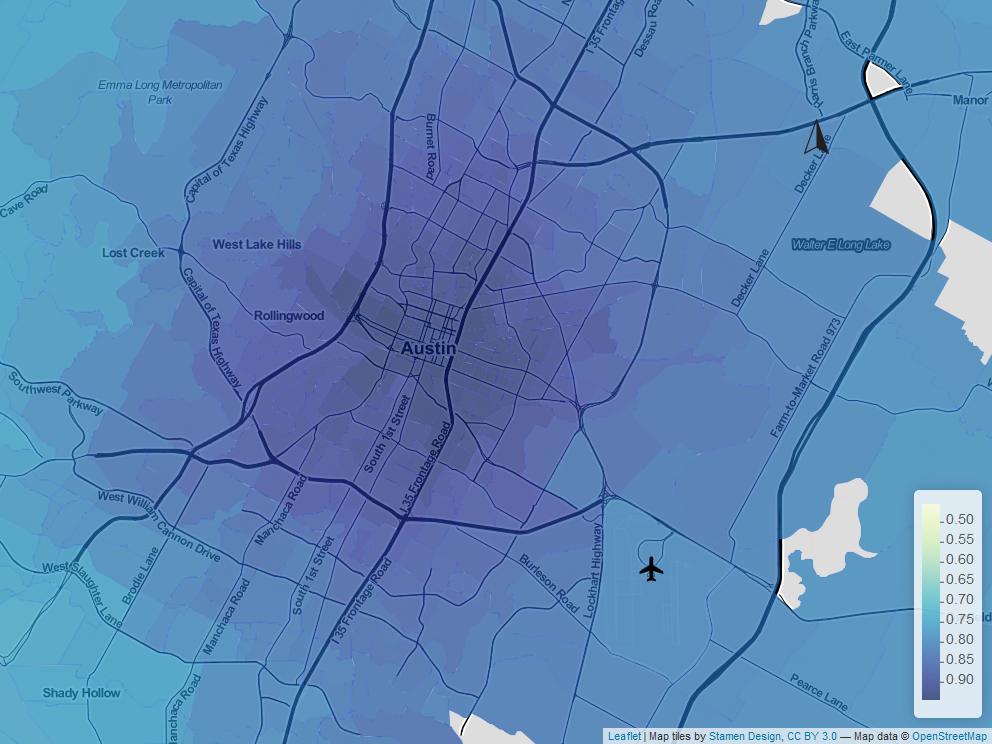
\includegraphics[width=\linewidth]{img/tailprob_18_56__9.png}
        \subcaption{Sunday 8am (weekend low traffic)}
        \label{fig:wages:appendix1:a}
    \end{minipage}
    \begin{minipage}[t]{0.48\linewidth}
        \centering
        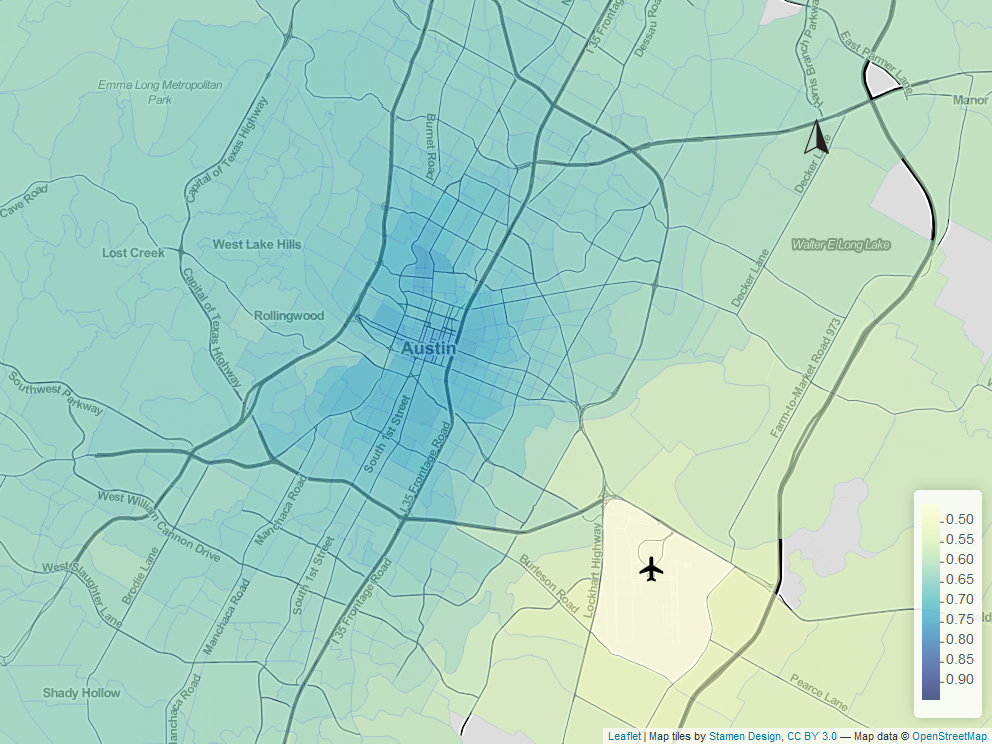
\includegraphics[width=\linewidth]{img/tailprob_18_56__43.png}
        \subcaption{Monday 6pm (weekday rush hour)}
        \label{fig:wages:appendix1:b}
    \end{minipage}\hfill
    \begin{minipage}[t]{.48\linewidth}
        \centering
        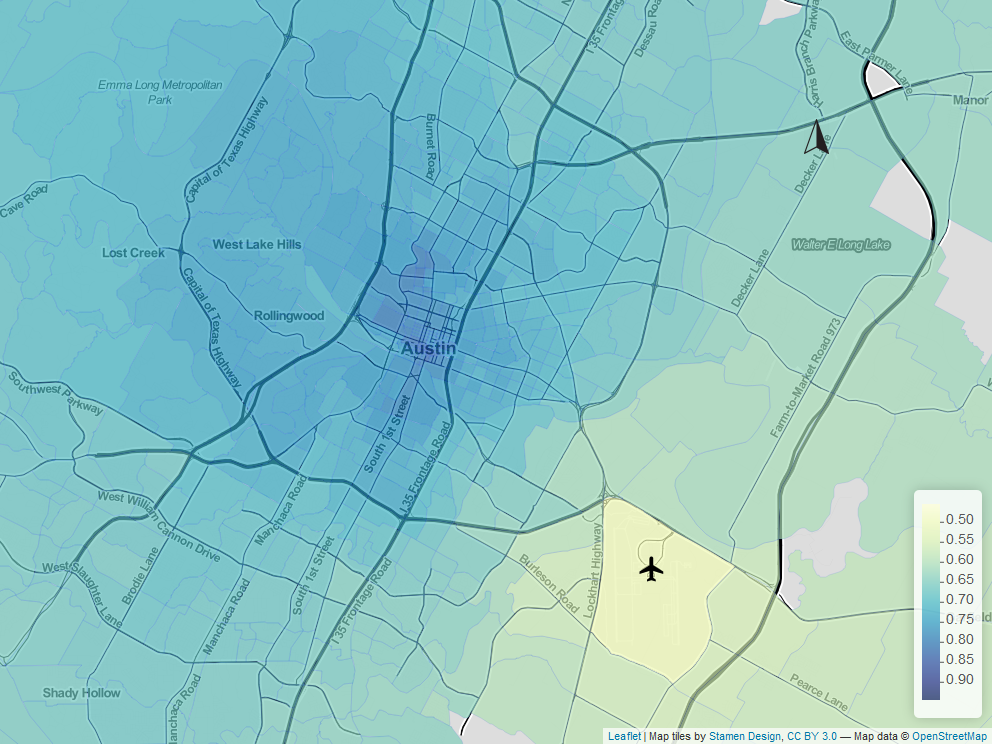
\includegraphics[width=\linewidth]{img/tailprob_18_56__142.png}
        \subcaption{Friday 9pm (weekday social mild traffic)}
        \label{fig:wages:appendix1:c}
    \end{minipage}
    \begin{minipage}[t]{0.48\linewidth}
        \centering
        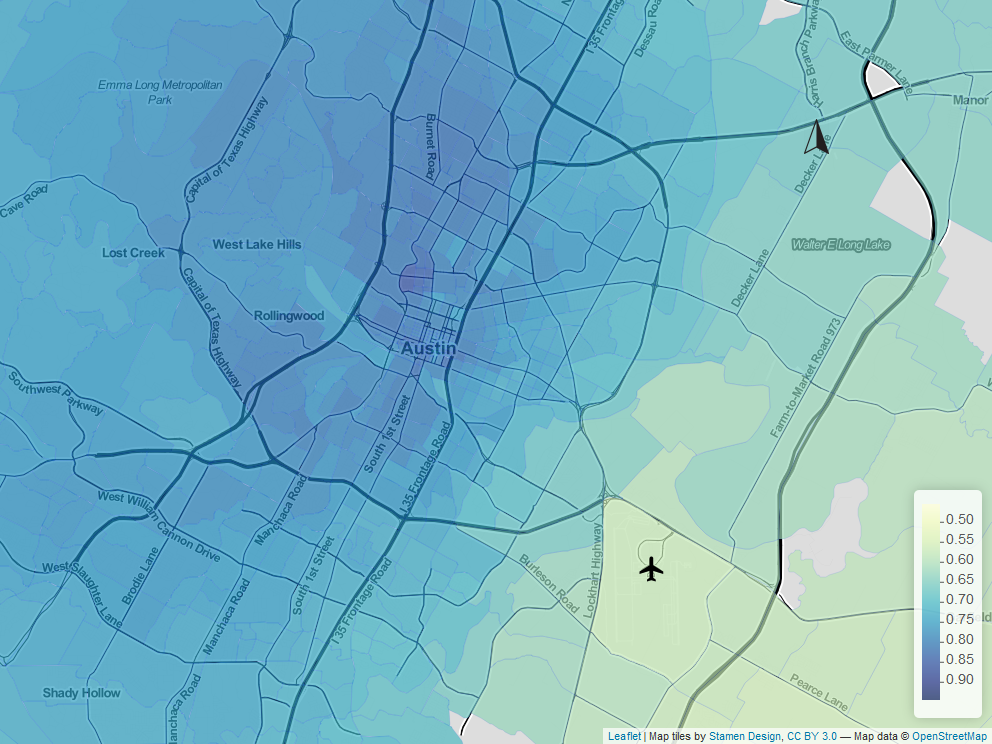
\includegraphics[width=\linewidth]{img/tailprob_18_56__168.png}
        \subcaption{Saturday 11pm (weekend social low traffic)}
        \label{fig:wages:appendix1:d}
    \end{minipage}
    \caption{Probability of exceeding \$18.56 in the next hour given a current location (living wage with costs for one single working adult with no children).}
    \label{fig:wages:appendix1}
\end{figure}


\begin{figure}[htb]
    \centering
    \begin{minipage}[t]{0.48\linewidth}
        \centering
        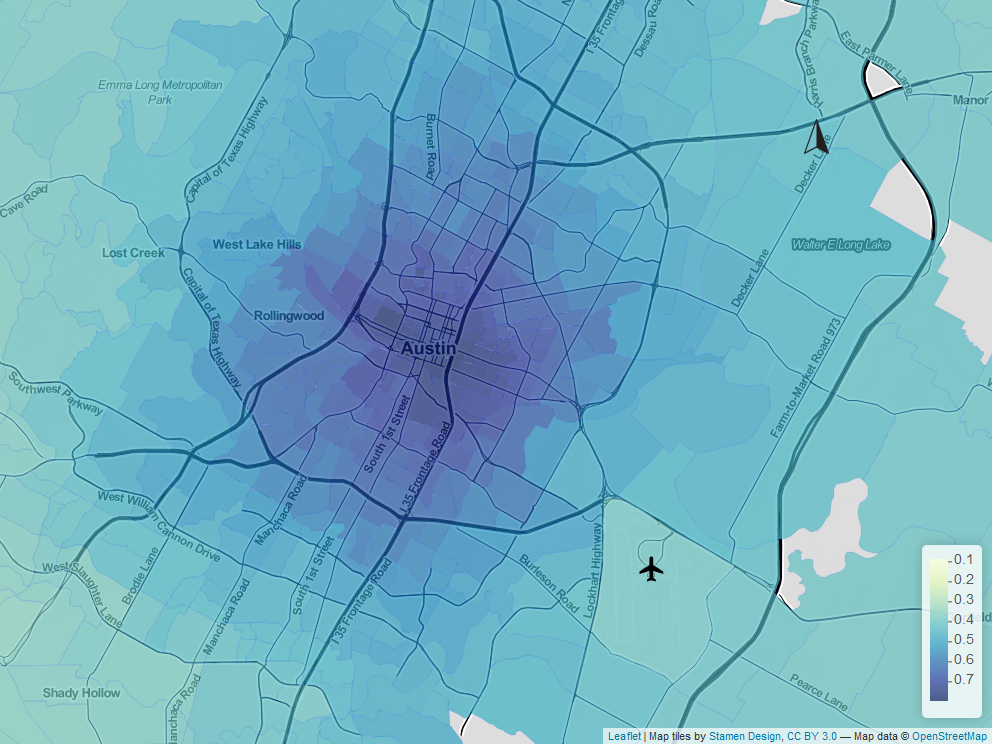
\includegraphics[width=\linewidth]{img/tailprob_32_73__9.png}
        \subcaption{Sunday 8am (weekend low traffic)}
        \label{fig:wages:appendix2:a}
    \end{minipage}
    \begin{minipage}[t]{0.48\linewidth}
        \centering
        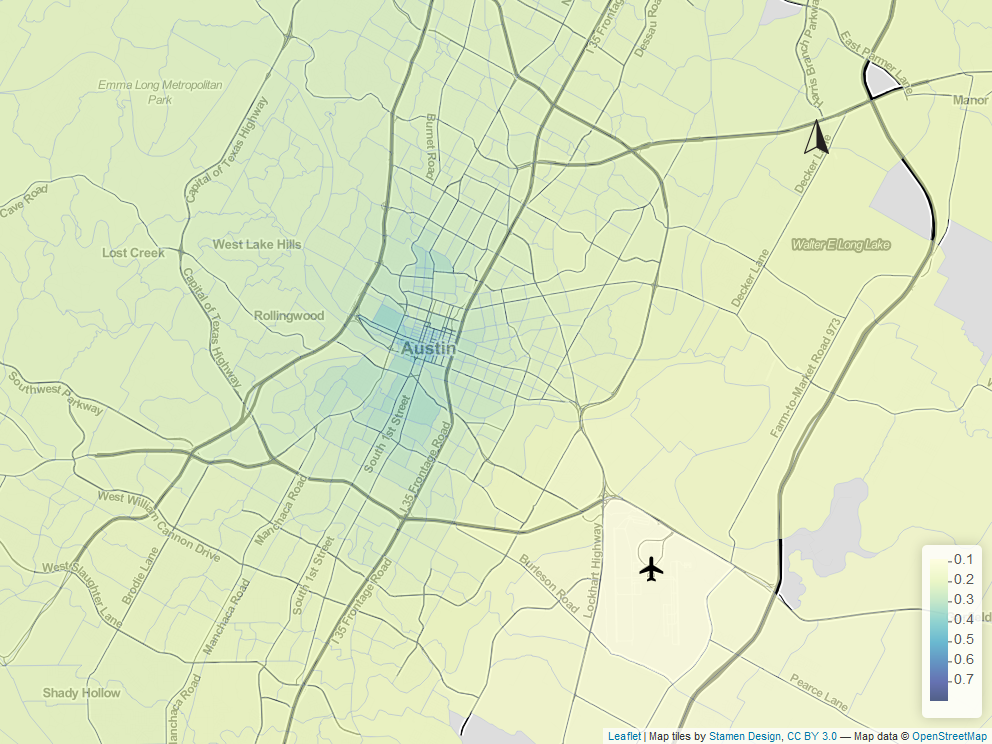
\includegraphics[width=\linewidth]{img/tailprob_32_73__43.png}
        \subcaption{Monday 6pm (weekday rush hour)}
        \label{fig:wages:appendix2:b}
    \end{minipage}\hfill
    \begin{minipage}[t]{.48\linewidth}
        \centering
        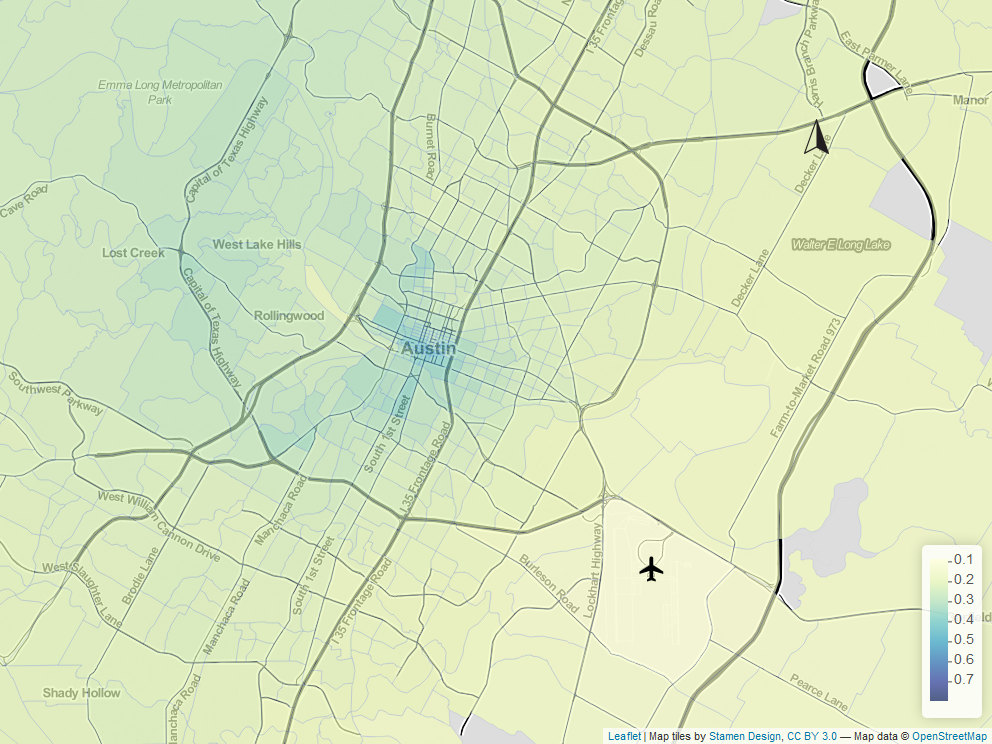
\includegraphics[width=\linewidth]{img/tailprob_32_73__142.png}
        \subcaption{Friday 9pm (weekday social mild traffic)}
        \label{fig:wages:appendix2:c}
    \end{minipage}
    \begin{minipage}[t]{0.48\linewidth}
        \centering
        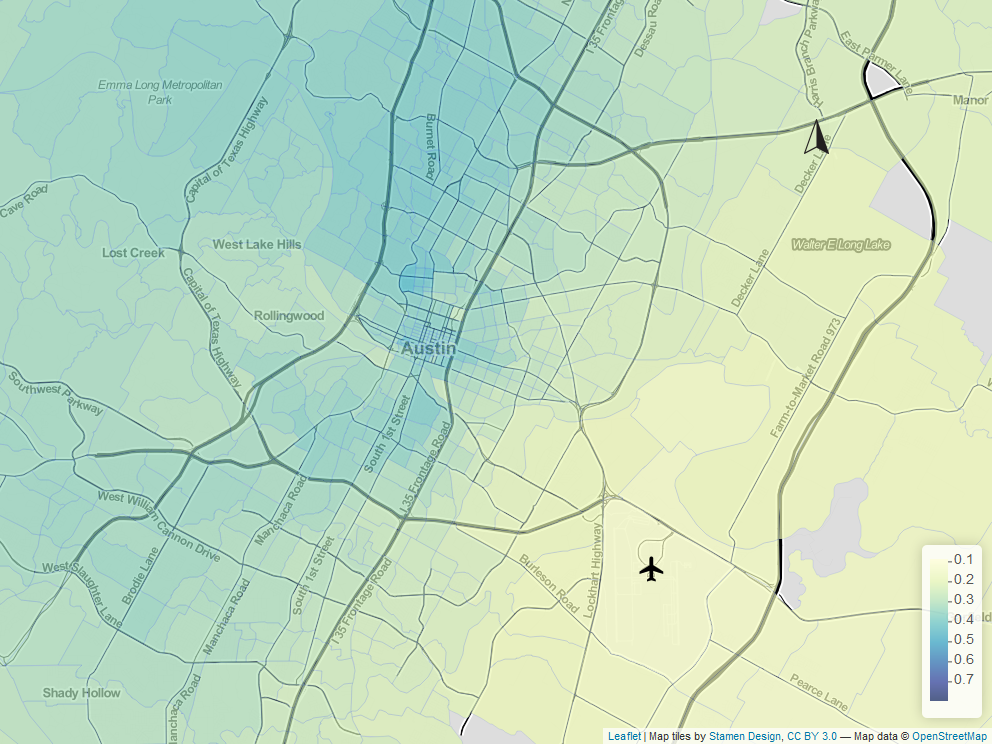
\includegraphics[width=\linewidth]{img/tailprob_32_73__168.png}
        \subcaption{Saturday 11pm (weekend social low traffic)}
        \label{fig:wages:appendix2:d}
    \end{minipage}
    \caption{Probability of exceeding \$32.73 in the next hour given a current location (living wage with costs for two adults, one working, and two children).}
    \label{fig:wages:appendix2}
\end{figure}


\begin{figure}[htb]
    \centering
    \begin{minipage}[t]{0.48\linewidth}
        \centering
        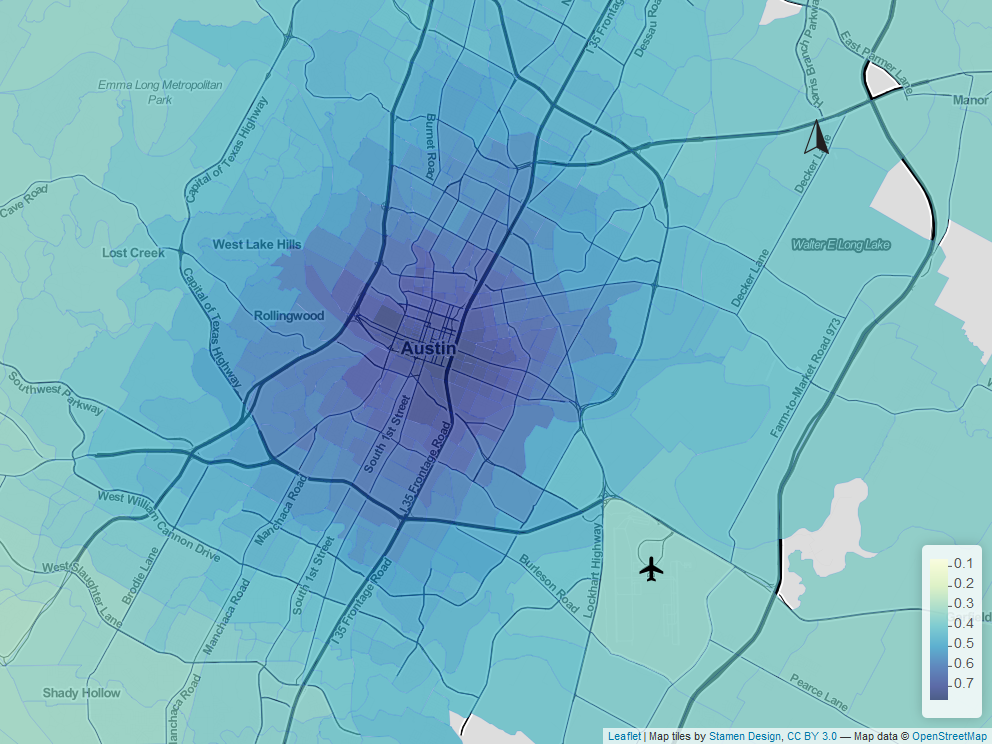
\includegraphics[width=\linewidth]{img/tailprob_34_74__9.png}
        \subcaption{Sunday 8am (weekend low traffic)}
        \label{fig:wages:appendix3:a}
    \end{minipage}
    \begin{minipage}[t]{0.48\linewidth}
        \centering
        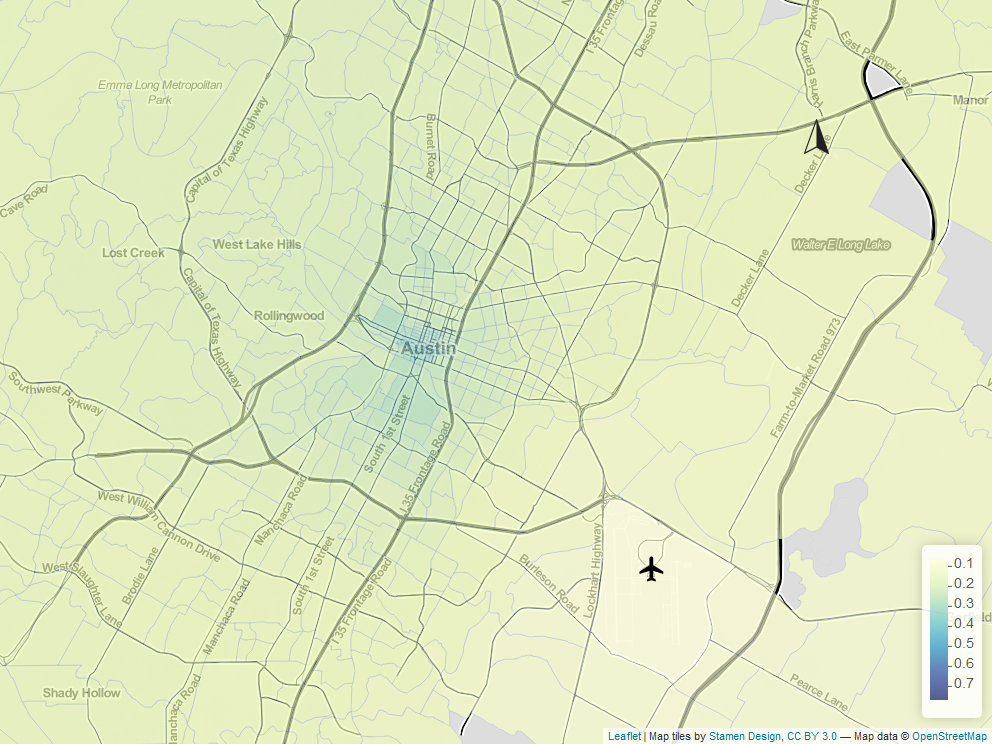
\includegraphics[width=\linewidth]{img/tailprob_34_74__43.png}
        \subcaption{Monday 6pm (weekday rush hour)}
        \label{fig:wages:appendix3:b}
    \end{minipage}\hfill
    \begin{minipage}[t]{.48\linewidth}
        \centering
        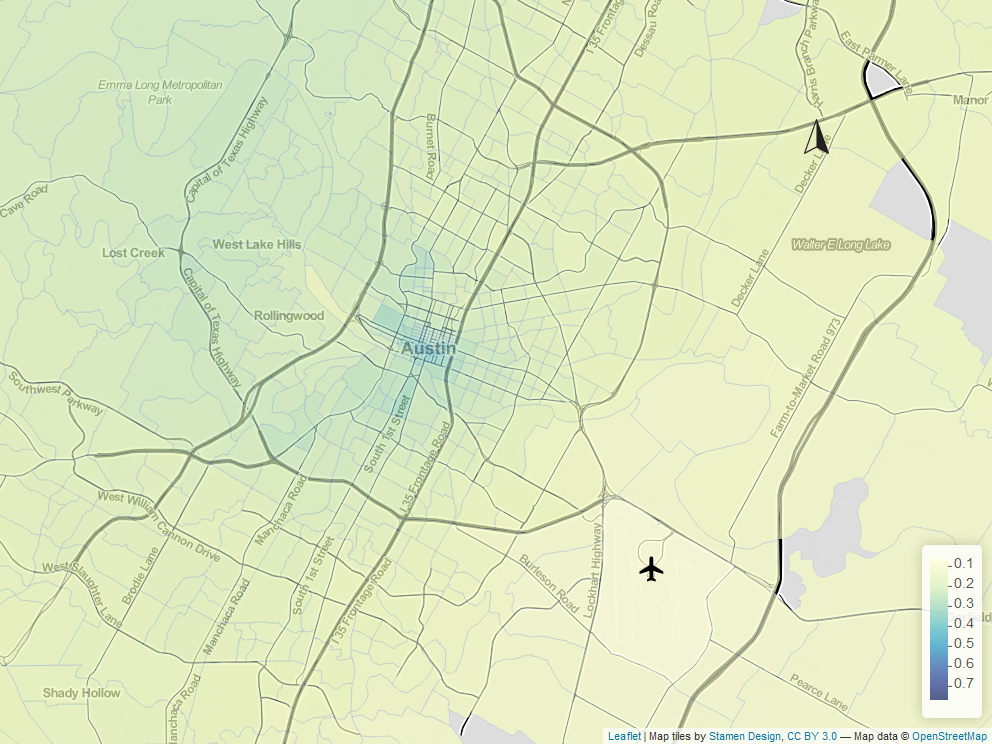
\includegraphics[width=\linewidth]{img/tailprob_34_74__142.png}
        \subcaption{Friday 9pm (weekday social mild traffic)}
        \label{fig:wages:appendix3:c}
    \end{minipage}
    \begin{minipage}[t]{0.48\linewidth}
        \centering
        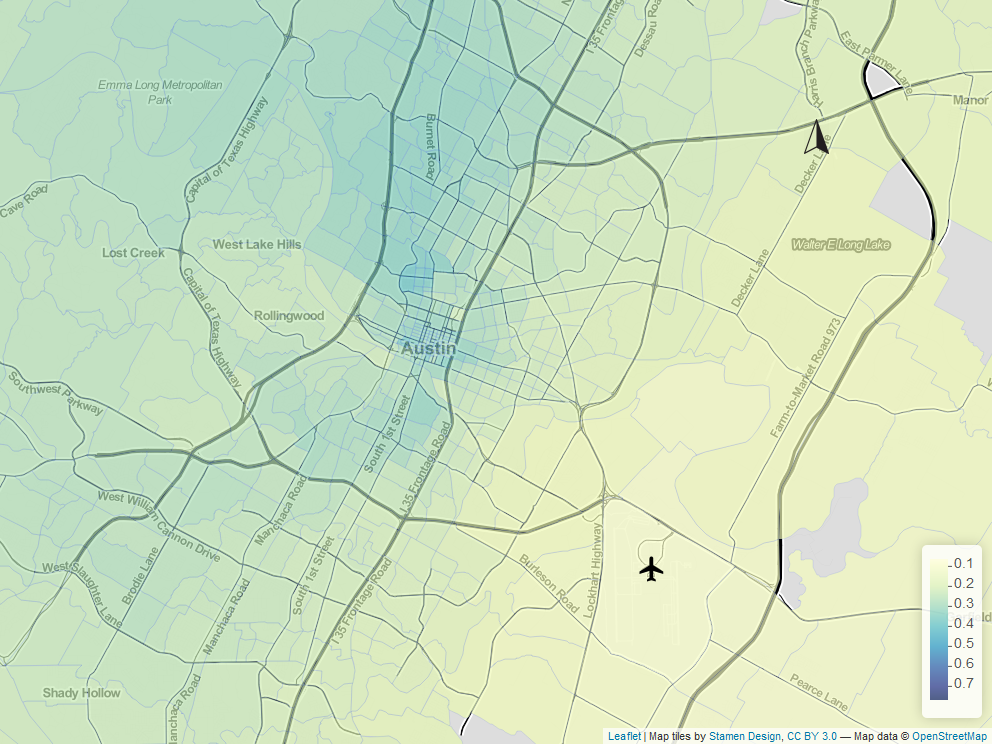
\includegraphics[width=\linewidth]{img/tailprob_34_74__168.png}
        \subcaption{Saturday 11pm (weekend social low traffic)}
        \label{fig:wages:appendix3:d}
    \end{minipage}
    \caption{Probability of exceeding \$34.74 in the next hour given a current location (living wage with costs for one adult with two children).}
    \label{fig:wages:appendix3}
\end{figure}

\section{Quantiles}
\label{appendix:quantiles}


\begin{figure}[htb]
    \centering
    \begin{minipage}[t]{0.48\linewidth}
        \centering
        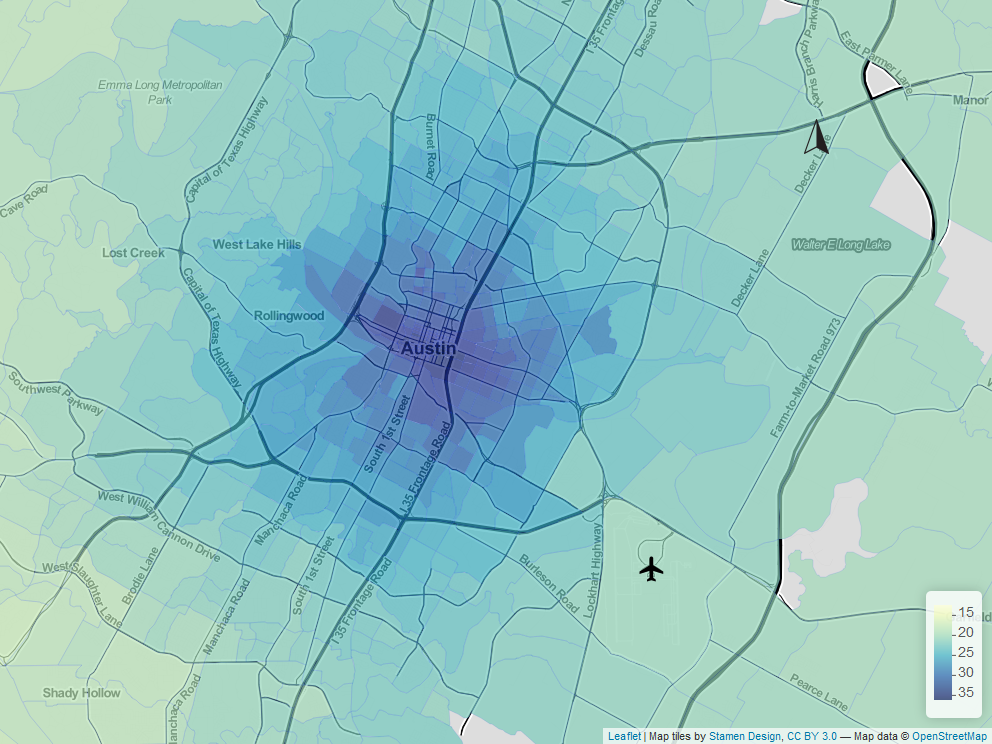
\includegraphics[width=\linewidth]{img/quantile_9_25.png}
        \subcaption{Sunday 8am (weekend low traffic)}
        \label{fig:quantiles:0.25:a}
    \end{minipage}
    \begin{minipage}[t]{0.48\linewidth}
        \centering
        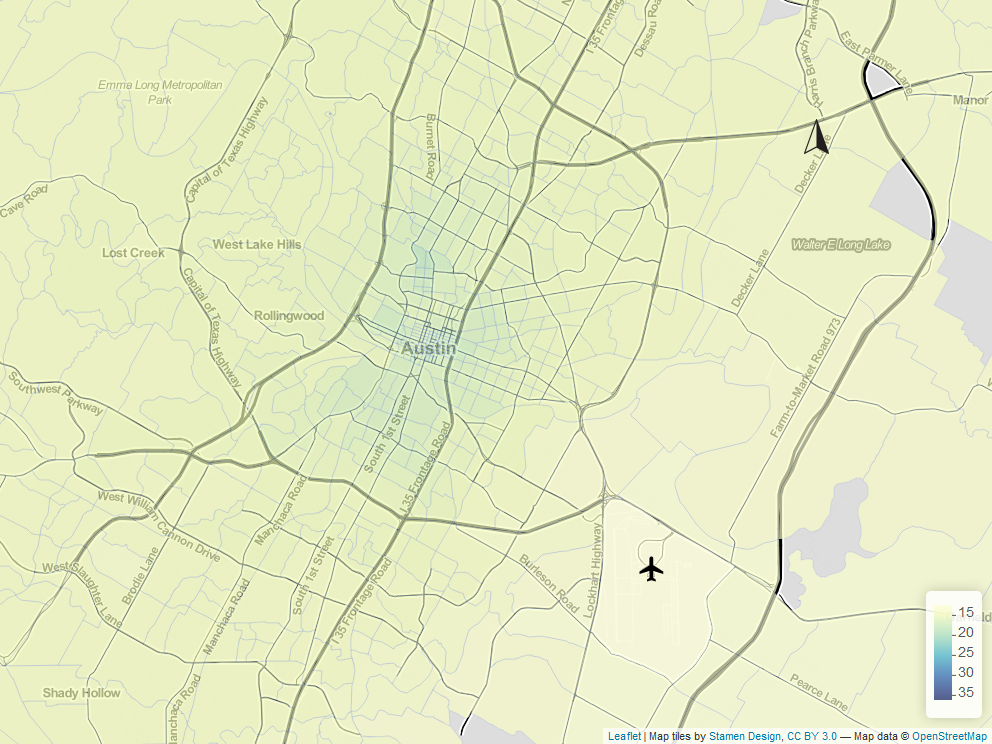
\includegraphics[width=\linewidth]{img/quantile_43_25.png}
        \subcaption{Monday 6pm (weekday rush hour)}
        \label{fig:quantiles:0.25:b}
    \end{minipage}\hfill
    \begin{minipage}[t]{.48\linewidth}
        \centering
        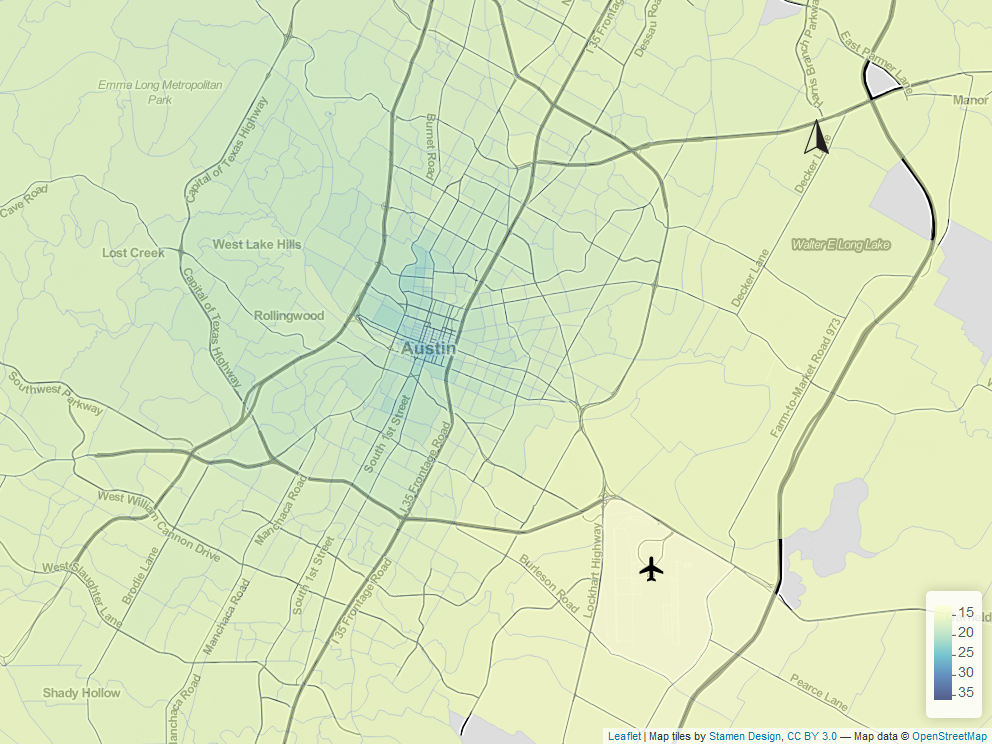
\includegraphics[width=\linewidth]{img/quantile_142_25.png}
        \subcaption{Friday 9pm (weekday social mild traffic)}
        \label{fig:quantiles:0.25:c}
    \end{minipage}
    \begin{minipage}[t]{0.48\linewidth}
        \centering
        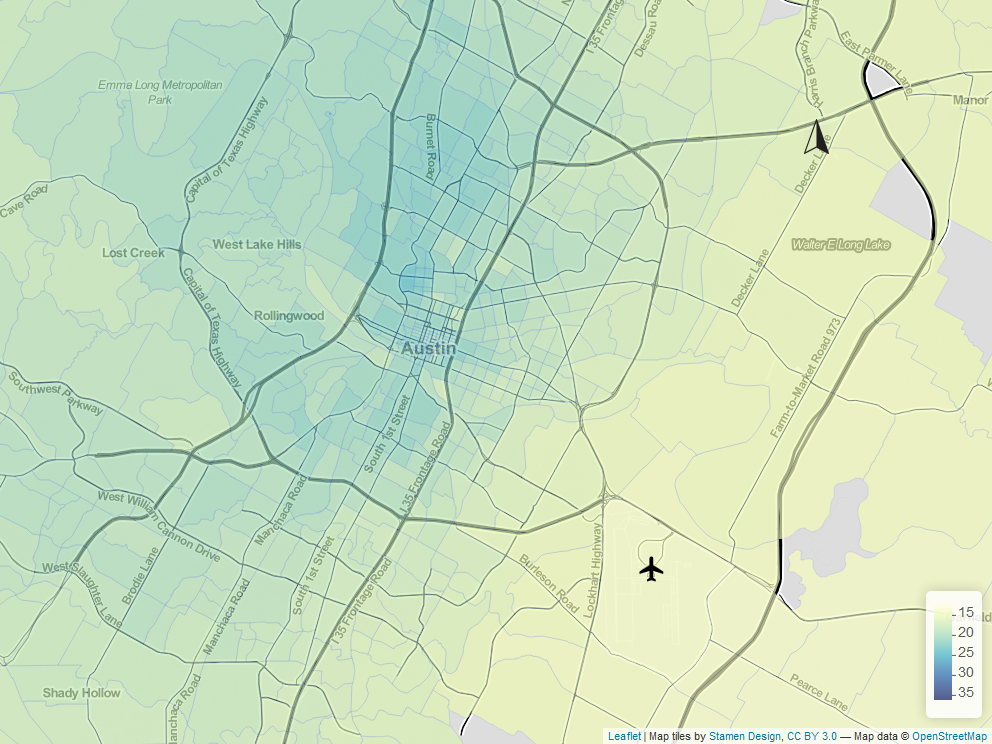
\includegraphics[width=\linewidth]{img/quantile_168_25.png}
        \subcaption{Saturday 11pm (weekend social low traffic)}
        \label{fig:quantiles:0.25:d}
    \end{minipage}
    \caption{Lower 25\% quantile of productivity for different times and locations.}
    \label{fig:quantiles:0.25}
\end{figure}



\begin{figure}[htb]
    \centering
    \begin{minipage}[t]{0.48\linewidth}
        \centering
        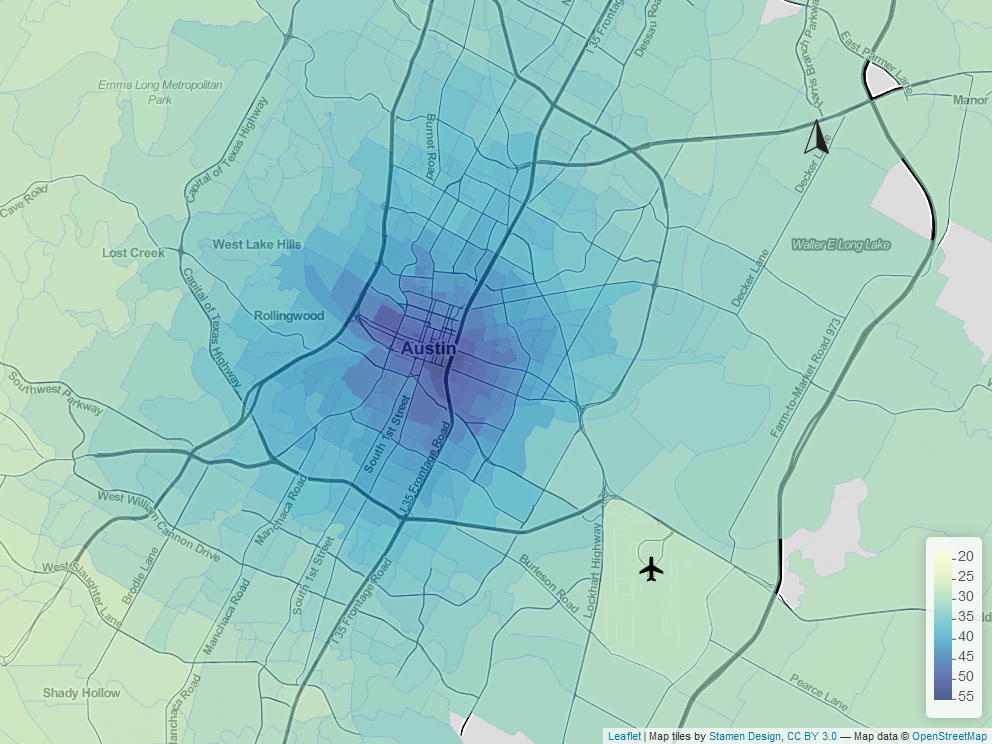
\includegraphics[width=\linewidth]{img/quantile_9_5.png}
        \subcaption{Sunday 8am (weekend low traffic)}
        \label{fig:quantiles:0.5:a}
    \end{minipage}
    \begin{minipage}[t]{0.48\linewidth}
        \centering
        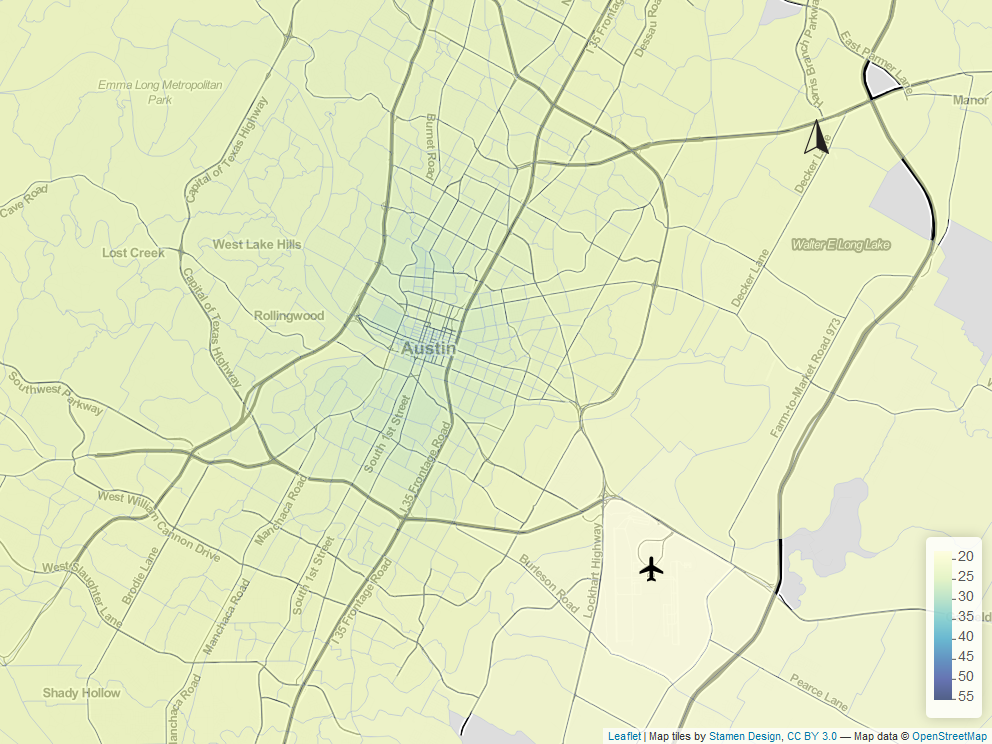
\includegraphics[width=\linewidth]{img/quantile_43_5.png}
        \subcaption{Monday 6pm (weekday rush hour)}
        \label{fig:quantiles:0.5:b}
    \end{minipage}\hfill
    \begin{minipage}[t]{.48\linewidth}
        \centering
        \includegraphics[width=\linewidth]{img/quantile_142_5.png}
        \subcaption{Friday 9pm (weekday social mild traffic)}
        \label{fig:quantiles:0.5:c}
    \end{minipage}
    \begin{minipage}[t]{0.48\linewidth}
        \centering
        \includegraphics[width=\linewidth]{img/quantile_168_5.png}
        \subcaption{Saturday 11pm (weekend social low traffic)}
        \label{fig:quantiles:0.5:d}
    \end{minipage}
    \caption{Median of productivity for different times and locations.}
    \label{fig:quantiles:0.5}
\end{figure}

% \bigskip
% \begin{center}
% {\large\bf SUPPLEMENTARY MATERIAL}
% \end{center}

% \begin{description}

% \item[Title:] Brief description. (file type)

% \end{description}

% \bibliographystyle{Chicago}
\bibliography{ref}

\end{document}
